%%% Hlavní soubor. Zde se definují základní parametry a odkazuje se na ostatní části. %%%

%% Verze pro jednostranný tisk:
% Okraje: levý 40mm, pravý 25mm, horní a dolní 25mm
% (ale pozor, LaTeX si sám přidává 1in)
\documentclass[12pt,a4paper]{report}

%\includeonly{chap2}

\setlength\textwidth{145mm}
\setlength\textheight{247mm}
\setlength\oddsidemargin{15mm}
\setlength\evensidemargin{15mm}
\setlength\topmargin{0mm}
\setlength\headsep{0mm}
\setlength\headheight{0mm}
% \openright zařídí, aby následující text začínal na pravé straně knihy
\let\openright=\clearpage

%% Pokud tiskneme oboustranně:
% \documentclass[12pt,a4paper,twoside,openright]{report}
% \setlength\textwidth{145mm}
% \setlength\textheight{247mm}
% \setlength\oddsidemargin{15mm}
% \setlength\evensidemargin{0mm}
% \setlength\topmargin{0mm}
% \setlength\headsep{0mm}
% \setlength\headheight{0mm}
% \let\openright=\cleardoublepage

%% Použité kódování znaků: obvykle latin2, cp1250 nebo utf8:
\usepackage[utf8]{inputenc}

%% Ostatní balíčky
\usepackage{graphicx}
\usepackage{amsthm}
\usepackage{amsmath}
\usepackage{amsfonts}
\usepackage{todonotes}
\usepackage{longtable}
\usepackage{caption}
\usepackage{float}
\usepackage{xcolor,colortbl}
\usepackage[ruled,linesnumbered,lined,boxed]{algorithm2e}
\usepackage{framed}
\usepackage{multirow}
\usepackage{booktabs}
\usepackage[refpages]{gloss}
\makegloss

\colorlet{shadecolor}{gray!50}

\usepackage{adjustbox}
\usepackage{array}

\newcolumntype{R}[2]{%
	>{\adjustbox{angle=#1,lap=\width-(#2)}\bgroup}%
	l%
	<{\egroup}%
}
\newcommand*\rot{\multicolumn{1}{R{45}{1em}}}% no optional argument here, please!

\makeatletter
\def\BState{\State\hskip-\ALG@thistlm}
\makeatother

\newtheorem{definition}{Definition}
\newtheorem{corollary}{Corollary}
\newtheorem{theorem}{Theorem}
\newtheorem{observation}{Observation}

\newcommand{\attributeDistance}{\delta}
\newcommand{\globalDistance}{\Delta}
\newcommand{\dummy}{dummy}
\newcommand{\dummyoutside}{dummy_n}
\newcommand{\dummyinside}{dummy_a}

%% Balíček hyperref, kterým jdou vyrábět klikací odkazy v PDF,
%% ale hlavně ho používáme k uložení metadat do PDF (včetně obsahu).
%% POZOR, nezapomeňte vyplnit jméno práce a autora.
%\usepackage[ps2pdf,unicode]{hyperref}   % Musí být za všemi ostatními balíčky
%\hypersetup{pdftitle=Název práce}
%\hypersetup{pdfauthor=Jméno Příjmení}

%%% Drobné úpravy stylu

% Tato makra přesvědčují mírně ošklivým trikem LaTeX, aby hlavičky kapitol
% sázel příčetněji a nevynechával nad nimi spoustu místa. Směle ignorujte.
%\makeatletter
%\def\@makechapterhead#1{
%  {\parindent \z@ \raggedright \normalfont
%   \Huge\bfseries \thechapter. #1
%   \par\nobreak
%   \vskip 20\p@
%}}
%\def\@makeschapterhead#1{
%  {\parindent \z@ \raggedright \normalfont
%   \Huge\bfseries #1
%   \par\nobreak
%   \vskip 20\p@
%}}
%\makeatother

% Toto makro definuje kapitolu, která není očíslovaná, ale je uvedena v obsahu.
\def\chapwithtoc#1{
\chapter*{#1}
\addcontentsline{toc}{chapter}{#1}
}


\begin{document}

% Trochu volnější nastavení dělení slov, než je default.
\lefthyphenmin=2
\righthyphenmin=2

%%% Titulní strana práce

\pagestyle{empty}
\begin{center}

\large

Charles University in Prague

\medskip

Faculty of Mathematics and Physics

\vfill

{\bf\Large DOCTORAL THESIS}

\vfill

\centerline{\mbox{
\includegraphics[width=60mm]{Images/mffLogo.png}}}

\vfill
\vspace{5mm}

{\LARGE Jakub Šmíd}

\vspace{15mm}

% Název práce přesně podle zadání
{\LARGE\bfseries Computational Intelligence Methods in Metalearning}

\vfill

% Název katedry nebo ústavu, kde byla práce oficiálně zadána
% (dle Organizační struktury MFF UK)
Department of Theoretical Computer Science and Mathematical Logic

\vfill

\begin{tabular}{rl}

Supervisor of the doctoral thesis: & Mgr. Roman Neruda, CSc.  \\
\noalign{\vspace{2mm}}
Study programme: & Computer Science \\
\noalign{\vspace{2mm}}
Study branch: & Theoretical Computer Science \\
\end{tabular}

\vfill

% Zde doplňte rok
Prague 2016

\end{center}

\newpage

%%% Na tomto místě mohou být napsána případná poděkování (vedoucímu práce,
%%% konzultantovi, tomu, kdo zapůjčil software, literaturu apod.)

\openright

\noindent
Pursuing my doctorate has been a long time effort, and I was lucky that many people supported me along the way. 

Roman Neruda, my supervisor, deserves credit for all his advice, inspiring thoughts, all those late night finishes of our conference papers, and amazing pancakes he would prepare for us during our stays abroad. Because of him, the whole period of my study was an extraordinary adventure and one hell of a ride.

I would also like to thank my present and former Ph.D. colleagues -- Martin Pilát, Ondřej Kazík, Klára Pešková, Tomáš Křen, Josef Moudřík, Martin Šlapák, and Jiří Vytasil.
I have enjoyed all our discussions and lunches at Konírna. I am really proud that I had a chance to be a member of the team.

No conference travels or logistics would be possible without the help of Petra Novotná from our faculty. Many thanks.

I am very grateful to my whole family for their ongoing support during my research, especially to my parents. They made this journey possible.

I would further like to express appreciation to my friends who were always there for me. Mainly, Dan Kobr, Veronika Šmídová, Jaroslav Švelch, Milan Plachý, and Tomáš Potužák.

I also deeply value the help of Roman Kučera from Ataccama with speeding up my experiments by kindly providing some extra computational power.

The biggest "Thank you" belongs to my soulmate Zónička. She has bravely supported me throughout the writing, and awaits me every time I return from a conference. She is my favourite hello and hardest goodbye.

\newpage

%%% Strana s čestným prohlášením k disertační práci

\vglue 0pt plus 1fill

\noindent
I declare that I carried out this doctoral thesis independently, and only with the cited
sources, literature and other professional sources.

\medskip\noindent
I understand that my work relates to the rights and obligations under the Act No.
121/2000 Coll., the Copyright Act, as amended, in particular the fact that the Charles
University in Prague has the right to conclude a license agreement on the use of this
work as a school work pursuant to Section 60 paragraph 1 of the Copyright Act.

\vspace{10mm}

\hbox{\hbox to 0.5\hsize{%
In Prague, Czech Republic, June 13, 2016 
\hss}
\linebreak
\hbox to 0.5\hsize{%
\hss}}
\hbox{\hbox to 0.6\hsize{%

		\hss}
	\linebreak
	\hbox to 0.4\hsize{%
		\rule{5cm}{0.5pt}
		\hss}}
\hbox{\hbox to 0.7\hsize{%
		
		\hss}
	\linebreak
	\hbox to 0.3\hsize{%
		Jakub Šmíd
		\hss}}

\vspace{20mm}
\newpage

%%% Povinná informační strana disertační práce

\vbox to 0.5\vsize{
\setlength\parindent{0mm}
\setlength\parskip{5mm}

Název práce:
Metody výpočetní inteligence pro metaučení
% přesně dle zadání

Autor:
Jakub Šmíd

Katedra:  % Případně Ústav:
Katedra teoretické informatiky a matematické logiky
% dle Organizační struktury MFF UK

Vedoucí disertační práce:
Mgr. Roman Neruda, CSc., Ústav informatiky AV ČR, v.v.i.
% dle Organizační struktury MFF UK, případně plný název pracoviště mimo MFF UK

Abstrakt:
% abstrakt v rozsahu 80-200 slov; nejedná se však o opis zadání disertační práce
Tato práce je zaměřena na problematiku výběru algoritmu, která má za cíl doporučit algoritmus strojového učení k nové úloze. Řešení problému vychází z~myšlenky, že se algoritmy chovají podobně na podobných datech. Tato podobnost je často založena na extrakci pevného počtu metaatributů z každé úlohy. Vzhledem k tomu, že počet atributů se u různých úloh typicky liší, ztrácíme tak důležité informace. V této práci popíšeme třídu algoritmů, která dokáže zpracovat také informace o jednotlivých atributech. Naše metody jsou založeny na přiřazování atributů. Výsledná vzdálenost mezi úlohami je dána jako součet vzdáleností mezi atributy určenými optimálním přiřazením. Dále dokážeme, že za určitých podmínek můžeme zaručit, že výsledná vzdálenost mezi úlohami je metrika. Provedeme sadu experimentů na datech extrahovaných z OpenML repozitáře. Vytvoříme vzdálenost mezi atributy prostřednictvím genetických algoritmů, genetického programování a několika regularizačních technik, jako je koevoluce a zavedení vícekriteriality. Výsledky experimentů naznačují, že výsledná vzdálenost mezi úlohami může být úspěšně použita na problematiku výběru algoritmu. Ačkoliv jsme naše metody použili výhradně k metaučení, lze je aplikovat i v jiných oblastech. Navržené algoritmy jsou aplikovatelné kdekoliv, kde máme definovanou vzdálenost mezi prvky nějaké množiny a potřebujeme navrhnout vzdálenost mezi prvky potenční množiny původní množiny.

Klíčová slova:
Metaučení, Strojové učení, Metriky, Genetické algoritmy, \\ Přiřazování atributů

\vss}

\pagebreak
\newpage

\nobreak\vbox to 0.49\vsize{
\setlength\parindent{0mm}
\setlength\parskip{5mm}




Title:
% přesný překlad názvu práce v angličtině
Computational Intelligence Methods in Metalearning

Author:
Jakub Šmíd

Department:
Department of Theoretical Computer Science and Mathematical Logic
% dle Organizační struktury MFF UK v angličtině

Supervisor:
Mgr. Roman Neruda, CSc., Institute of Computer Science, AS CR
% dle Organizační struktury MFF UK, případně plný název pracoviště
% mimo MFF UK v angličtině

Abstract:
% abstrakt v rozsahu 80-200 slov v angličtině; nejedná se však o překlad
% zadání disertační práce
This thesis focuses on the algorithm selection problem, in which the goal is to recommend machine learning algorithms to a new dataset. The idea behind solving this issue is that algorithm performs similarly on similar datasets. The usual approach is to base the similarity measure on the fixed vector of metafeatures extracted out of each dataset. However, as the number of attributes among datasets varies, we may be loosing important information. Herein, we propose a family of algorithms able to handle even the non-propositional representations of datasets. Our methods use the idea of attribute assignment that builds the distance measure between datasets as a sum of distance given by the optimal assignment and an attribute distance measure. Furthermore, we prove that under certain conditions, we can guarantee the resulting dataset distance to be a metric. We carry out a series of metalearning experiments on the data extracted from the OpenML repository. We build up attribute distance using Genetic Algorithms, Genetic Programming and several regularization techniques such as multi-objectivization, coevolution, and bootstrapping. The experiment indicates that the resulting dataset distance can be successfully applied on the algorithm selection problem.
Although we use the proposed distance measures exclusively on metalearning, it is possible to use our methods even beyond this task. The algorithms can handle every situation where we have a notion of distance between elements of some set and are looking to define a distance on the power set of the original set.

Keywords:
% 3 až 5 klíčových slov v angličtině
Metalearning, Machine Learning, Metric, Genetic Algorithms, Attribute Assignment

\vss}

\newpage

%%% Strana s automaticky generovaným obsahem disertační práce. U matematických
%%% prací je přípustné, aby seznam tabulek a zkratek, existují-li, byl umístěn
%%% na začátku práce, místo na jejím konci.

\openright
\pagestyle{plain}
\setcounter{page}{1}
\tableofcontents

%%% Jednotlivé kapitoly práce jsou pro přehlednost uloženy v samostatných souborech
%\chapter*{Introduction}
\addcontentsline{toc}{chapter}{Introduction}


%Introduction
\chapter{Introduction}
The ongoing rapid growth of the available amount of data drives the urge for automated processing of such data.
\emph{Data mining} -- the means of finding new patterns in \emph{datasets} -- is now widely used in medicine, economics, bioinformatics and other important areas of human interest. Many different algorithms exist and are used for this task of pattern extraction. However, even for an expert, it is hard to choose the most suitable algorithm for a particular dataset. 
According to the \emph{No Free Lunch} theorem (NFL) stated in \cite{NoFreeLunchTheorem}, the average performances of data mining algorithms on all data mining problems are equal. It means that elevated performance of any algorithm over one class of problems is paid for in performance over another class. However, NFL considers all possible problems. We are mostly interested in so called \emph{real world} problems. Therefore, the key to success when dealing with a data mining real world problem is in binding the problem with an algorithm having elevated performance on the class of the problem. Since many fields depend on data mining techniques, it is crucial to propose and improve such bindings.

\emph{Metalearning} \cite{BrazdilMetalearning-2009} -- the learning how to learn -- can tackle the issue. 
The main idea behind metalearning is that \emph{machine learning} methods are supposed to perform similarly on similar datasets. Therefore, the notion of dataset similarity is crucial. In most cases, the similarity is computed using data characterizing the datasets -- the \emph{metadata}. Metalearning techniques use the metadata and previous experience to predict the performance of machine learning methods on new datasets. In essence, metalearning does not differ much from the traditional machine learning. The main difference is that metalearning works with the metadata of given datasets instead of the actual data, and that the result of metalearning is a recommendation of a machine learning method to use. 

The metadata may contain general information about the dataset, like the number of instances and attributes, the number of classes, performance of some algorithm over the dataset, etc. There is, however, a fixed amount of such general information extracted out of each dataset.  Many traditional methods compare datasets based on such measures.

The attribute-specific metadata include more fine-grained information about the dataset. On the other hand, each dataset can have a different number of attributes (and consequently, different amount of attribute-specific metadata), which leads to a non-propositional representation of the datasets using attribute-specific metadata. The problem of defining the similarity on the non-propositional space is non-trivial as stated by Kalousis in \cite{RepresentationalIssuesInMetalearning}. The authors of \cite{BrazdilMetalearning-2009} also explicitly recognize the problem of handling datasets described by the varying amount of metafeatures.
In the past there were only few attempts to define the non-propositional similarity. Furthermore, most of these attempts loose important information in the process.

One of the goal of this thesis is to propose algorithms capable of handling such a non-propositional representation. We take into consideration other methods dealing with non-propositional data, either directly in the metalearning field or in other fields as well.
Another goal of this thesis is to investigate theoretical properties of proposed distance measures and compare them with the related state of the art methods. We investigate whether the methods satisfy \emph{metric} axioms, alternatively, what properties must be satisfied in order to do so.

The performance of the proposed methods should be evaluated on data. Several machine learning repositories are reviewed. The emphasis is put on the amount of data provided, types of metadata available, and the fact whether the data are publicly accessible allowing for the independent re-evaluation of our results.


\section{Outline of the Thesis}
The structure of the thesis is as follows. Chapter \ref{chapter:preliminaries} introduces the field of metalearning. Different types of scenarios addressed by metalearning are presented. The literature that covers different ideas and advances in metalearning is reviewed. The algorithm ranking based on distance measures is addressed in more depth. Unified workflow for measuring the quality of distance based algorithm ranking is presented. We also cover some of our contributions related to metalearning that are not directly related to the main goals of the thesis. This includes our recommendation multi-agent system \emph{Pikater} and a \emph{hierarchical clustering} approach for metalearning.  

Chapter \ref{chapter:globalDistance} reviews the metric spaces and several well known facts about metrics spaces. We look into the commonly used dataset distance measures based on the fixed amount of metadata extracted from datasets and what properties are necessary in order to get a metric.

The main contribution of the thesis is presented in Chapter \ref{chapter:attributeAssignment}. First, we discuss the motivation behind dealing with objects with variable structure and review some work not directly related to metalearning, which however served as an inspiration for the work in this thesis. We also discuss why we cannot use such techniques to address the variable amount of attributes when comparing the datasets. We review state of the art approaches to handle the attribute-specific metadata in metalearning and discuss their strengths and weaknesses. The idea of attribute assignment is presented. The main idea lies in defining attribute distance measure and aligning the attributes as best as we can. The desired distance between datasets is the sum of distances between aligned attributes. Several algorithms based on this idea are proposed. We also show what properties we have to maintain in order to get the metric on the dataset space. We also discuss other ideas we considered, which could, however, violate some of metric axioms.

Chapter \ref{chapter:obtainingData} discusses data needed to conduct our experiments. Several databases of machine learning datasets are reviewed including those containing results of machine learning algorithms over those datasets. We discuss the metadata available about the datasets and establish attribute-specific metadata that we will extract ourselves in order to be able to build attribute assignment models.

The first batch of experiments is proposed in Chapter \ref{chapter:metricExperiments}. All the pieces and algorithms are glued together and the workflow is reviewed as a whole. Experiments are proposed in such a way that we always get a metric on the dataset level. We let the \emph{Genetic Algorithms} \cite{HollandGeneticAlgorithms} optimize weights of the attribute assignment techniques. We also review the complexity of the whole workflow that will be important when proposing the experiment settings. Our experiments will be actually solving \emph{reinforcement learning} \cite{aima3ed} task with very rare feedback from the environment. The results of experiments are discussed and compared between themselves and a \emph{baseline} algorithm. 

Chapter \ref{chapter:metricRelaxation} introduces more expressive language to describe attribute distance measure while relaxing the requirement on dataset metric. We will show that the relaxation will guarantee a semimetric on the attribute space. We discuss whether the missing triangle inequality is necessarily important for the distance measure. We will also prove that the semimetric on the attribute level lead to a semimetric on the dataset level using our attribute assignment workflow. We conduct another batch of experiments with the new algorithms, and discuss their results.

In Chapter \ref{chapter:regularization}, we discuss set of techniques that could improve the generalization abilities of some of our models. In particular, we discuss coevolution, bloat control and bootstrapping  of the population as an extension of the genetic algorithms. We also discuss using \emph{multi-objectivization} to split the objective function into two. The second -- added -- criterion is the metric similarity. We also define the \emph{multi-objective optimization} and describe one algorithm in particular -- \emph{NSGA-II} \cite{nsgaII}. We conduct experiments with coevolution, bootstrapping and bloat control and compare their results with the previous experiments. We review one of our previous works  with multi-objectivization.

Chapter \ref{chapter:conclusion} concludes the thesis. The goals of the thesis are evaluated based on the expectations. The future work and possible opportunities to improve the results are outlined.

 

 
%Related work - also ours
\chapter{Preliminaries}
\label{chapter:preliminaries}
This chapter introduces metalearning -- learning how to learn. We begin with defining instances of data called datasets using a relation theory. We also discuss possible domains of relations and establish some restrictions for the rest of the thesis. The space of datasets is defined. We elaborate on specific problems that are connected with defining a structure on this space. Machine learning tasks are introduced and divided into three basic types -- \emph{supervised}, \emph{unsupervised} and \emph{reinforcement learning} -- based on the amount of feedback received from the environment. Then, we discuss the means to evaluate the performance of machine learning algorithms over machine learning tasks, namely \emph{root mean squared error}, \emph{F-measure} and \emph{predictive accuracy}. We discuss the existence of algorithm outperforming all other algorithms. We elaborate on the No Free Lunch theorem \cite{NoFreeLunchTheorem} and its implication on the machine learning tasks. The work of Smith-Miles et al. is reviewed \cite{SmithMilesTowardsMeasuresOfAlgorithmPerformance} as an interesting example of finding algorithms dominating a subset of data. We define the task of metalearning and we provide several examples of it -- dynamic parameter adjustment, and recommending machine learning algorithms for a given -- not yet seen -- task. The different algorithm recommendation are analysed, depending on the amount of information one requires from recommendation techniques - single algorithm, subset of them, more detailed ranking or even estimating the performance of algorithms. We discuss how generic methods for algorithm ranking should look like and define distance based ranking. We also review some of the related literature including our own results with hierarchical clustering \cite{jaICMLA2013}. Means of measuring the quality of a ranking are provided. The very simple and often effective baseline algorithm for the ranking task is introduced. The different types of performance indicators are reviewed together with some interesting approaches how to combine accuracy and time. Different types of metadata are defined. State of the art means of utilizing such metadata for the sake of algorithm recommendation are reviewed. We introduce a concept of automated systems able to handle the whole task of metalearning. Our own recommendation system Pikater is reviewed. We discuss PCA \cite{pca} method that can be used for visualization of multi-dimensional data.

\section{Datasets}
\label{section:datasets}
Dataset describes the instance of data. It can be a relation, set of graphs, collection of texts or database of proteins. Throughout this thesis, unless mentioned otherwise, we will consider the dataset to be of a form of relation \cite{dbRelation}.

\begin{definition}
	\emph{Relation} is a set of tuples $(d_1, \dots, d_n)$, where each element $d_j$ is a member of $D_j$, a data domain or data type.
\end{definition}

Given the relation, the dataset itself has a structure in the sense that every row is a vector of the same size and from the domain given by $D_1, \dots , D_n$. Alternatively, one can look at a dataset as a list of columns where every column has a domain and a collection of values. Sizes of all collections are the same.

We will specify three basic allowed supertypes:
\begin{enumerate}
	\item \emph{Categorical} supertype - domain is a finite set of values sometimes referred to as labels.
	\item \emph{Numerical} supertype - domains are real numbers -- $\mathbb{R}$.
	\item \emph{Integer} supertype - domains are integer numbers -- $\mathbb{N}$.
\end{enumerate}
Based on these supertypes, we will put domain restrictions on datasets that will be considered in this thesis. Every domain must be one of the defined supertype, possibly equal to the supertype or with some other restrictions (e.g. specified minimum, maximum). In this sense, the numerical supertype is also a supertype of the integer supertype. We have decided to distinguish this special case, as additional useful properties may be defined for the integer supertype only. We will also allow for some values to be undefined (missing).

We will define \emph{dataset space} as the space of all possible datasets. It is important to consider that now the dataset space is merely a set
without any added structure. Although every dataset has a structure defined by the relation, one cannot easily follow this when proposing a structure on the dataset space for the following reasons:
\begin{itemize}
	\item Number of columns may differ: the arity of relations representing datasets may vary. 
	\item Domains may differ: domains of columns may be different.
	\item Number of rows may differ: the cardinality of relations may differ.
\end{itemize}
Adding the structure into the dataset space is one of the main topics in the rest of the thesis.
\section{Machine Learning Tasks}
\label{section:mlTasks}
\emph{Machine learning} is a subfield of computer science. We say that algorithm is learning if it improves its performance on future tasks after making observations (receiving feedback) about the world \cite{aima3ed}.
According to the type of feedback, we can distinguish three main types of machine learning tasks.
\begin{definition}
	In \emph{unsupervised learning}, no explicit feedback is provided.
\end{definition}
A common unsupervised learning task is \emph{clustering}, when we try to sort input data to potentially interesting clusters. For example, an algorithm can eventually develop a concept of sunny and rainy days without ever being told this distinction.

On the opposite side stands the task of supervised learning, when we provide a teacher knowing the correct answers. Given a dataset, set of columns (usually only one) is designated as a target. 
\begin{definition}
	The task of \emph{supervised learning} is this: \\
	Given a \emph{training set} of $n$ example input-output pairs (rows of dataset)
	\begin{equation*}
	(x_1,y_1),\dots (x_n,y_n),
	\end{equation*}
	where $y_i$ is a vector of values of target columns of row $i$, $x_i$ is a vector of values of the remaining columns, each $y_i$ was generated by an unknown function $y=f(x)$, 
	discover a function $h$ that approximates the \emph{true function} f.
\end{definition}
 The function $h$ is called \emph{hypothesis}. The goal of learning is to search space of possible hypotheses finding the one that performs well, even on new examples beyond the training set. Note that in more general case, the input-output pair $x$ and $y$ do not have to be numbers or vectors, they can be labels, graphs or even more complex objects.

If the target attribute is only a single column, basic types of supervised learning can be defined by distinguishing the tasks according to the domain of target column $y$ -- classification or regression. 
In classification, we are assigning some labels to the input $x$. For example, when forecasting tomorrow's weather based on today's lookout, we could assign either sunny, cloudy or rainy.
\begin{definition}
	\emph{Classification} is a supervised learning task where the output y is one of the finite set of values. If the cardinality of the set is 2, we say it is a \emph{binary} or \emph{boolean} classification.
\end{definition}
On the other hand, in regression we are estimating some numeric value like tomorrow's temperature given today outlook.
\begin{definition}
	\emph{Regression} is a supervised learning task where the output y is a real number.
\end{definition}

To measure the quality of some hypothesis, the \emph{testing set} of previously unseen examples is given to the hypothesis. We say that $h$ \emph{generalizes} well if it correctly predicts the value $y$ for novel examples in the testing set. Sometimes, the learning algorithm exhibits low error on the training set while having poor generalization abilities. This phenomenon is called as \emph{overfitting} as the algorithm learned properties that are only specific for the training set. Usually, the algorithm capable of creating complex models tend to overfit on the simple data. To tackle this, the concept of \emph{ Occam's razor} is often used. If we have two hypothesis having similar performance, we should prefer the model with the lower complexity \cite{aima3ed}.

There are many ways of how to measure the quality of the hypothesis. We will list a few:

\begin{definition}
	\emph{Root mean squared error} (RMSE) of some hypothesis $h$ is defined as 
	\begin{equation*}
	RMSE(h)=\sqrt{\sum_{i=1}^{n}\frac{(h(x_i)-f(x_i))^2}{n}},
	\end{equation*}
	where $n$ is the number of samples in the testing set.
\end{definition}


In the binary classification we can define precision and recall:
\begin{definition}
	\emph{Precision} and \emph{recall} are defined as
	\begin{equation*}
	precision = \frac{tp}{tp+fp},
	\end{equation*}
	\begin{equation*}
	recall = \frac{tp}{tp+fn},
	\end{equation*}
	where $tp$ stands for true positive -- number of cases the classifier answered 1 correctly. Analogically, we can define $fp$ and $fn$ -- false positives and false negatives. They denote number of cases when classifier incorrectly answered 1 or 0 respectively.
\end{definition}
The common way to measure the quality of binary classifier is F-measure -- the harmonic mean of precision and recall.
\begin{definition}
	\emph{F-measure} of the hypothesis is
	\begin{equation*}
	F(h)=2\frac{precision\times recall}{precision+recall}.
	\end{equation*}
\end{definition}

In classification tasks, we can define the percentage of classes that were classified correctly or incorrectly resulting into the Predictive Accuracy and Error Rate. 

\begin{definition}
	\label{definition:predictiveAccuracy}
	\emph{Predictive Accuracy} is defined as
	\begin{equation*}
	PredictiveAccuracy = \frac{\#(h(x_i)=f(x_i))}{n},
	\end{equation*}
	where $n$ is the number of samples in the testing set.
	\emph{Error Rate} is defined as 
	\begin{equation*}
	ErrorRate = 1 - PredictiveAccuracy = \frac{\#(h(x_i)\ne f(x_i))}{n},
	\end{equation*}
	where $h$ is the hypothesis, $f$ is the true function, $n$ is the number of samples and $\#$ denotes the number of cases for which the argument is True.
\end{definition}

In the real world scenario, the reward is not often associated with every action. We often get a reward (or punishment) after a series of decisions. For example, if somebody wants to get from one place A to another place B, with every step taken he does not know whether the step was right. He can evaluate his decisions after he successfully gets to place B for example based on the time, money and energy needed to get to the destination. This concept is formalized as a third learning scenario -- reinforcement learning:
\begin{definition}
	The basic \emph{reinforcement learning} model consists of:
	\begin{enumerate}
		\item A set of environment states S.
		\item A set of actions A.
		\item Rules of transitioning between states.
		\item Rules that determine the scalar immediate reward of a transition.
		\item Rules that describe what the agent observes.
	\end{enumerate}
\end{definition}

\section{Metalearning}
This section describes the task of metalearning. Intuitively, it is a task of learning how to learn. We will discuss the metalearning task in general and then move to one particular subset of metalearning tasks -- algorithm recommendation. We will create a taxonomy of recommendation based on properties we would like to recommend.

\subsection{Metalearning Task}
In the recent years, many algorithms were proposed to solve different machine learning tasks. Usually, every such algorithm has many parameters and its performance is heavily dependent on settings of those parameters. Even for an expert, it is sometimes difficult to choose the right algorithm and set up the parameters correctly. Furthermore, scientists from different fields than computer science face great challenges when trying to employ machine learning to solve their tasks. It would be useful if such a system was provided that would either solve the machine learning tasks directly or would assist in choosing the right algorithms and parameters. Such a tool should learn from a previous experience. The common idea behind such recommendation tool is based on the idea that algorithms perform similarly on similar datasets.

One could also improve based on the past experience in adjusting the parameters. For example, if one non-deterministic machine learning experiment did not achieve desired performance for hundreds of attempts with the same parameter settings, it could be perhaps a good idea to try different settings next time. Also, if some indicators would suggest that the algorithm was being stuck in some local optimum, the parameters of the algorithm could be adjusted ad hoc, so the local optima are avoided and algorithm hopefully converges to a global optimum. The authors of \cite{algorithmControl} review the dynamic control of parameters for many nature inspired algorithms.

In transfer learning, we try to transfer some learned properties to a new -- similar -- task. For example, authors of \cite{TransferabilityDeepNeuralNetworks} argue that deep neural networks often learn a generally useful concept in the top layers and that such knowledge can be transferred to other tasks. The ability to transfer knowledge depends on the similarity of tasks.

These scenarios have some common patterns. In each case above, we are utilizing some extra knowledge -- previous experience or notion of dataset similarity -- usually referred to as \emph{metaknowledge}. This continuous process of learning how to learn is often denoted as metalearning.
In \cite{BrazdilMetalearning-2009}, we can find more formal definition of metalearning:
\begin{definition}
	\emph{Metalearning} is the study of principled methods that exploit metaknowledge to obtain efficient models and solutions by adapting machine learning and data mining processes.
\end{definition}

In this thesis, we will focus on the first case -- the \emph{algorithm selection} -- in which we use metaknowledge to recommend the best algorithms, parameters or both to some machine learning task. The problem was originally stated in 1976 by Rice \cite{1976RiceAlgorithmSelectionProblem} and received much attention from the research community ever since. Rice devised a general framework to select the best algorithm for a problem at hand. He suggested to extract set of \emph{metafeatures} out of a given problem and use these metafeatures to select an algorithm that maximizes the expected performance of the algorithm on the problem at hand.

One could naturally ask whether such recommendation is needed in the first place. Perhaps there exists an algorithm that is outperforming every other algorithm on every task. The answer is no. According to the \emph{No Free Lunch} theorem stated in \cite{NoFreeLunchTheorem}, the average performances of data mining algorithms on all data mining problems are equal. It can still be the case that there are some areas that are dominated by certain algorithms.

For instance, in \cite{SmithMilesTowardsMeasuresOfAlgorithmPerformance}, Smith-Miles et al. investigated different instances of optimization problems and features describing differences between these instances. The PCA (see Section \ref{section:pca}) was used to map features into two dimensional space.
Another instances were generated so the projected two dimensional space was better covered. The search algorithms were employed to find instances that are hard for each solver and provided a map of search space based on the expected footsteps of different optimization algorithms. The projected space of instances were coloured
according to colour of the dominating optimization technique on that space. This gave a nice overview of which part of two dimensional space computed by the PCA algorithm was dominated by which optimisation algorithm. This can be seen in Figure \ref{fig:smithMilesDominatedSpace}.

\begin{figure}
	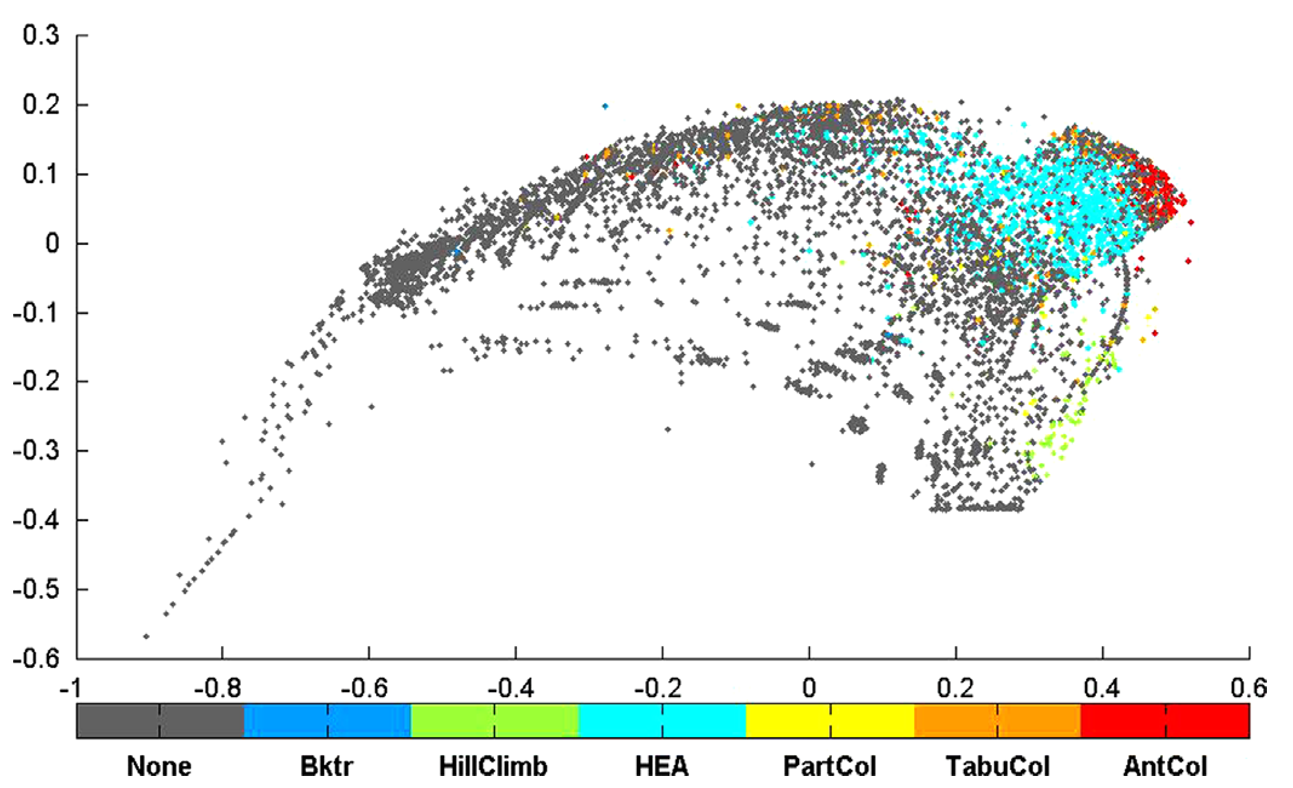
\includegraphics[width=14cm]{Images/smithMilesDominatedSpace.png}
	\centering
	\caption{Space of optimisation problems was projected to two dimensions by the PCA algorithm and coloured according to the best algorithm in that area. Grey colour is for the instances that had multiple best algorithms (according to some small margin) \cite{SmithMilesTowardsMeasuresOfAlgorithmPerformance}.}
	\label{fig:smithMilesDominatedSpace}	
\end{figure}


Another way to look at the No Free Lunch theorem is the fact that lots of problems from the set of all data mining problems may not be particularly interesting. One could argue that only problems related to some useful problem are worth considering. This argument is supported by the observation that usually when one learns something, he expects that the function being learned has some nice properties. For instance, it is continuous and close points have the same or similar value. For example, a car does not stop being a car if it changes a colour. One would have to make multiple adjustments to destroy the car properties. This arguing gives the notion to vaguely defined \emph{real world} problems. It follows that one should not be too concerned about the No Free Lunch theorem as it may still be the case that there is an algorithm outperforming every other algorithms on the real world problems.

In the rest of the thesis, we will solely focus on the algorithm selection problem.

\subsection{Types of Recommendation}
We can distinguish different types of algorithm selection \cite{BrazdilMetalearning-2009} based on what exactly we want to predict -- the \emph{metatarget}:
\begin{enumerate}
	\item Best in set.
	\item Best subset.
	\item Ranking.
	\item Performance prediction.
\end{enumerate}

The simplest case is choosing the best algorithm among the set of algorithms. This case has the advantage that it can be formulated as a classification problem. The major disadvantage is that if this algorithm produces unsatisfactory result, the recommendation system does not clue any steps to take further on. One may also choose to predict the best parameter for a certain algorithm.

More complicated case is when one is interested in some smaller subset of algorithms or parameters. The algorithms selected are those performing well -- this is often described as performing well within a margin. In the case of classification, the margin can be defined as 
\begin{equation}
\left[ e_{min}, e_{min}+k\sqrt{\frac{e_{min}(1-e_{min})}{n}} \right),
\end{equation}
where $e_{min}$ is the error of the best algorithm, $n$ is the number of examples and $k$ is a user-defined parameter determining the size of the margin.

Other alternative it to carry out statistical testing. The selected algorithms  will be those with not significantly worse performance than the best. Best subset address some flaws of the first type, however user does not have any guidance with the order of algorithms to try. Similarly, there is no guidance if all algorithms from the subset were tried.

In ranking, the goal is to rank (sort) algorithms or parameters according to their expected performance. In this case the exact performance value is not important, one is simply interested in the rank itself. One would naturally expect complete total ordering between algorithms or parameters. This does not have to be the case, sometimes this level of granularity is not desirable. For instance, one can decide that the algorithms with the similar expected performance will be inserted to a certain class and define the ordering just between the different classes of algorithms. The ordering between the algorithms of the same class could remain undefined. 

Based on these, we can distinguish different types of ranking based on the level of granularity provided. We can recognize linear and weak rankings (whether ranking defines linear order on some set of algorithms) and complete and incomplete rankings (whether rankings include all algorithms or just a subset). Rankings can be represented by \emph{Hasse diagrams} -- examples are in Figure \ref{fig:rankingTypes}.

\begin{figure}
	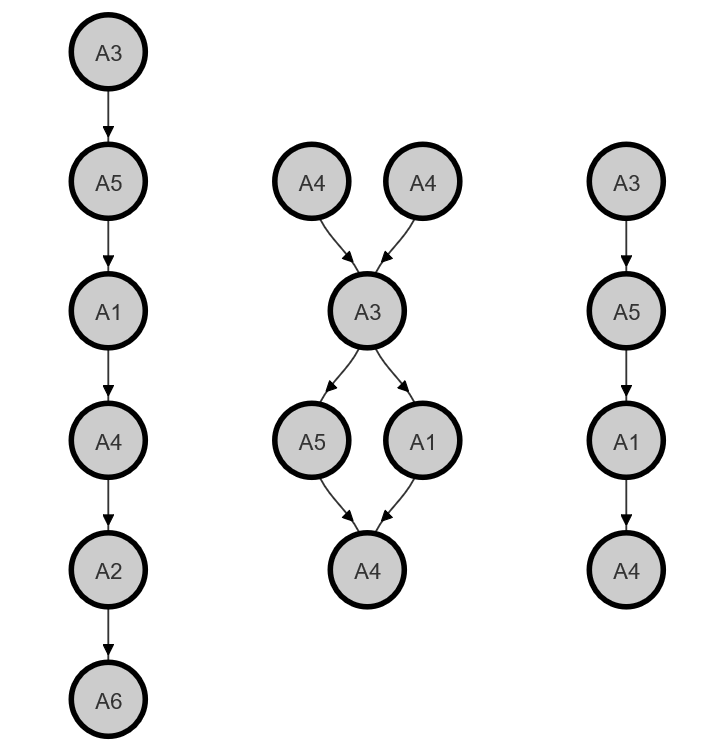
\includegraphics[width=8cm]{Images/rankingTypes.png}
	\centering
	\caption{Types of ranking. The left one is linear complete, middle one is weak and complete and the ranking on the right is linear and incomplete. Adapted from \cite{BrazdilMetalearning-2009}.}
	\label{fig:rankingTypes}	
\end{figure}

In some cases, one is not only interested in the ranking, but also in the performance estimation. This can be useful if there are some requirements for the minimal performance acceptable or if more detailed information about the expected outcome are required. It also makes sense if the estimated performance is the runtime of algorithm, as resources could be either limited or expensive, and algorithms that are expected to finish quickly are preferred. One could also expect that faster algorithms produce simpler hypothesis, thus arguing that on simple problems faster algorithms will have better generalization abilities by Occam's razor. 
The performance estimations can be easily transformed to ranking by ordering the algorithms by their estimated performance. 

Authors of \cite{evolutionaryProgramPredictingPerformance} propose a practical model of \emph{Evolutionary Program-induction Algorithms} (EPAs) including Genetic Programming (Section \ref{section:geneticProgramming}). The model corresponds to the following equation:
\begin{equation}
P(t) \approx a_0 + \sum_{p \in S}a_pd(p,t),
\end{equation}
where $a_i$ are coefficients, $P(t)$ is a performance of an EPA on the target functionality $t$, $S$ is a subset of a program search space and $d$ is a function of similarity between the output of the EPA and the target functionality $t$. The paper deals with the issue of determining the suitable coefficients and the suitable subset of the search space. The model is tested on various tasks.

In \cite{diplomka, jaIcannga2013}, we have predicted accuracy and expected time consumption  for some algorithm on a new dataset using the data gathered by our recommender system Pikater (see Section \ref{section:recommenderSystems}). A unique non-propositional distance measure was used (see Algorithm \ref{algo:attributeAlignmentMasterThesis}). 
Estimation functions were evolved by Genetic Programming and were represented by two trees: one for estimating accuracy and another one for estimating time consumption. The GP algorithm included terminals representing distance and the performance result (either accuracy or duration depending on the tree being evolved) from one of the nearest dataset. Randomly initialized constant terminal specified which nearest dataset was used. The special terminal estimating complexity was proposed: 
\begin{equation}
complexity = \sum_{a_i}\sigma(a_i)\log(n_{rows}),
\end{equation}
where $n_{rows}$ measures number of rows in the datasets, $a_i$ is the $i$-th attribute and $\sigma(a_i)$ estimates the attribute complexity based on its type:
	\begin{equation}
	\sigma(a_i)=
	\begin{cases}
	1; \text{ if  } a_i \text{ is a boolean or categorical attribute}, \\
	2; \text{ if  } a_i \text{ is an integer attribute}, \\
	3; \text{ if  } a_i \text{ is a real attribute}.
	\end{cases}
	\end{equation}
We argued that continuous and numerical attributes are usually hard to process, hence the increased coefficient. This complexity terminal proved especially useful for estimating the time needed to conduct the experiment.
The example of an evolved recommendation tree is in Figure \ref{fig:masterThesisTree}.
The recommendation agent utilizing the evolved estimation trees was implemented into our custom metalearning system called Pikater (see Section \ref{section:recommenderSystems}).

\begin{figure}
	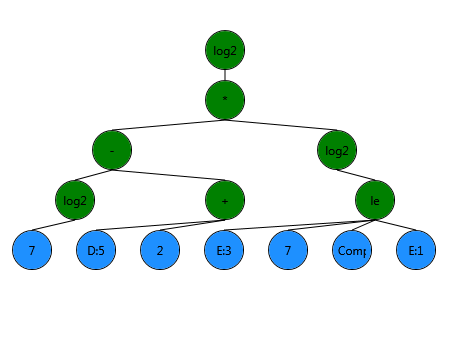
\includegraphics[width=14cm]{Images/masterThesisTree.png}
	\centering
	\caption{Example of the tree for estimating the algorithm duration on a new dataset. Terminals are blue, functions are green. The node labelled \emph{D:i} represents distance from the $i$-th nearest dataset. Similarly, the node labelled \emph{E:i} denotes error of the algorithm on the $i$-th nearest dataset. $Com$ is the complexity terminal. }
	\label{fig:masterThesisTree}	
\end{figure}

\section{Types of Metafeatures}
As devised in \cite{1976RiceAlgorithmSelectionProblem}, the extraction of metafeatures out of the problem at hand is needed for the algorithm selection problem. There are two main requirements for the metafeatures to extract -- the efficiency of the extraction and the descriptive factor of the metafeatures. The efficiency requirement is clear. The exact performance of all algorithms could be extracted as a feature but that would not give us any time savings at all. The question is what is an acceptable complexity. For instance, article \cite{metafeaturesNlogn} even suggests to restrict the complexity to $\mathcal{O}(n\log n)$ as bigger complexities are too expensive and it would be better to devote the time saved to already running some algorithms. We argue that the exact value depends on the algorithms in portfolio. With lots of algorithms and increased complexity of algorithms in portfolio, it still makes sense to compute even more expensive metafeatures. For example, if the portfolio contains NP-Complete problems, it should not be of concern to compute polynomial metafeatures. Furthermore, the suggestion is from the year 2000 and the significant increase of the CPU power and the ability to get more computational power instantly by using virtual servers in the cloud calls for not being so strict in limiting the complexity of computing the metafeatures. 

The second requirement also makes sense, as it is important to use the metafeatures that somehow help to distinguish between different algorithms. The rest is just noise and should be ignored, as even the computation of such noise can be costly.

We can distinguish metafeatures according to the nature of their computation.

The first category builds on statistic and information theory. Article \cite{MethodsForComparisonHenery1994} distinguishes three subcategories of the first category: \emph{simple}, \emph{statistical} and \emph{information-theoretic} measures. The simple measures include only very basic ones, such as the number of rows, the number of attributes or the number of integer attributes. 
Among the statistical ones, the article ranks such metafeatures as skewness, correlation, and kurtosis.
 Information-theoretic measures are motivated by information theory and are mostly appropriate for discrete attributes. The example of information-theoretic feature is \emph{entropy} of a discrete random variable: 
 \begin{equation}
 \label{equation:entropy}
H(X) = - \sum_{i}q_i\log_{2}q_i,
 \end{equation}
where $q_i$ is the probability that a variable $X$ takes on the $i$-th value. Conventionally, the entropy is converted to $\log_{2}$ as the measured value is in bits.

Authors of \cite{BrazdilMetalearning-2009} recognize two additional types of metadata -- \emph{model-based} and \emph{landmarkers}. The model-based metafeatures lies in training some sort of model on the data and take some properties of the model as metafeatures. For example, the decision tree \cite{decisionTrees} predicting the target is built. The number of nodes in the tree is introduces as a new metafeature. The landmarkers are a quick estimate of algorithm performance on the dataset. There are two ways how to do this. Either a simplified version of some algorithm is used to build the model on the whole data. For instance, the decision tree only with the top node is created and its performance evaluated on the data. Alternatively, \emph{subsampling landmarkers} use the whole algorithm on the subset of the data, which gives again the estimate.

From now on, we will treat dataset, unless stated otherwise, as the entity described by its metafeatures. We will distinguish two types of metafeatures. Propositional metafeatures (fixed size vector of metafeatures describing dataset as a whole) will be referred to in this thesis as \emph{global metafeatures}. The second type we will recognize are \emph{attribute metafeatures} -- that is the set of metafeatures extracted for each attribute in the dataset. As the number of attributes can vary per dataset, attribute metafeatures are non-propositional as we will have a vector of variable length of vectors of metafeatures. The vector of metafeatures does not have to be necessarily of a fixed size. Different types of attributes can have different types of metafeatures. We will address this in the later chapters.
The set of metafeatures will be also called metadata throughout the thesis. It can be argued that reshuffling the attributes of the datasets does not change the dataset at all. Therefore, we will consider two datasets represented by their metadata equal if and only if:
\begin{enumerate}
	\item All available global metadata are equal.
	\item All available attribute metadata are equal, or there exists a permutation (reshuffling) of attributes of the first dataset such that attribute metadata are equal after the reshuffling.
\end{enumerate}

\section{Distance Based Ranking}
\label{section:distanceBasedRanking}
In the previous sections, we have discussed the problem of algorithm ranking. The usual approach to the ranking is based on the idea that algorithms perform similarly on similar datasets. If we want to exploit this idea, we need two things -- a notion of distance between datasets and a way of calculating a ranking from the previous results on datasets similar to a dataset at hand using the distance between datasets.
In this section, we will focus on the latter and suppose that we already have the notion of distance. Throughout this thesis, when outlying the pseudocode of some algorithm, we will treat dataset distance measure as an interface taking two datasets and outputting a real number -- the measured distance between the both input datasets. This is formalized in Algorithm \ref{interface:IDatasetDistance}.

\IncMargin{1em}
\begin{algorithm}
	\SetKwData{Return}{return}
	\SetKwInOut{Input}{input}
	\SetKwInOut{Output}{output}
	\tcp{Interface for measuring distance between two datasets.}
	\Input{$a \leftarrow$ First dataset}
	\Input{$b \leftarrow$ Second dataset}
	\Output{ $d \in \mathbb{R}, d$ is a distance between $a, b$ $(d = \globalDistance(a,b))$ }
	\BlankLine
	\caption{$IDatasetDistance$: dataset distance interface}\label{interface:IDatasetDistance}
\end{algorithm}\DecMargin{1em}

This will enable us to plug different algorithms as the part of others. We will see lots of algorithms conforming to the $IDatasetDistance$ interface throughout the thesis. To avoid confusion, we will always use the symbol $\globalDistance$ when referring to the $IDatasetDistance$ interface in equations or other algorithms.

To allow for obtaining the ranking, we will define another interface called $IRanking$ -- the one that just takes a dataset and returns the ranking of algorithms to the given dataset. The interface is intentionally very generic, so we can reuse it later even with the non-distance based ranking. 

\IncMargin{1em}
\begin{algorithm}
	\SetKwData{Return}{return}
	\SetKwInOut{Input}{input}
	\SetKwInOut{Output}{output}
	\tcp{Interface for calculating the ranking to a new dataset.}
	\Input{$d \leftarrow$ dataset to rank}
	\Output{Ranking -- ordering of algorithms}
	\BlankLine
	\caption{$IRanking$: Interface for ranking calculation}\label{interface:IRanking}
\end{algorithm}\DecMargin{1em}

One could wonder how to implement $IRanking$ interface using distance based ranking. The $IRanking$ interface provides just a dataset on the input. But for the distance based ranking, at least the distance measure and other datasets need to be provided. 

To solve this, we will use a concept from functional programming.
\emph{Functional programming} \cite{functionalThinking} is a programming paradigm -- a style of building the structure and elements of computer programs -- that treats computation as the evaluation of mathematical functions. In this thesis, we will be proposing generic layered architecture of algorithms. As we want to design generic interface but the subcomponents will be initialized and parametrized differently, we will use specific functional programming construct know as partial application.

\begin{definition}
	\emph{Partial application} refers to the process of fixing a number of arguments to a function, producing another function of smaller arity. Given an integer $k$ and a function $f:X_1 \times \dots \times X_k \times \dots \times X_n \rightarrow Y$, the function $partial_k$  is defined as a function $X_1 \times \dots \times X_k \rightarrow (X_{k+1} \times \dots \times X_n \rightarrow Y)$. The $k$ is often omitted as it can be inferred from the number of input arguments.
\end{definition}

This will enable us to preinitialise some parameters and the remaining not yet assigned parameters will define the generic interface.

Because of the $partial$ application, we have an elegant way to solve the issue. We can define an interface taking all the necessary information to build up the distance based ranking and then just use $partial$ application to fix all the arguments except the dataset one. The resulting function now conforms to the $IRanking$ interface.
More formally, the $IDistanceRanking$ interface is defined in Algorithm \ref{interface:IDistanceRanking}.

\IncMargin{1em}
\begin{algorithm}
	\SetKwData{Return}{return}
	\SetKwInOut{Input}{input}
	\SetKwInOut{Output}{output}
	\tcp{Interface for calculating the ranking to a new dataset based on distance.}
		\Input{$\globalDistance \leftarrow IDatasetDistance$ - Dataset distance measure}
		\Input{exp $\leftarrow$ Previous results}
		\Input{$d \leftarrow$ Dataset to obtain ranking for}
		\Output{ Ranking -- ordering of algorithms }
	\BlankLine
	\caption{$IDistanceRanking$: Interface for distance based ranking calculation}
	\label{interface:IDistanceRanking}
\end{algorithm}\DecMargin{1em}

And the transformation of $IDistanceRanking$ interface to a more generic $IRanking$ interface is outlined in Algorithm \ref{algorithm:IDatasetRankingTransformarmation}.
\IncMargin{1em}
\begin{algorithm}
	\SetKwInOut{Input}{input}
	\SetKwInOut{Output}{output}
	\tcp{Interface for transforming $IDistanceRanking$ to $IRanking$.}
	\Input{distanceRanking $\leftarrow IDistanceRanking$ interface}
	\Input{$\globalDistance \leftarrow IDatasetDistance$ - Dataset distance measure}
	\Input{exp $\leftarrow$ Previous results}
	\Output{$IRanking$ interface}
	\BlankLine
	\Return partial(distanceRanking, $\globalDistance$, exp)\;
	\caption{Distance Ranking Transformation: transforming a $IDistanceRanking$ interface to generic $IRanking$ interface}
	\label{algorithm:IDatasetRankingTransformarmation}
\end{algorithm}\DecMargin{1em}

Now we can propose several algorithms that can be implemented to conform to the $IDistanceRanking$ interface.

The \emph{$k$-Nearest Neighbours} algorithm ($k$-NN) \cite{knn} is widely used for ranking~\cite{BrazdilMetalearning-2009}. For instance, Maratea et al. use $k$-NN in their system for solving \emph{answer set programming task} (ASP) \cite{MarateaMEASPProgressReport,MarateaMeAsp}. ASP is a declarative approach towards hard (mainly NP) search problems. The $k$-NN algorithm for ranking is aggregating previous results on the $k$ nearest neighbours identified by the distance measure to estimate the ranking. The whole method is outlined in Algorithm \ref{algo:k-nnRanking}. The complexity, provided that a distance is already precomputed, is $\mathcal{O}(n_d\log(n_d)+n_a\log(n_a))$, where $n_a$ is the number of algorithms and $n_d$ the number of datasets. If the ranking is called multiple times for different datasets, the computation of the distance could be repeated, therefore it is often useful to compute the distance outside of this function. This was the reason why we stated the complexity for already precomputed distance. This will be our case as we need lots of ranking computation to evaluate the quality of ranking algorithm. This is mainly a technicality, so for the sake of simplicity, we will not state explicitly in the algorithms that we are computing something outside of the algorithm when plugging the algorithms into one another. 

\IncMargin{1em}
\begin{algorithm}
	\SetKwInOut{Input}{input}
	\SetKwInOut{Output}{output}
	\tcp{Implementation of $IDistanceRanking$ using $k$-NN algorithm}
		\Input{$k \leftarrow$ Number of neighbours}
		\Input{$\globalDistance \leftarrow IDatasetDistance$ Dataset distance measure}
		\Input{exp $\leftarrow$ Previous results}
		\Input{$d$ $\leftarrow$ Dataset to obtain ranking for}
		\Output{ Ranking }
	\BlankLine	
	distances $\leftarrow []$\;
		\ForEach{\upshape dataset $\in$ exp.datasets}{
			current\_distance $\leftarrow \globalDistance(d,\text{ dataset})$\;
			distances $\mathrel{+}=  [(\text{dataset, current\_distance})]$\;
		}
		distances $\leftarrow$ sort(distances, (dataset, distance):distance)\;
		neighbours $\leftarrow$ distances$[:k]$\;
		\ForEach{\upshape algorithm $\in$ exp.algorithms}{			
				$r_{\text{algorithm}} \leftarrow 0$\;
		}
		\ForEach{\upshape neighbour $\in$ neighbours}{
					\ForEach{\upshape algorithm $\in$ exp.algorithms}{			
				$r_{\text{algorithm}} \mathrel{+}=$ exp.rank(neighbour, algorithms)\;
			}
		}		
	$R \leftarrow [1, \dots$ len(exp.algorithms)$]$\;
	$R \leftarrow$ sort($R$, algorithm: $r_{\text{algorithm}}$)\;
	\Return $R$\;
	\caption{$K$-NN Ranking: $k$-NN based implementation of $IRanking$.}
	\label{algo:k-nnRanking}
\end{algorithm}\DecMargin{1em}

The $k$-NN algorithm can be also modified in such a way to involve the weights into computation, so that closer neighbours have bigger influence on the final result \cite{weightedKnn}.
The number of neighbours -- $k$ -- is the crucial parameter of the whole algorithm. Setting of $k$ to 1 or similarly low values usually results in overfitting and corresponding bad generalization abilities of the model. On the other hand, high values of $k$ defeat the purpose of the local neighbourhood and tend to have lower performance as the information from the distant regions affect the decision process. To address this, there has been also some additional modifications proposed to the $k$-NN algorithm. The \emph{G-means} algorithm \cite{gmeans} enhances the original algorithm by automatically setting the number of neighbours. The G-means is based on a statistical test for the hypothesis that a subset of data follows a Gaussian distribution. The G-means runs $k$-means with increasing $k$ in a hierarchical fashion until the test accepts the hypothesis that the data assigned to each $k$-means centre are Gaussian. Two key advantages are that the hypothesis test does not limit the covariance of the data and does not compute a full covariance matrix. The $G$-means algorithm was used for algorithm selection by authors of \emph{Autofolio} \cite{FrankHutterAutomaticallyConfiguredAlgorithmSelector}. The G-means is used together with other algorithms for automatic selection of parameters to solve some artificial intelligence problem at hand (e.g. \emph{satisfiability} (SAT), \emph{constraint satisfaction programming} (CSP) or \emph{quantified boolean formula} (QBF)). In \cite{algorithmSelectionAndScheduling}, the G-means is used in algorithm portfolio selection of the SAT solvers. Motivated by the observation that solvers have complementary strengths and therefore exhibit incomparable behaviour on different problem instances, algorithm portfolios run multiple solvers in parallel or select one solver, based on the features of a given instance. 

In \cite{jaICMLA2013}, we investigated the possibility of distance based ranking using clustering constructed from the training set. In our case, the clustering  was a result of an \emph{agglomerative clustering algorithm} \cite{hierarchicalClustering}. The advantage of this clustering method is that it does not require creation of centroids as in the case of other methods. Compared to the $k$-NN algorithm, the neighbourhood does not have a fixed size but rather a variable size depending on the cluster method.

The bottom up method was chosen because it is faster than the top down method. The question arises which criterion of clusters’ distance to use. We have adopted \emph{Unweighted Pair Group Method with Arithmetic Mean} (UPGMA), or average linkage clustering \cite{hierarchicalClustering}, which is used in various applications~\cite{hierarchicalClusteringApplications}.

In our experiments, ranking was constructed the same way as in the $k$-NN ranking algorithm with the exceptions that the nearest neighbours of the given dataset were selected according to the nearest cluster, given metric and UPGMA method. In the experiments, we have used the results of 8 \emph{Weka} \cite{weka} algorithms on the 85 \emph{UCI} (Dataset Repository of University of California, Irvine) \cite{uci} datasets. The datasets were divided into the training and testing set with the ratio of 2:1. We have tested various distance metric to estimate the algorithm performance. Results indicated that such hierarchical clustering can be successfully used for metalearning. The best dendrogram of the best cluster is shown in Figure~\ref{fig:dendrogram}. 

\begin{figure}
	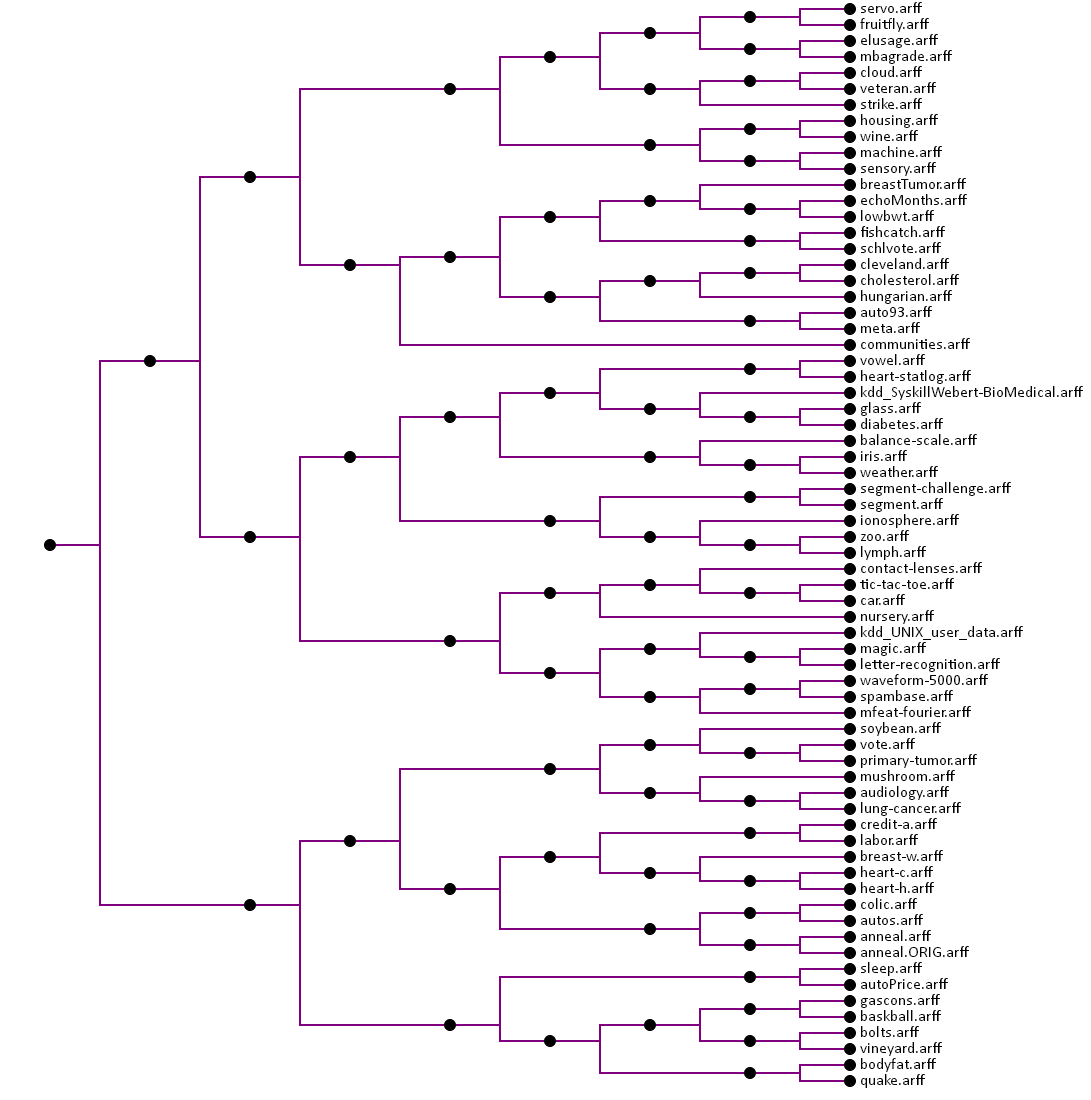
\includegraphics[width=14cm]{Images/tree.png}
	\centering
		\caption{The dendrogram as a result of the agglomerative clustering \cite{jaICMLA2013}. Datasets are assigned to clusters according to their similarity.}
		\label{fig:dendrogram}	
\end{figure} 
 
\section{Assessing the Ranking Quality}
\label{section:rankingQuality}
In this section, we describe techniques to asses the quality of some method for predicting the ranking of algorithms. 
Given some $IRanking$ interface implementation and a new dataset $d$, the \emph{Spearman's rank correlation coefficient} can be used to asses the accuracy of the ranking method:
\begin{equation}
\label{eq:spearman}
r_s^d=1-\frac{6\sum_{i=1}^{n}(R^{'d}_i-R^d_i)^2}{n^3-n},
\end{equation}
where $n$ is the number of models, $R^d_i$ is the actual rank of model $i$ on dataset $d$ and $R^{'d}_i$ is the predicted rank of model $i$ on dataset $d$. The Spearman's rank correlation coefficient has some interesting properties. The range of the coefficient is normalized to the interval $\langle-1,1\rangle$, where 1 is a perfect match, -1 is a perfect mismatch and 0 indicates results as good as random guessing.
Equation \ref{eq:spearman} gives us the means of measuring ranking quality for a single dataset. If the aim is to measure the quality over all datasets, it is possible to take Spearman's rank correlation coefficient averaged over all datasets: 
\begin{equation}
\label{eq:averageSpearman}
r_s=\frac{\sum_{d=1}^{n}r^d_s}{n},
\end{equation}
where $n$ is the number of datasets and $r^d_s$ is the Spearman's rank correlation coefficient computed for dataset $d$.

The whole ranking quality assessment is summarized in Algorithm \ref{algo:rankingQualityEvaluation}.
\IncMargin{1em}
\begin{algorithm}
	\SetKwInOut{Input}{input}\SetKwInOut{Output}{output}
	\tcp{Pseudocode for ranking prediction quality assessment using dataset distance function.}
	\Input{datasets $\leftarrow$ List of datasets}
	\Input{predictor $\leftarrow IRanking$ Ranking predictor}
	\Input{results $\leftarrow$ Results of algorithms on datasets indexed by datasets}
	\Input{algorithms $\leftarrow$ List of algorithms}
	\Output{Ranking Prediction Quality Assessment}
	\BlankLine
	$r_s\leftarrow$ 0\;
	$n \leftarrow$ len(algorithms)\;
	\ForEach{\upshape dataset $\in$ datasets}{
		remaining $\leftarrow$ datasets $\setminus$ dataset\;
		$R^{\text{dataset}} \leftarrow$ predictor(dataset, remaining, results, algorithms)\;		
		$r_s^{\text{dataset}} \leftarrow  1-\cfrac{6\sum_{i=1}^{n}(R^{\text{dataset}'}_i-R^{\text{dataset}}_i)^2}{n^3-n}$\;
		$r_s \leftarrow r_s+\cfrac{r_s^{\text{dataset}}}{n}$\;
	}
	\Return $r_s$\;
	\caption{Ranking Quality Assessment}\label{algo:rankingQualityEvaluation}
\end{algorithm}\DecMargin{1em}

Basically, the algorithm for each dataset estimates the ranking of algorithms by using $IRanking$ interface. The quality of rankings is measured using Equation \ref{eq:averageSpearman}. Provided the predictions are already precomputed, we get a complexity of the quality evaluation: $$\mathcal{O}(n_dn_a),$$
where $n_d$ is the number of datasets and $n_a$ is the number of algorithms.

\section{Ranking Baseline}
\label{section:baseline}
Algorithm \ref{algo:rankingQualityEvaluation} can give us a good estimate of how good our model is compared to random guessing. However, there may be trivial methods that are very easy to implement, yet they exhibit a relatively good performance. Such trivial algorithms are often referred to as \emph{baseline} algorithms. Their output is usually based on some statistical knowledge about the data and is calculated using the most frequent values. Complex algorithms should outperform baseline algorithms, otherwise there is no need for the extra complexity.
In the classification tasks, the baseline usually outputs the most frequent class. In the regression task, the median or average of the target values is usually returned by the baseline algorithm. We can also define a baseline algorithm for the ranking task. The baseline algorithm can predict the ranking results based on algorithm's average rank on all datasets present in the metaknowledge base. If one algorithm is the best in average on all datasets, baseline algorithm will just assign the first rank to this algorithm. Again, we will design the baseline algorithm with the $IRanking$ interface in mind. To calculate the ranking, baseline needs the information about the average ranking. One could be tempted to use again the trick with the $partial$ function. In this case this would be a mistake, as that would result in recalculating the average ranking for each call to the interface. Instead, we will create a function that takes previous results as an input, calculates average ranking, and then returns a function conforming to the $IRanking$ interface. Such course is outlined in Algorithm \ref{algo:rankingBaseline}. The complexity of resulting $IRanking$ is constant. To build up the distance, one has to do $$\mathcal{O}(n_dn_a + n_a\log(n_a))$$
steps, where $n_d$ is the number of datasets and $n_a$ is the number of algorithms. The term $(n_dn_a)$ represents the cost of two inner loops, the term $n_a\log(n_a)$ is for sorting the rankings.
\begin{algorithm}
	\SetKwInOut{Input}{input}
	\SetKwInOut{Output}{output}
	\tcp{Pseudocode for building the ranking baseline model.}
	\Input{datasets $\leftarrow$ List of datasets}
	\Input{algorithms $\leftarrow$ List of machine learning algorithms}
	\Input{results $\leftarrow$ Results of algorithms on datasets indexed by datasets}
	\Output{$IRanking$ interface}
	\BlankLine
	averageRanking $\leftarrow []$\;
	occurrences $\leftarrow []$\;
	\ForEach{\upshape algorithm $\in$ algorithms}{
		averageRanking[algorithm]$\leftarrow 0$\;
		occurrences[algorithm] $\leftarrow 0$\;
	} 
	\ForEach{\upshape dataset $\in$ datasets}{
		resultsOnDataset $\leftarrow$ results[dataset]\;
		\ForEach{\upshape algorithm $\in$ algorithms}{
			\If{\upshape algorithm $\in$ resultsOnDataset}
			{
				occurrences[algorithm]$\mathrel{+}\mathrel{+}$\;
				currentRank $\leftarrow \cfrac{\text{resultsOnDataset[algorithm]}}{\text{len(resultsOnDataset)}}$\;
				averageRanking[algorithm]$\mathrel{+}=$ currentRank\;
			}
		}
	}
	averageRankingWithAlgorithm $\leftarrow$ zip(averageRanking,algorithms)\;
	averageRankingWithAlgorithm $\leftarrow$ map(averageRankingWithAlgorithm,$\lambda(x,y)\rightarrow \cfrac{x}{occurrences[y]},y)$\;
	averageRankingWithAlgorithm$\leftarrow$ sort(averageRankingWithAlgorithm,$(x,y):x$)\;
	\Return $\lambda(x) \rightarrow $ averageRankingWithAlgorithm\;
	\caption{Ranking Baseline}\label{algo:rankingBaseline}
\end{algorithm}\DecMargin{1em}

\section{Performance Indicators}
In the previous sections, we have discussed the metatarget and ranking in particular. We did not discuss what should be the performance indicator defining the metatarget. It can be any of the performance measures mentioned in Section \ref{section:mlTasks} or a combination of them. The time complexity can also be predicted or time can be included into the performance consideration. This is useful when good and fast learning algorithms are preferred.  The time is especially crucial when the resources are scarce or expensive.

The time cost value of following some ranking strategy is captured by the \emph{top-$N$} evaluation \cite{topNEvaluation}. The $N$ is a parameter that determines how many best algorithms will be tried on some dataset. Different settings of $N$ can be consequently simulated, and we can observe how the accuracy of the best model improved compared to the time cost associated with the increase of $N$.

The top-$N$ strategy has a disadvantage that it is unable to leverage what is learned from previous evaluations.
Alternatively, we can tackle this issue with a strategy called \emph{active testing} \cite{activeTesting}. It proceeds in a tournament-style fashion, in each round selecting and testing the algorithm that is most likely to outperform the best algorithm of the previous round on the new dataset. The next contender is selected based on the concept of \emph{relative landmarkers} \cite{relativeLandmarkers}. These landmarkers estimate the relative probability that a particular algorithm will outperform the current best candidate. The \emph{cross-validation} \cite{aima3ed} of the new contender is performed. The result is added to the relative landmarkers and the contender replaces the current best algorithm if the cross-validation result is better or ties the result of current best algorithm.

One approach of combining time and accuracy was proposed by Brazdil et al. \cite{Brazdil00zoomedranking}. The $k$-Nearest Neighbours algorithm \cite{knn} with a distance function based on a set of statistical, information theoretic, and other dataset characterization measures is employed in order to identify the set of similar already computed tasks. For the ranking phase, the adjusted ratio of ratios ranking method is presented, which processes performance information based on accuracy and time.

The relevance of the processed dataset $d_i$ to the dataset $d_j$ at hand is defined in terms of similarity between them, according to metafeatures. It is given by a metric (or a distance function):
\begin{equation}
\globalDistance\left(d_i,d_j\right)=\sum_{x} \sigma\left(v_{x,d_i},v_{x,d_j} \right),
\end{equation}
where $d_{i}$ and $d_j$ are datasets, $v_{x,d_i}$ is the value of metafeature $x$ for dataset $d_i$, and $\sigma\left(v_{x,d_i},v_{x,d_j} \right)$ is the distance between the values of metafeature $x$ for datasets $d_{i}$ and $d_j$. All metafeatures are normalized.

The $k$-Nearest Neighbours algorithm is then used to identify the $k$ cases nearest to the dataset at hand.

The \emph{adjusted ratio of ratios} uses information about accuracy and execution time to rank the given classification algorithms. It is computed by means of the auxiliary term ${ARR}_{a_p,a_q}^{d_i}$ defined as:

\begin{equation}
{ARR}_{a_p,a_q}^{d_i}=\frac{\frac{SR_{a_p}^{d_i}}{SR_{a_q}^{d_i}}}{1+\frac{\log{\left(\frac{T_{a_p}^{d_i}}{T_{a_q}^{d_i}}\right)}}{K_T}},
\end{equation}
where $SR_{a_p}^{d_i}$ and $T_{a_p}^{d_i}$ are the success rate and duration of algorithm $a_p$ on the dataset $d_i$, and $K_T$ is a user-defined value that represents the amount of accuracy the user is willing to trade for a 10 times speed-up or slowdown. For example, $K_T$ = 10\% means that the user is willing to trade 10\% of accuracy for 10 times speed-up. 

Finally, the overall mean adjusted ratio of ratios for each algorithm is derived:
\begin{equation}
{ARR}_{a_p}=\frac{1}{m-1}\left(\sum\nolimits_{a_q} \frac{\sum\nolimits_{d_i} {{ARR}_{a_p,a_q}^{d_i}}}{n} \right),
\end{equation}
where $m$ is the number of algorithms and $n$ is the number of datasets. The ranking is based on this measure.
Authors of \cite{brazdilArrCorrected} including one of original authors of $ARR$ looks into the $ARR$ measure and argue that $ARR$ should be monotonically increasing Higher success rate ratios should lead to higher values of ARR and, similarly, higher time ratios should lead to lower values of ARR. Experiments were proposed to verify this property on data. The $\frac{SR_{a_p}^{d_i}}{SR_{a_q}^{d_i}}$ was fixed to 1, the time ratio was sampled from very small $2^{-20}$ to very high values $2^{20}$ and three different values of $K_T$ were used ($0.2, 0.3, 0.7$). The resulting ARR function was not monotonic and was even approaching infinity at some point. In general, this can lead to incorrect rankings provided by the metalearner and can affect the evaluation results. Authors proposed a solution that addresses this issue by changing the re-sampling used in $ARR$. The updated formula $A3R$ was proposed:
\begin{equation}
{A3R}_{a_p,a_q}^{d_i}=\frac{\frac{SR_{a_p}^{d_i}}{SR_{a_q}^{d_i}}}{\sqrt[n]{\frac{T_{a_p}^{d_i}}{T_{a_q}^{d_i}}}},
\end{equation}
where $n$ is a user defined constant representing the importance of time.

The $A3N$ is used in \cite{brazdil_a3rExperiments} as a performance indicator. The paper proposes several modification to active testing strategy \cite{activeTesting}. The first approach uses faster sample-based tests to identify competitive algorithms. The second modification lies in argument that full cross-validation test is not necessary to estimate the next candidate. Instead, the test is performed on a smaller sample of the new dataset. This is motivated by the fact that a sample-based test is much faster than a full cross-validation test. The full cross-validation test is carried out only if a candidate algorithm beats the currently best algorithm on the sample-based test.

\section{Systems for Algorithm Recommendation}
\label{section:recommenderSystems}
Having a viable framework for metalearning is only one side of a coin. The actual systems built for metalearning are called \emph{recommendation system}. Their goal is to allow for a trade-off between human time and machine time. They can also provide the power of machine learning algorithms to the non-expert users, even to those with limited computer knowledge. There are many scenarios for such systems.

\emph{Auto-weka} \cite{autoWeka} is a system integrating into the Weka toolkit \cite{weka} and it is able to perform model selection, and autotune model parameters. It employs the \emph{Sequential Model-based Algorithm Configuration algorithm} (SMAC) \cite{autoWekaSMAC}. SMAC supports a variety of models of the type $p(c| \lambda)$ to capture the dependence of the loss function $c$ on hyper-parameters $\lambda$, including approximate Gaussian processes~\cite{gaussianProcesses} and random forests \cite{randomForests}. 

Autofolio \cite{FrankHutterAutomaticallyConfiguredAlgorithmSelector} combines SMAC with algorithm selection framework claspfolio2~\cite{claspfolio2}. \emph{Claspfolio2} is a flexible framework that provides functionality to train and assess the performance of different algorithm selection techniques. The extensibility is the main advantage and it provides an unified framework for algorithm selection problem. The overview of all components is in Figure \ref{fig:claspfolio2}. The scheduling system is also integrated.

\begin{figure}
	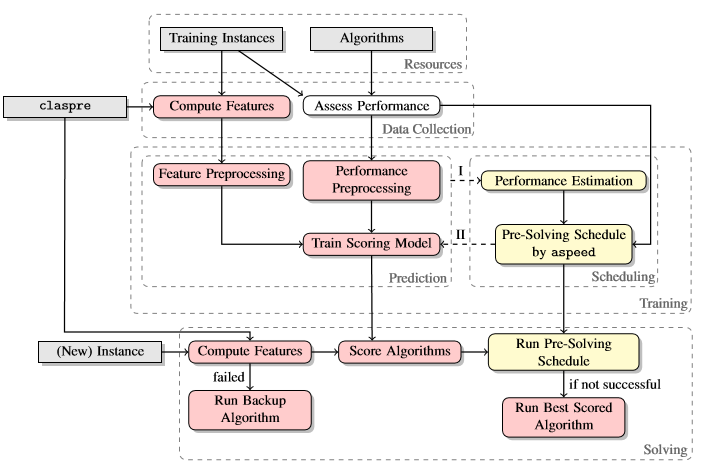
\includegraphics[width=14cm]{Images/claspfolioSchema.png}
	\centering
	\caption{Overview of claspfolio2 framework \cite{claspfolio2}.}
	\label{fig:claspfolio2}	
\end{figure}

Our recommendation system called \emph{Pikater} \cite{jaPikater, icmlaHawaii, wiat11, KazikIAENG} is implemented using \emph{multi-agent systems} (MAS). To be precise, the multi-agent framework \emph{JADE} \cite{JADE} is used as a platform of the system. The extensibility is assured by the use of the structured ontology language and following the \emph{Foundation for Intelligent Physical Agents} (FIPA) \cite{FIPA} international standards of agents' communication. The following basic scenarios have been considered.
\begin{itemize}
	\item In the most simple case, the user knows which method and what parameters of that method they would like to use.
	\item In the second scenario, the user knows what method to use but does not know how to set its parameters. The system is able to search the parameter space of the method and find a setting that provides good results. 
	\item In the third case, the user does not even know what method to use and lets the system decide by itself. In this case, the system recommends the best possible method or provides a ranking of the methods based on predicted errors and duration.
\end{itemize}
These simple scenarios can be extended into more complex ones. For instance, it is also possible to combine the recommendation of the best method with parameter space search, when the system recommends an interval of the parameter’s values. As a positive side effect, the metaknowledge base for metalearning purposes is being built up by each experiment. 

In order to effectively design our system, we have chosen the organization-centred formalism \emph{AGR} (Agent-Group-Role) \cite{agr}. The role is a set of capabilities and responsibilities that the agent accepts by handling the role. Group — the building block of a MAS — is a set of agents with allowed roles and interactions, defined by a group structure. The multi-agent system then consists of multiple groups which can overlap, as agents can belong to more than one group. In this formalism, we abstract from the algorithmic details and inner logic of the agents in the MAS. Authors of \cite{KazikIAENG} used the ontological formalism of \emph{OWL-DL} \cite{pelletOwlDl} to describe the organizational model of Pikater. The following group structures were defined according to the aforementioned scenarios: administrative group structure, computational group structure, search group structure, recommendation group structure, data group structure, and data-management group structure. Our MAS is composed of groups that are instances of these group structures. The architecture is depicted in Figure \ref{fig:pikaterArchitecture}.


\begin{figure}
	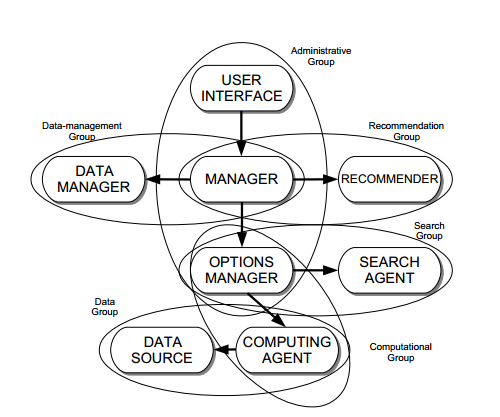
\includegraphics[width=14cm]{Images/pikaterArchitecture.png}
	\centering
	\caption{Overview of Agent-Group-Role model of our recommendation system Pikater \cite{jaPikater}.}
	\label{fig:pikaterArchitecture}	
\end{figure}

The MAS-based solution allows for a flexibility in choice of the parameter space search algorithms, each of these is encapsulated in a search agent. General tabulation, random search, simulated annealing \cite{aima3ed}, or parallel methods, such as genetic algorithms, are implemented in our system. Another great benefit of the agent-based approach is the natural capability to parallelly execute multiple computations with various parameters. This significantly decreases the time needed for the execution of the parameter space search process. One of essential features of our MAS is its capability of recommending a suitable computational method for a new dataset, according to datasets similarity and previously gathered experience. The choice of the similar dataset(s) is based on various previously proposed metrics \cite{hierarchicalClustering}, which measure the similarity of their metadata. Our database contains over 600,000 records, that are used to suggest the proper method (including its parameters) and estimate its performance on a new dataset. The latest version of our MAS contains the following types of recommenders, which differ in the metric used and in the number of recommended methods they provide:
\begin{itemize}
	\item Basic recommender chooses a method based on the single closest dataset using the unweighted metadata metric.
	\item Clustering Based Classification \cite{jaICMLA2013} chooses the whole cluster of similar datasets and the corresponding methods, using different sets of metadata features.
	\item Evolutionary Optimized Recommenders are similar to the two above described recommender types, using different weighted metrics, optimized by an evolutionary algorithm.
	\item Interval Recommender recommends intervals of suitable parameter values and leaves their fine-tuning to the parameter space search methods.
\end{itemize}
Another functionality of our system is a multi-objective optimization of data mining configurations. To test this, the search algorithm is employed in order to find beneficial combinations of pre-processing and machine learning methods to the presented data. The minimization is performed in error-rate as well as run-time criteria \cite{Kazik2015}.

\section{Related Work}
In this section, we further review some of the literature related to metalearning. Authors of \cite{KazikPesk} define the distance between datasets based on the following metadata:
\begin{itemize}
	\renewcommand{\labelitemi}{$\bullet$}
	\item \textit{Number of attributes} in data,
	\item \textit{Number of instances},
	\item \textit{Data type} (Relates to all values of all attributes in the dataset. Four categories of data are considered -- categorical, integer, real, or multivariate -- different attributes are of different types),
	\item \textit{Default task type} (Set by the user, the most common types are classification and regression),
	\item \textit{Missing values} (Flag whether data contains unknown or unspecified values).
	\end{itemize}
	The following metric is defined between two tasks based on their metadata:
	\begin{equation}
	\globalDistance(dataset_1,dataset_2) = \sum_{i=1}^{n}w_i\sigma_i(dataset_1[i], dataset_2[i]),
	\end{equation}
	where $dataset_j[i]$ is the $i$-th metadata of the $j$-th dataset, $w_i$ is the weight of the $i$-th metafeature and $\sigma_i$ is the distance on the $i$-th metafeature defined by the type of the $i$-th metafeature. For categorical or boolean type the $d_i$ is 0 if the value matches, otherwise 0. For the numerical types of metadata the normalized difference between their value is taken as a distance.
	
	There is also a work by Graff and Poli~\cite{PoliPerformanceModels} based
	on evolutionary program induction. They use (among other techniques) genetic
	programming to predict the performance of various algorithms, such as neural networks,
	to solve given tasks. 
	
	Kordík and Černý \cite{kordikMetalearningTemplates} propose the evolution of so called \emph{templates}. Templates specify the workflow to produce a model and are the collection of ensembling algorithms, modelling and classification algorithms combined in a hierarchical manner. These templates are evolved using genetic algorithms in order to produce the best results. The similarity of templates can be used as a landmarker metadata.	
	
	Misir and Sebag \cite{MisirAlgorithmSelectionAsCollaborativeFiltering} used a completely different approach.
	They formulated a more general problem of algorithm selection as a
	\emph{collaborative filtering problem} \cite{CollaborativeFilteringSurvey}. In this case,  instead of talking about the
	selection of methods for given dataset, we can imagine that the various methods
	rate the datasets based on their performance. The methods prefer the datasets,
	on which they have better performance. Interestingly, such an approach does not
	require any metadata, it is possible to run a few of the methods, find their
	performance and use this information to recommend better methods. However, if
	some metadata are available, they can be used instead of running the methods.
	
	\section{Principal Component Analysis}
	\label{section:pca}
	In this section, the \emph{Principal Component Analysis} (PCA) \cite{pca} method is described, as it will be used further in the thesis.
	
	PCA is an orthogonal linear transformation to a new coordinate system such that the greatest variance by some projection of the data comes to lie on the first coordinate (called the first principal component), the second greatest variance on the second coordinate, and so on. 
	
	%http://www.cs.otago.ac.nz/cosc453/student_tutorials/principal_components.pdf
	Given some dataset, we begin the PCA by subtracting the mean of each dimension from the dimension itself. We then calculate the covariance matrix of the data. The next step is calculation of the eigenvectors and eigenvalues of the covariance matrix. This is possible since the covariance matrix is square. This gives us the components. If we order the eigenvectors by eigenvalues, we get the ordering by significance. We can reduce the dimension by ignoring the components with less significance.
	Suppose we have decided to keep $k$ components. Now we form the $FeatureVector$ as follows:
	\begin{equation*}
	FeatureVector = (eigenvector_1 \dots eigenvector_k).
	\end{equation*}
	The $FeatureVector$  is a matrix with eigenvectors as columns.
	We get the data in the new coordinate system by the following operation:
	
	\begin{equation*}
	NewCoordinates = FeatureVector^T \times DataAdjustedByMeans^T,
	\end{equation*}
	where $DataAdjustedByMeans$ are the original data with the means subtracted.
	
	It is also possible to calculate points back and forth between the original coordinate systems and the new one. This is useful when we add some new data (regardless of the encoding).
	
	PCA is often used for visualizing multi-dimensional data, as it can be used to reduce the number of dimension to two or three dimensions.




%- princip je využití atributů
%- kernely a kus z related work
% algoritmus
%- vlastnosti - věty o metrikách - možná zvláštni kapitola

\chapter{Global Distance}
\label{chapter:globalDistance}
In the previous chapter, the concept of distances between datasets was introduced. In this chapter, we will discuss what are the properties of good distance measures in general. We will define a \emph{metric} and \emph{metric spaces}. We will also define a concept of \emph{norms}, which can be intuitively used to form a metric. We give a few examples of norms -- \emph{$p$-norms} and their weighted counterparts, and we outline a recognized fact that $p$-norms are indeed a norms using the \emph{H\"older's} and \emph{Minkowski's} inequalities. We summarize a few well known theorems about metric spaces -- that it is possible to rescale the metric space without violating the metrics axioms and that the sum of metric is also a metric. These facts will be useful in the chapters to follow. We move back to dataset distance measures and define a class of such distance measures using the global metafeatures. We will show that if the distance is based on weighted $p$-norms, then the resulting dataset distance is a metric. 

\section{Metric Spaces}
In this section, we will define metric, metric spaces and norms. We will also present few examples of the metrics.

\begin{definition}
	\label{definition:metric}
	A \emph{metric} on a set $X$ is a function (called the distance function or simply distance)
	\begin{equation}
	d : X \times X \rightarrow [0,\infty),
	\end{equation}
	and for all x, y, z in X, the following conditions are satisfied:
	\begin{enumerate}
		\item $d(x,y) \geq 0$ (\emph{non-negativity}).
		\item $d(x,y) = 0 \Leftrightarrow x = y$ (\emph{coincidence axiom}).
		\item $d(x,y) = d(y,x)$ (\emph{symmetry}).
		\item $d(x,z) \leq d(x,y) + d(y,z)$ (\emph{triangle inequality}).
	\end{enumerate}	
\end{definition}

\begin{definition}
	\emph{Metric space} is a tuple $(X,d),$ where $M$ is a set and $d$ is a metric on $M$.
\end{definition}

The first condition of Definition \ref{definition:metric} is sometimes omitted as the following holds:
\begin{theorem}
	\label{theorem:metricaxiom1redundant}
	Metric conditions 2, 3 and 4 imply condition 1.
	\begin{proof}
		\begin{align}
		d(x,x) &\le d(x,y)+d(y,x) & | & triangle \: inequality \label{eq:metricStep1} \\
		d(x,x) &\le 2d(x,y) & | &  symmetry, \ref{eq:metricStep1} \label{eq:metricStep2}\\
		0 &\le 2d(x,y) & | &  coincidence, \ref{eq:metricStep2} \label{eq:metricStep3} \\
		d(x,y) &\ge 0 & | &  \ref{eq:metricStep3}
		\end{align}
	\end{proof}
\end{theorem}
In this thesis, we will prefer to use all four conditions, as it will later enable us to relax the definition of a metric a little bit, and propose additional algorithms for solving the algorithm ranking task.

\subsection{Metric Examples}
In this section, we will list few metric examples that will be later reused further in the thesis.

\begin{theorem}
	\label{theorem:discretemetric}
	Let $M = \mathbb{R}^n$ and $x,y \in M$. Then function defined as
	\begin{equation}
	d(x,y)=
	\begin{cases}
	0; \text{ if } x = y, \\
	1; \text{ otherwise}.
	\end{cases}
	\end{equation}
	is a metric on $M$.	
\end{theorem}
\begin{definition}
	We will denote the metric from Theorem \ref{theorem:discretemetric} as the \emph{discrete metric}. It can be easily verified that the discrete metric is indeed a metric.
\end{definition}

\begin{definition}
	Let $V$ be a vector space over $\mathbb{F}$ (with $\mathbb{F} = \mathbb{R}$ or $\mathbb{F} = \mathbb{C}$) and $N:V \rightarrow \mathbb{R}$ a map such that, writing $N(u)=||u||$, the following results hold:
	\begin{enumerate}
		\item $\forall u \in V: ||u||\ge 0$ (\emph{non-negativity}).
		\item $\forall u \in V: ||u|| = 0 \iff u = \overrightarrow{0}$ (\emph{separates points}).
		\item $\forall \lambda \in \mathbb{F}, \forall u \in V: ||\lambda u||=|\lambda|||u||$ (\emph{absolute scalability}).
		\item $\forall u,v \in V: ||u||+||v|| \ge ||u+v||$ (\emph{triangle inequality}).
	\end{enumerate}
	Then we call $||\cdot||$ a \emph{norm} and say that $(V, ||\cdot||)$ is a \emph{normed vector space}.
\end{definition}
Normed vector space can be easily transformed into a metric space:
%http://web.utk.edu/~utkreu/docs/GTmini1.pdf
\begin{theorem}
	\label{theorem:metricfromnorm}
	Let  $(V, ||\cdot||)$ be a normed vector space. Then function $d: V^2 \rightarrow \mathbb{R}$ defined as:
	\begin{equation}
	d(u,v) = ||u-v||
	\end{equation}
	is a metric on $V$. Consequently, the tuple $(V, d)$ is a metric space.
	\begin{proof}
		We will split the proof according to the different metric axioms.
		\begin{enumerate}		
			\item We will begin with proving the coincidence axiom:	
			$$0 = d(v,w) \iff ||v-w|| =0 \iff v - w = \overrightarrow{0} \iff v = w.$$
			\item Symmetry can be derived using the second axiom of the norm:
			\begin{equation}
			d(v,w)=||v-w||=|-1|||w-v||=||v-w||=d(w,v).
			\end{equation}
			\item A proof of triangle inequality uses the fourth norm property:
			\begin{align}
			d(v,w) &= ||v-w||=||(v-u)+(u-w)|| \le \\
			& \le ||(v-u)||+||(u-w)||=d(v,u)+d(u,w).
			\end{align}
			\item 	The first metric axiom is implied by Theorem \ref{theorem:metricaxiom1redundant}. 	 
		\end{enumerate}
	As we have proven every metric axiom, we can conclude the proof.
	\end{proof}
\end{theorem}
\begin{definition}
	For $p \ge 1$, the \emph{p-norm} of $x \in \mathbb{R}^n$ is defined as $$||x||_p = {\left( \sum_{i=1}^{n}|x_i|^p \right)}^{1/p}.$$
\end{definition}

To show that the $p$-norm is formally a norm, we will first state two theorems -- H\"older's Inequality and Minkowski's Inequality.

\begin{theorem}[H\"older's Inequality]
	\label{theorem:holdersInequality}
	Let $a,b$ be vectors in $\mathbb{R}^n$ and $p,q > 1, p,q \in \mathbb{R}$ satisfy $\frac{1}{p}+\frac{1}{q}=1$. Then
	\begin{equation}
	\sum_{i=1}^{n}|a_ib_i| \le {\left( \sum_{i=1}^{n}|a_i|^p \right)}^{1/p} {\left( \sum_{i=1}^{n}|b_i|^q \right)}^{1/q}.
	\end{equation}
	\begin{proof}
		We will divide the proof into two steps. In the first step, we will prove an auxiliary claim that will be used in the step 2 to finally prove the desired inequality.
		\begin{itemize}
			\item Step 1.		
			We shall show that if $x,y > 0, x,y \in \mathbb{R}$ and $0 < \lambda < 1, \lambda \in \mathbb{R}$ then
			\begin{equation}
			x^{\lambda}y^{1-\lambda} \le \lambda x + (1-\lambda)y.
			\end{equation}
			Set $t=\frac{x}{y}$. Then after dividing both sides of the equation by $y$, we get the equivalent equation to prove $t^{\lambda} \le \lambda t + (1-\lambda)$.
			
			Set $\phi(t)=\lambda t + (1-\lambda)-t^{\lambda}$. Then we need to show that $\phi(t) \ge 0$. We will investigate the first derivative of $\phi$: $\phi'(t)=\lambda - \lambda t^{\lambda-1}=\lambda(1-t^{\lambda-1})$, so
			\begin{equation}
			\phi'(t)=
			\begin{cases}
			< 0; \text{ if } t < 1, \\
			= 0; \text{ if } t = 1, \\
			> 0; \text{ otherwise}.
			\end{cases}
			\end{equation}
			Since $\phi(1)=0$, according to the derivatives this must be a global minimum of the function and therefore the step 1 is concluded.
			\item Step 2. Let us define $A_i$ and $B_i$ as
			\begin{equation}
			A_i={\frac{|a_i|^p}{\sum_{i=1}^{n}|a_i|^p}},
			B_i = {\frac{|b_i|^q}{\sum_{i=1}^{n}|b_i|^q}}.
			\end{equation}
			Let $\lambda = \frac{1}{p}$. Then, by Step 1, 
			\begin{equation}
			A_i^{1/p}B_i^{1/q} \le \frac{A_i}{p}+\frac{B_i}{q}
			\end{equation}
			as $\frac{1}{q}=1-\frac{1}{p}$. By fully expanding $A_i$ and $B_i$, we obtain
			\begin{equation}
			{\frac{|a_i|}{{\left( \sum_{i=1}^{n}|a_i|^p \right)^{1/p}}}}
			{\frac{|b_i|}{{\left( \sum_{i=1}^{n}|b_i|^q \right)^{1/q}}}}
			\le
			\frac{1}{p}{\frac{|a_i|^p}{\sum_{i=1}^{n}|a_i|^p}}
			+ \frac{1}{q}{\frac{|b_i|^q}{\sum_{i=1}^{n}|b_i|^q}}.
			\end{equation}
			By summing above equation over $1, \dots ,n$ we obtain
			\begin{equation}
			{\frac{\sum_{i=1}^{n}|a_i||b_i|}{\left( \sum_{i=1}^{n} |a_i|^p \right)^{1/p}
					\left( \sum_{i=1}^{n} |b_i|^q \right)^{1/q}		
				}}
				\le \frac{1}{p}+ \frac{1}{q}=1.
				\end{equation}
				Multiplying both sides by $\left( \sum_{i=1}^{n} |a_i|^p \right)^{1/p}
				\left( \sum_{i=1}^{n} |b_i|^q \right)^{1/q}$ concludes the proof of the H\"older's Inequality.
			\end{itemize}
		\end{proof}
	\end{theorem}
	
	\begin{theorem}[Minkowski's Inequality]
		\label{theorem:minkowskiInequality}
		Let $a,b$ be vectors in $\mathbb{R}^n$ and $p \ge 1, p \in \mathbb{N}$. Then
		\begin{equation}
		{\left( \sum_{i=1}^{n}|a_i + b_i|^p \right)}^{1/p} \le {\left( \sum_{i=1}^{n}|a_i|^p \right)}^{1/p} + {\left( \sum_{i=1}^{n}|b_i|^p \right)}^{1/p}.
		\end{equation}
		\begin{proof}
			If $p=1$ we can see that the inequality holds using triangle inequality:
			\begin{equation*}
			|a_i+b_i| \le |a_i|+|b_i|.
			\end{equation*}
			By summing up we get
			\begin{equation*}
			\sum_{i=1}^{n}|a_i + b_i| \le  \sum_{i=1}^{n}|a_i| + \sum_{i=1}^{n}|b_i|.
			\end{equation*}
			If the $p > 1$ define $q > 1$ so that  $\frac{1}{p}+\frac{1}{q}=1$: $q = \frac{p}{p-1}$. We have that 
			\begin{equation}
			\label{eq:proofMinkowski1}
			\begin{split}
			& \sum_{i=1}^{n}|a_i + b_i|^p = \sum_{i=1}^{n}|a_i + b_i||a_i + b_i|^{p-1} \le \sum_{i=1}^{n}|a_i||a_i + b_i|^{p-1} + \sum_{i=1}^{n}|b_i||a_i + b_i|^{p-1}  \\
			& \le 	{\left( \sum_{i=1}^{n}|a_i|^p \right)}^{1/p} {\left( \sum_{i=1}^{n}|a_i+b_i|^{(p-1)q} \right)}^{1/q} + {\left( \sum_{i=1}^{n}|b_i|^p \right)}^{1/p} {\left( \sum_{i=1}^{n}|a_i+b_i|^{(p-1)q} \right)}^{1/q}
			\end{split}
			\end{equation}
			The last inequality follows from the H\"older's Inequality (Theorem \ref{theorem:holdersInequality}). Since 
			\begin{equation*}
			(p-1)q = p,
			\end{equation*}
			we may rewrite the inequality in Equation \ref{eq:proofMinkowski1} as 
			\begin{equation}
			\sum_{i=1}^{n}|a_i + b_i|^p \le
			{\left({\left( \sum_{i=1}^{n}|a_i|^p \right)}^{1/p} + {\left( \sum_{i=1}^{n}|b_i|^p \right)}^{1/p}\right)} {\left( \sum_{i=1}^{n}|a_i+b_i|^{p} \right)}^{1/q}.
			\end{equation}
			Dividing by ${\left( \sum_{i=1}^{n}|a_i+b_i|^{p} \right)}^{1/q}$ we get
			\begin{equation}
			{\left( \sum_{i=1}^{n}|a_i+b_i|^{p} \right)}^{1-1/q} \le {\left( \sum_{i=1}^{n}|a_i|^p \right)}^{1/p} + {\left( \sum_{i=1}^{n}|b_i|^p \right)}^{1/p}.
			\end{equation}
			Since $1-1/q = 1/p$ we get 
			\begin{equation}
			{\left( \sum_{i=1}^{n}|a_i+b_i|^{p} \right)}^{1/p} \le {\left( \sum_{i=1}^{n}|a_i|^p \right)}^{1/p} + {\left( \sum_{i=1}^{n}|b_i|^p \right)}^{1/p}.
			\end{equation}
			which is the Minkowski's inequality.
			%http://www.maths.manchester.ac.uk/~nikita/31002/minkowski.pdf
			%https://www.youtube.com/watch?v=ATCGNBdFTEc
		\end{proof}
	\end{theorem}
	\begin{theorem}
		\label{theorem:pnormisnorm}
		$P$-norm is a norm.
		\begin{proof}
			We will split the proof according to the different axioms of the norms.
			\begin{enumerate}
				\item We will begin with the non-negativity. $P$-norm is a root of sum of absolute values raised to power $p$, therefore it cannot be negative.
				\item Root is 0 if and only if the argument is zero. In our case, if the sum of absolute values raised to power $p$ is zero. That is if and only if all the absolute values are zero, that is if and only if $x$ is a zero vector.
				\item Let $\lambda \in \mathbb{R}$. The absolute scalability follows from: $$||\lambda x||={\left( \sum_{i=1}^{n}|\lambda x_i|^p \right)}^{1/p} = {\left( \sum_{i=1}^{n}|\lambda|^p|x_i|^p \right)}^{1/p}=$$
				$$={\left(|\lambda|^p \sum_{i=1}^{n}|x_i|^p \right)}^{1/p} = |\lambda|{\left( \sum_{i=1}^{n}|x_i|^p \right)}^{1/p} = |\lambda|||x||. $$ 
				\item The triangle inequality results from:	 
				$$||u+v|| = {\left( \sum_{i=1}^{n}|u_i+v_i|^p \right)}^{1/p},$$
				which is by Minkowski's Inequality less or equal to  $${\left( \sum_{i=1}^{n}|u_i|^p \right)}^{1/p} + {\left( \sum_{i=1}^{n}|v_i|^p \right)}^{1/p} = ||u||+||v||.$$
			\end{enumerate}
			As we have proven every norm axiom, we can conclude the proof.
		\end{proof}
	\end{theorem}
	\begin{theorem}
		\label{theorem:pmetric}
		Let $M = \mathbb{R}^n, p \ge 1, p \in R$ and $x,y \in M$. Then the function $d_p: M \rightarrow \mathbb{R}$ defined as
		\begin{equation}
		d_p(x,y) = \big( \sum_{i=1}^{n}|x_i - y_i|^p \big) ^ {1/p}
		\end{equation}
		is a metric on $M$.
		\begin{proof}
			Follows from the fact that $p$-norm is a norm (Theorem \ref{theorem:pnormisnorm}) and the fact that derived metric according to Theorem \ref{theorem:metricfromnorm} is a metric. This metric corresponds to the function $d_p$ in question.
		\end{proof}
	\end{theorem}
	We will define metrics for special values of $p$ from Theorem \ref{theorem:pmetric}:
	\begin{definition}
		% http://statnice.matfyz.info/generated/Matematika_06.pdf
		Let $d_p$ be a metric from Theorem \ref{theorem:pmetric}.
		Then:
		\begin{enumerate}
			\item Let us call $d_1$ defined as $d_1(x,y) = \sum_{i=1}^{n}|x_i-y_i|$ the taxicab or Manhattan distance.
			\item Let us call $d_2$ defined as $d_2(x,y) = \sqrt{\big( \sum_{i=1}^{n}(x_i-y_i)^2 \big) }$ the Euclidean distance.
			\item Let us call $d_\infty$ defined as $\lim\limits_{p \rightarrow \infty}d_p(x,y) = \max(|x_i - y_i|)$ the Chebyshev distance or maximum metric.
		\end{enumerate}
	\end{definition}
	Furthermore, we can weight the $p$-norms.
	%https://www.dpmms.cam.ac.uk/~twk/Top.pdf
	%http://www.math.umn.edu/~olver/num_/lnn.pdf
	%http://www.ams.sunysb.edu/~jiao/teaching/ams526_fall11/lectures/lecture02.pdf
	%https://www.stat.uchicago.edu/~lekheng/courses/302/notes2.pdf
	\begin{definition}
		For $p \ge 1, w \in \mathbb{R}^n$, the weighted p-norm of $x \in \mathbb{C}^n$ is defined as $||x||_p = \big( \sum_{i=1}^{n}|w_ix_i|^p \big)^{1/p}$. 
	\end{definition}
	We will show that weighted $p$-norm is a norm as long as weights are strictly positive:
	\begin{theorem}
		\label{theorem:weightedpnormisnorm}
		Let $w = (w_1, \dots w_n) \in \mathbb{R}^n$ and $\forall w_i \in w: w_i > 0$. Then weighted $p$-norm is a norm.
		\begin{proof}
			We will split the proof according to the different axioms of the norms.
			\begin{enumerate}
				\item We begin the proof by validating the non-negativity axiom. $\forall w_i,x_i$ is $|w_ix_i| \ge 0$, therefore the chain of exponentiation, summing and p-th root will also be non-negative.
				\item  To prove the second axiom we have to verify both directions of the equivalence:
				\begin{itemize}
					\item $=>$ If weighted $p$-norm is zero, then all elements in the summation must be zero, and because weights are non-negative, all $x_i$ must have been zero.
					\item $<=$ If $x$ is zero vector then all elements in the sum are zero.
				\end{itemize}
				\item Let $\lambda \in \mathbb{R}$. The absolute scalability follows from:
				\begin{equation*}
				||\lambda x w^T||={\left( \sum_{i=1}^{n}|\lambda x_i w_i|^p \right)}^{1/p} = {\left( \sum_{i=1}^{n}|\lambda|^p|x_i w_i|^p \right)}^{1/p}= 
				\end{equation*}
				\begin{equation*}
				=  {\left(|\lambda|^p \sum_{i=1}^{n}|x_i w_i|^p \right)}^{1/p} = |\lambda|{\left(\sum_{i=1}^{n}|x_i w_i|^p \right)}^{1/p}=|\lambda|||x w^T||.
				\end{equation*}
				\item The triangle inequality results from:			
				\begin{equation}			
				||(u+v)w^T|| = {\left( \sum_{i=1}^{n}|(u_i+v_i) w_i|^p \right)}^{1/p} ={\left( \sum_{i=1}^{n}|u_iw_i+v_iw_i|^p \right)}^{1/p},
				\label{eq:partOfWeightedPNormIsNorm}
				\end{equation}
				which is an instance of Minkowski's inequality (Theorem \ref{theorem:minkowskiInequality}) where $a=u_iw_i$ and $b=v_iw_i$. Therefore Equation \ref{eq:partOfWeightedPNormIsNorm} is less or equal to:
				\begin{equation*}
				{\left( \sum_{i=1}^{n}|u_iw_i|^p \right)}^{1/p} + {\left( \sum_{i=1}^{n}|v_iw_i|^p \right)}^{1/p}=	||uw^T|| + 	||vw^T||.
				\end{equation*}
			\end{enumerate}
		As we have proven every norm axiom, we can conclude the proof.
		\end{proof}	
	\end{theorem}
	
	 Again, we can obtain weighted metrics from weighted $p$-norms through Theorem \ref{theorem:metricfromnorm}.
	
	We will also state a few theorems that will be useful when we will propose the new algorithms.
	First, we will show that we can rescale the metric without breaking the axioms:
	
	\begin{theorem}
		\label{theorem:metricrescaling}
		Let $(M,\sigma)$ be a metric space and $k \in R, k > 0$. Then $\sigma'$ defined as $\sigma'(x,y)=k\sigma(x,y)$ is a metric on $M$.
		
		\begin{proof}
			We will split the proof according to the different metric axioms.
			\begin{enumerate}
				\item The non-negativity follows from the fact that multiplying by positive number does not change the sign.
				\item The coincidence axiom results from that multiplying by positive number returns zero if and only if the multiplied value is zero.
				\item The fact that multiplying by positive number does not change the symmetry of the function is enough to prove the symmetry.
				\item The triangle inequality remains to be proved: $\sigma'(x,y)=k\sigma(x,y) \le k\sigma(x,z)+k\sigma(z,y)=\sigma'(x,z)+\sigma'(z,y)$.
			\end{enumerate}
			As we have proven every metric axiom we can conclude the proof.
		\end{proof}
	\end{theorem}
	
	The rescaling would not work by zero or a negative number, as we would immediately break non-negativity or coincidence axiom.
	The metric is also closed under addition:
	
	\begin{theorem}
		\label{theorem:metricclosedoperation}
		Let $(M,\alpha),(M,\beta)$ be metric spaces. Let $\sigma=\alpha+\beta$, then $(M,\sigma)$ is also a metric space.
		
		\begin{proof}
		We will split the proof according to the different metric axioms.
			\begin{enumerate}
				\item The non-negativity axiom follows from the non-negativity of $\alpha$ and $\beta$. As they are both non-negative, their sum must be also non-negative.
				\item For the coincidence axiom it is enough to realize that both metrics are equal to zero if and only if $x=y$. Otherwise both metrics are positive.
				\item The symmetry axiom follows from:
				\begin{align*}
				\sigma(x,y)&=\alpha(x,y)+\beta(x,y)=\\
				&=\alpha(y,x)+\beta(y,x)=\sigma(y,x).
				\end{align*} 
				\item The triangle inequality results from:
				\begin{align*}
				\sigma(x,y)=\alpha(x,y)+\beta(x,y) & \le \alpha(x,z)+\beta(x,z) + \alpha(z,y)+\beta(z,y) = \\
				& = \sigma(x,z)+\sigma(z,y).
				\end{align*} 
			\end{enumerate}
			As we have proven every metric axiom, we can conclude the proof.
		\end{proof}
	\end{theorem}
	
	The closure under addition together with the rescaling of the metric gives us the following corollary: 
	
	\begin{corollary}
		\label{corollary:weightedMetricAddition}
		Let $\lbrace (M,\alpha_1), \dots (M,\alpha_n) \rbrace$ be a set of metric spaces and $K=\lbrace k_1, \dots k_n \rbrace \subset \mathbb{R}_{>0}^n$ be the set of weights. Let $\sigma=\sum_{i=1}^{n}k_i\alpha_i$, then $(M,\sigma)$ is also a metric space.
		
		\begin{proof}
			First we rescale each $\alpha_i$ by $k_i$. This rescaling results into another metric by Theorem \ref{theorem:metricrescaling}. Now we iteratively merge the rescaled metric using that the metric is closed under addition (Theorem \ref{theorem:metricclosedoperation}).
		\end{proof}
	\end{corollary}
	This enables us to construct a metric using weighted sum of other metrics. Note that in this case negative values of some $k_i$ do not necessary break the metric if some metric would produce always higher values. However, for our purpose Corollary \ref{corollary:weightedMetricAddition} is sufficient.

\section{Distance Using Global Metadata}
\label{section:distanceUsingGlobalMetadata}
In this section, we discuss group of several algorithms to measure distance between two datasets using global attributes only. Given a distance measure between global metadata $\sigma$, an algorithm for measuring the distance between datasets $\globalDistance$ using the $\sigma$ can be naturally designed, as per Algorithm \ref{algo:globalMetadataDistance}.

\IncMargin{1em}
\begin{algorithm}
	\SetKwInOut{Input}{input}
	\SetKwInOut{Output}{output}
	\tcp{Pseudocode for measuring dataset distance measure using global attributes.}
	\Input{$\sigma$ $\leftarrow$ Global metadata distance measure}
	\Input{$x$ $\leftarrow$ First dataset}
	\Input{$y$ $\leftarrow$ Second dataset}
	\Output{Distance between two datasets}
	\BlankLine
	$\text{global}_x \leftarrow x.\text{global\_metafeatures}$\;
	$\text{global}_y \leftarrow y.\text{global\_metafeatures}$\;
	distance $\leftarrow \sigma(\text{global}_x,\text{global}_y)$\;
	\Return distance\;
	\caption{Distance $\globalDistance$ using global metadata: $IDatasetDistance$}
	\label{algo:globalMetadataDistance}
\end{algorithm}\DecMargin{1em}

As global\_metafeatures property returns fixed sized real-valued vector, we can intuitively use any metric on $\mathbb{R}^n$, and Algorithm \ref{algo:globalMetadataDistance} will produce a metric on the dataset space. Therefore, we can use any metric defined in this chapter including the weighted $p$-norms. This one is particularly interesting, as it allows for testing different settings of weights and see how this change affects our metalearning framework.
%Attribute assignment
%- princip je využití atributů
%- kernely a kus z related work
% algoritmus
%- vlastnosti - věty o metrikách - možná zvláštni kapitola

\chapter{Attribute Assignment}
\label{chapter:attributeAssignment}
In Chapter \ref{chapter:preliminaries}, we defined the problem of metalearning, particularly the problem of algorithm selection and ranking. We have presented a general workflow that -- given some distance measure between attributes and a new dataset -- can rank algorithms based on previous experience. We also presented a distance measure based on the vector of global metadata. We have shown that this distance measure can be a metric on the space of datasets if the distance between the vector of global metafeatures is a metric. The room for improvement lies in the fact that for each dataset with arbitrary number of attributes, rows, and attribute domains, the number of global metadata extracted is always the same for each dataset. The ability to deal with such unstructured data has been recognized as a difficult and important task \cite{BrazdilMetalearning-2009,RepresentationalIssuesInMetalearning}. 

The main contribution of this thesis lies in the proposal and analysis of algorithms that can handle non-propositional representation of datasets without losing information that can occur when extracting fixed amount information from the common structure of the datasets. We start by discussing the importance of dealing with unstructured data and by presenting unstructured domains and algorithms that are able to tackle associated issues. Namely, we will discuss vector embeddings on the space of strings together with kernel methods on arbitrary spaces. We will explain why such techniques cannot be applied directly to the space of datasets. We will review recent attempts of how to handle non-propositional representations in the metalearning domain. Finally, we propose concept of attribute assignment given some attribute distance measure. If the datasets have different number of attributes, dummy attributes are added to the dataset with less attributes. Dataset distance is computed based on sum of attribute distances given by the assignment. We will present several algorithms derived from this concept. The first supports only simple attribute distance measures but can be computed quickly. The second is based on the Hungarian algorithm and can handle arbitrary attribute distance measure. We will present some examples to give the reader a clear idea about the algorithms. 

Then, theoretical properties of the proposed algorithms are discussed. It turns out that if the distance on the space of attributes extended by the dummy attribute is a metric then the resulting distance measure between datasets must also be a metric. We will also show that the same holds for the other direction. Yet we will discuss that the former direction is somewhat stronger if we only care about a metric on some subsets of dataset and attribute space. This can be useful if we optimize metric properties on some training data. These theorems also mean that we can use attribute metrics based on $p$-norms and their weighted counterparts and we get a metric on dataset space as well. We will discuss conditions that are necessary for the resulting dataset distance to be a metric. We will especially discuss the addition of dummy attribute followed by the discussion on what is the best way how to add such dummy attributes into the attribute distance. We also show that if we normalized the resulting dataset distance by the number of attributes, we could break the metric properties.

\section{Dealing with Unstructured Data}
During last decades, many machine learning and data mining techniques emerged. Almost all of them were designed to handle propositional data, usually encoded as a vector of fixed size.
However, not all data have this nice structure and there are lots of real world problems that are defined on unstructured data. \emph{Natural language processing} (NLP) tasks are defined on the space of strings (words and texts) and many traditional methods are  therefore not applicable. Another example of such unstructured space is the space of graphs. Many things such us social network connections can be naturally described using graphs. Therefore, it is important to investigate means of modifying machine learning tools to handle various non-propositional representations.
In this section, we shall present two notable approaches to deal with unstructured data.


\subsection{Word Embeddings}
Word embeddings is the set of natural language processing techniques where words or phrases are mapped to the real-valued vectors.
A well known example of word embedding is \emph{word2vec} \cite{word2vec,mikolovDistirbutedRepresentationsOfWords}.
Word2vec uses two different types of models to learn the vectors. The first one -- \emph{Continuous Bag-of-Word Model} or CBOW -- tries to predict the target word given the surrounding words (so called context). The CBOW uses the probabilistic feedforward neural network \cite{BengioNeuralProbabilisticLanguageModel} to  estimate the probabilities of current word. The desired vector is the weight vector between the hidden layer and the neuron in the output neuron corresponding to the word in question. The \emph{Skip-Gram Model} is the opposite of CBOW. The goal now is to guess the context given the word in the middle. 

The interesting part is that the trained vectors capture many linguistic regularities \cite{MikolovLinguisticRegularities}. For example the vector operation $Czech Republic - Prague$ should yield vector similar to the result of $Japan - Tokyo$. Similarly, the operation $King - Man + Woman$ should resemble the vector of $Queen$. This is illustrated in Figure \ref{fig:word2vec}.

\begin{figure}
	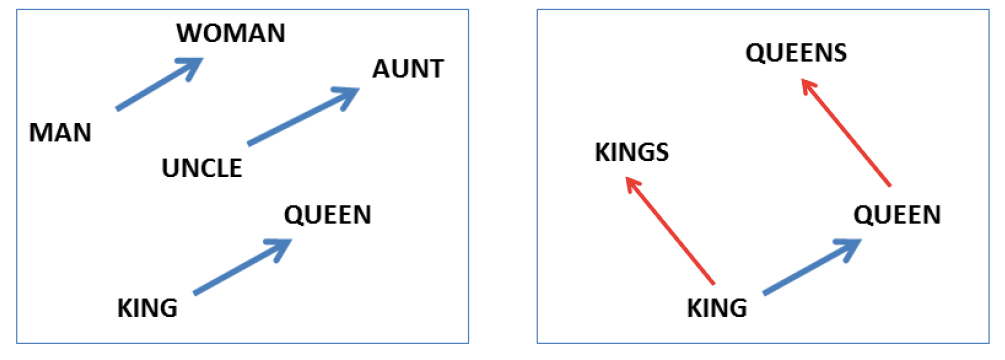
\includegraphics[width=14cm]{Images/word2vec.png}
	\centering
	\caption{Linguistic regularities preserved by the word2vec algorithm \cite{word2vec,mikolovDistirbutedRepresentationsOfWords}.}
	\label{fig:word2vec}	
\end{figure}

A similar algorithm for learning vectors is \emph{GloVe} (Global Vectors for Word Representation) \cite{glove}. GloVe is essentially a log-bilinear model with a weighted least-squares objective. The main intuition underlying the model is the simple observation that ratios of word-word co-occurrence probabilities have the potential for encoding some form of meaning.
The authors of \cite{linkingGloveWithWord2Vec} shows that GloVe and Skip-Gram model of word2vec, one explicitly factorizing a co-occurrence matrix and one implicitly factorizing a shifted-PMI matrix, are actually sharing similar objectives, though not completely the same.

It is important to note that the word-embedding techniques are using the fact that the order of words in text is important. This is not applicable for the non-target attributes within the datasets as the order is not important. We could easily permutate all the attributes and still argue that the information required to learn the features is still the same. In comparison, the order of words usually matters in the texts written by humans -- which is one of the reasons why the vector embeddings show such nice results.

The key factor in the performance of word2vec and similar methods is the size of the corpus. Common choice is up to one billion of words \cite{word2vec}.


There has also been ongoing research to use the vector embeddings on different domains than just natural languages. For example, \emph{protein-vectors} (ProtVec)~\cite{protvec} uses word2vec ideas.
The paper uses  Skip gram neural network to build a dense distributed representation for biological sequences. The method was evaluated by classifying protein sequences obtained from \emph{Swiss-Prot} \cite{uniprot} and outperformed existing classification methods. Furthermore, the method is applicable to other bioinformatics problem such as protein visualization, structure prediction, domain extraction, and interaction prediction.

\subsection{Kernels}
\label{section:kernels}
The kernel approach tackles the problem by looking at the similarities between objects. In general, kernel \cite{kernels} is a function taking two objects and returning a measurement:

\begin{definition}
	Let $\Omega$ be a set. Then \emph{kernel} K is a real-valued function of two variables from $\Omega$, i.e., 
	\begin{equation}
	\Omega \times \Omega \rightarrow \mathbb{R}
	\end{equation}
\end{definition}

To get a similarity, only the so called dot-product kernels are usually considered:
\begin{definition}
	Let $\Omega$ be a set. Then \emph{dot-product kernel} K is a real-valued function of two variables from $\Omega$ satisfying
	\begin{equation}
	K(x,y) = \langle\phi(x), \phi(y)\rangle_{\mathbb{V}},
	\end{equation}
	where $\phi$ is a \emph{feature map} $X \rightarrow \mathbb{V}$ and $\langle\cdot,\cdot\rangle_{\mathbb{V}}$ is an inner product on $\mathbb{V}$.
\end{definition}

If $\Omega$ is a space of real vectors, the dot product is a commonly considered inner product, and we can easily get so called linear kernel just by using the dot product:
\begin{equation}
K(x,y) = x^ty, \forall x,y \in \mathbb{R}^n.
\end{equation}
It is possible to use $\phi$ for rescaling and increase of dimensions. For instance, the polynomial kernel defined as 
\begin{equation}
K(x,y) = (x^ty+b)^n, x,y \in \mathbb{R}^n, r > 0, n \in \mathbb{N}, n > 0.
\end{equation}
computes the product in $\binom {d+2}2$-dimensional feature space where $d$ is a dimension of input vectors and $b$ is a parameter describing the influence of higher order terms versus lower order terms. For example, for $n=2$ the product is given by the (implicitly defined) mapping 
\begin{align*}
&\phi(\langle x_1,\dots,x_n\rangle)= \\
&\langle x_1^2,\dots, x_1^n,\sqrt{2}x_1x_2,\sqrt{2}x_1,x_3,\dots, \sqrt{2}x_{n-1}x_n,\sqrt{2b}x_1,\dots,\sqrt{2b}x_n,c\rangle.
\end{align*}

Other popular kernel is the so called \emph{radial basis function} (RBF) kernel:
\begin{equation*}
	K(x,y)=e^{-\gamma||x-y||^2},
\end{equation*}
where $\gamma$ is a parameter of the kernel.

What makes the kernel approach particularly interesting is that $\Omega$ can be an arbitrary set, not just real numbers. If we can define a mapping $\Omega$ to some space with inner product, we can  have a kernel even for objects with variable structure.

For instance, strings over some alphabet have variable structure as they can be of arbitrary length.
One of the kernels defined over strings is string subsequence kernel \cite{stringSubsequenceKernel}, which defined the similarity of two strings by the number of their common subsequences (not-necessarily contiguous):

\begin{definition}
	Let $\mathbb{A}$ be an alphabet and $x,y \in \mathbb{A}$. The \emph{string subsequence} kernel is defined as:
	\begin{equation*}
	K(x,y)=\sum_{u \in \mathbb{A}^n}\sum_{i: u = x[i]}\sum_{j: u = y[i]} \lambda ^{l(i)+l(j)},
	\end{equation*}
	where $\mathbb{A}^n$ is the set of all strings of length $n$, $s[i]$ is a subsequence of $s$ given by some set of indices $i$, $\lambda$ is a decay factor and $l(i)$ denote the total length of $s[i]$ in $s$ -- the biggest index in $i$ minus the smallest index in $i$ plus one.
\end{definition}
While this computation appears very expensive, recursive computation can be reduced to $\mathcal{O}(n|x||y|)$ \cite{stringSubsequenceKernel}. 

Another example of the string kernel is a spectrum kernel \cite{spectrumKernel}, which bases the similarity on common substrings of some predefined length.
\begin{definition}
	Given a number $k \ge 1$, the \emph{k-spectrum} of an input sequence is the set of all the k-length (contiguous) subsequences that it contains.
\end{definition}
We defined a kernel with a feature map indexed by all possible subsequences $a$ of length $k$ from alphabet $\mathbb{A}$.
\begin{definition}
	\emph{$K$}-spectrum kernel is defined as:
	\begin{equation*}
	K(x,y) = \langle (\phi_a(x))_{a \in \mathbb{A}^k}, \phi_a(y))_{a \in \mathbb{A}^k} \rangle,
	\end{equation*}
	where $\phi_a(x)$ denotes number of times $a$ occurs in $x$.
\end{definition}
A very efficient method for computing spectral kernel is to build a suffix tree for the collection of $k$-length subsequences of $x$ and $y$, obtained by moving a $k$-length sliding window across each of $x$ and $y$. At each depth-$k$ leaf node of the suffix tree, store two counts, one representing the number of times a $k$-length subsequence of $x$ ends at the leaf, the other representing a similar count for $y$. Note that this suffix tree has $\mathcal{O}(kn)$ nodes. Using a linear time construction algorithm for the suffix tree \cite{onlineConstructionOfSuffixTrees}, we can build and annotate the suffix tree in  $\mathcal{O}(kn)$ time. Now we calculate the kernel value by traversing the suffix tree and computing the sum of the products of the counts stored at the depth-$k$ nodes. The overall cost is thus $\mathcal{O}(kn)$. 

We would like to mention another string kernel called local alignment as it directly influenced our work.
\begin{definition}
	An \emph{alignment} (with gaps) $\pi$ of $p \ge 0$ positions between two sequences $x,y$ is a pair of $p$-tuples:
	\begin{equation*}
	\pi = ((\pi_1(1),\dots,\pi_1(p),\pi_2(1),\dots,\pi_2(p)) \in \mathbb{N}^{2p}
	\end{equation*}	
	that satisfies
		\begin{equation*}
		1 \le \pi_1(1) < \pi_1(2) < \dots \pi_1(n) \le |x|
		\end{equation*}
		\begin{equation*}
		1 \le \pi_2(1) < \pi_2(2) < \dots \pi_2(n) \le |y|
		\end{equation*}
\end{definition}
We can score the alignments as follows:
\begin{definition}
The \emph{local alignment} score of an alignment $\pi$ is equal to
\begin{equation*}
s_{S,g}(\pi) = \sum_{i=1}^{|\pi|}S(x_{\pi_1(i)},y_{\pi_2(i)}) - \sum_{i=1}^{|\pi|-1}
[g(\pi_1(i+1)-\pi_1(i))+g(\pi_2(i+1)-\pi_2(i))],
\end{equation*}
where S is a substitution matrix encoding score for aligning letters with other letters and $g$ is a gap penalty function.
\end{definition}
The \emph{Smith-Waterman} (SW) score is a local alignment score of the best alignment:
\begin{equation*}
SW_{S,g} = \max_{\pi \in \Pi(x,y)}s_{S,g}(\pi).
\end{equation*}
The SW score can be calculated in $\mathcal{O}(|x||y|)$ by dynamic programming with Smith-Waterman algorithm \cite{smithWaterman}.
\begin{equation}
SW(i,j)= \max
	\begin{cases}
	0, \\
	SW(i-1,j)+S(x_i, y_j), \\
	\max_k{SW(i-k,j)-g(k)}, \\
	\max_l{SW(i,j-l)-g(l)}. \\
	\end{cases}
\end{equation}
$SW(i,j)$ stands for the similarity of two segments ending in $x_i$ and $y_j$ respectively.

Unfortunately, SW score does not have to be a valid inner-product kernel~\cite{smithWatermanKernel}. However, a convolution kernel can be defined as follows:
\begin{equation}
K_{LA}^{(\beta)}(x,y) = \sum_{\pi \in \Pi(x,y)}e^{\beta s_{S,g(\pi)}},
\end{equation}
where $\beta$ is a parameter. It can be shown that the SW score is approached by the limit:
\begin{equation}
\lim_{\beta \rightarrow \infty} \frac{1}{\beta}\ln(K_{LA}^{(\beta)}(x,y)) = SW(x,y).
\end{equation}
 Furthermore, it can be shown that if there is no gap penalty a SW score is a kernel \cite{swNoGapKernel}.

Another domains where kernels were applied is the space of graphs \cite{graphKernels} and images \cite{imageKernels}. Again, we cannot apply string or graph kernels directly to the dataset space as the order of character or vertices matters. 

Having an inner product kernel has many advantages. Computation of the inner product kernel can be carried out without explicitly using the $\phi$ function and computing the inner product. Mapping to the feature space can be very expensive or not feasible at all. For example, the RBF kernel with $\gamma = 1$ is actually computing the inner product in an infinite dimensional feature space:
\begin{equation*}
e^{-||x-y||^2} = \sum_{j=0}^{\infty}\frac{(x^Ty)^j}{j!}e^{(-\frac{1}{2}||x||^2)}e^{(-\frac{1}{2}||y||^2)}.
\end{equation*}
Such computation of inner product in the feature space using only values in the input space is sometimes being referred to as a \emph{kernel trick}.

Many methods benefit from the kernel trick or can be extended to do so. For example, \emph{support vector machine} (SVM) \cite{svm} can use the kernel to separate non-linearly separable sets by performing the separability in the feature space instead. The ability of kernels to be used in such a way is demonstrated in Figure \ref{fig:nonlinearitythroughkernels} by using the scikit-learn library \cite{scikit-learn}. First, two categories of points are generated -- blue points distributed over the circle with some small noise and red circles distributed around the circle with bigger radius. Clearly, the blue set is not linearly separable from the red set. Using another method enhanceable by the kernel trick -- \emph{kernelized PCA} with the RBF kernel \cite{kernelizedSVM} -- we can achieve the linear separability.

\begin{figure}
	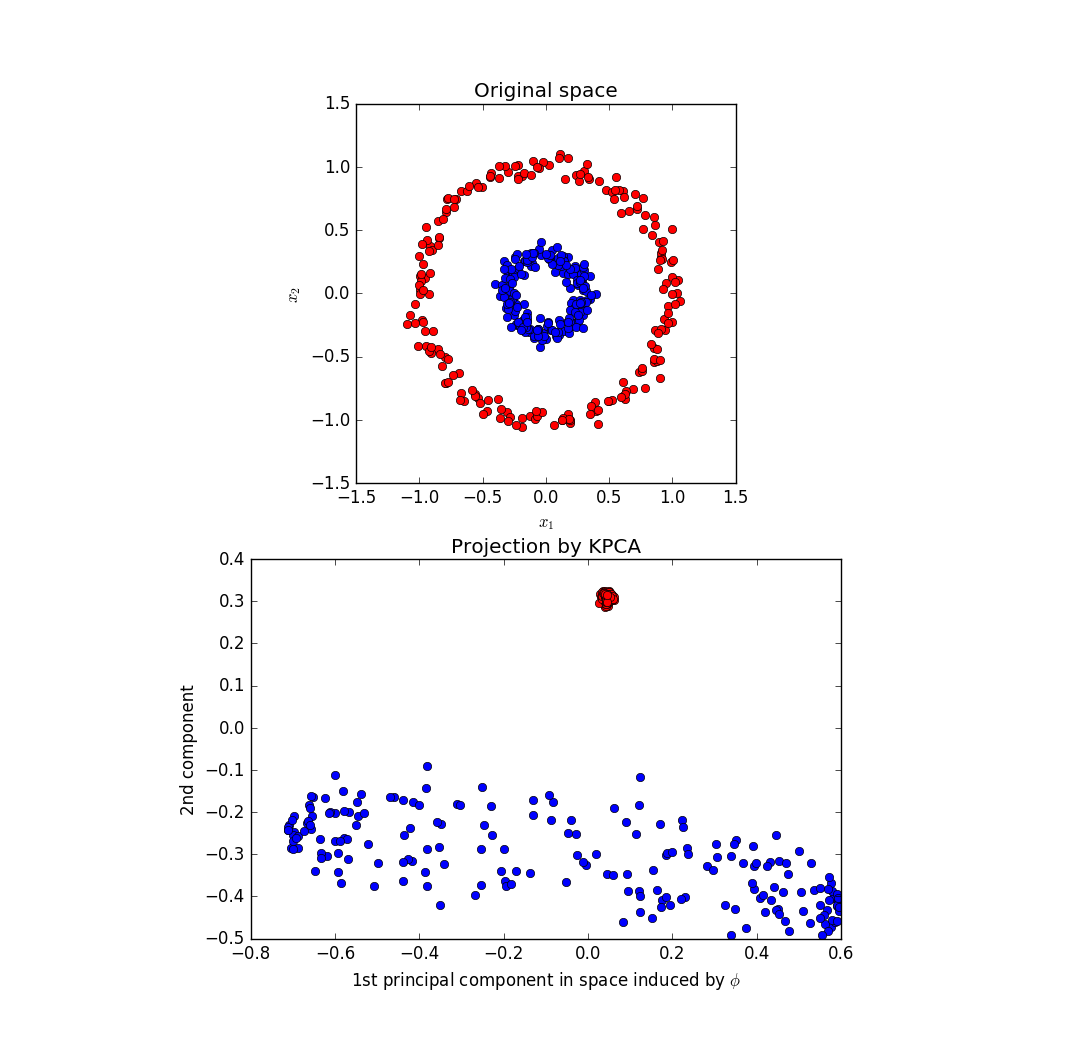
\includegraphics[width=16cm]{Images/nonlinearitythroughkernels.png}
	\centering
	\caption{Example of using the kernelized PCA in the scikit-learn library \cite{scikit-learn} to make the data linearly separable.}
	\label{fig:nonlinearitythroughkernels}	
\end{figure}
The kernelized PCA opens many options as it can map arbitrary space with kernel to the vector of the desired length. Reducing the dimensions to two or three is especially useful as it can be visualized easily.

Metalearning is also used to aid the methods with kernels as choosing a right kernel can be crucial to solve the problem at hand. Authors of \cite{kernelSelectionMetalearning} use meta-learning to select the right kernel for SVM by measuring the problem characteristics using classical, distance and distribution-based statistical information. In \cite{kernelLearningByTransferLearning} the kernel is automatically selected based on knowledge transferred from the results on related data.

\section{Non-propositional Approach to Metalearning}
\label{section:NonpropositionalApproachToMetalearning}

All of the methods for algorithm selection problem discussed so far used the propositional approach -- every dataset was represented by the metadata vector of fixed size. However, the problem is highly non-propositional as the number of attributes varies throughout the datasets. According to the authors of \cite{BrazdilMetalearning-2009}, the most common approach to deal with this problem is to do some form of aggregation, for example use mean skewness as an aggregation of every attribute with skewness. It is expected that important information will be lost in the process. In \cite{jaOndraMetadataMetric}, we partially addressed the problem by adding the special attribute metadata. First, we identified the most significant attributes. The significance of attribute was identified by the \emph{joint entropy} of a target class and attribute:
\begin{equation}
H(A,C) = - \sum_{v \in Val(A)}\frac{n(A(v))}{n}
\sum_{t \in Val(C)}\frac{n_t(A(v))}{n(A(v))}\log_2\frac{n_t(A(v))}{n(A(v))},
\end{equation}
where $n$ is the number of observations, $n(A(v))$ is the number of observation with the value $v$ of the attribute and $n_t(A(v))$ is the number of observations with the value $v$ of the attribute and with the value $t$ of the target attribute.
For the continuous attributes (for them the direct entropy computation is not desirable) the discretization of the values was used instead. We then chose a number $k$ and the attribute metadata of $k$ most significant attributes were added to the propositional representation of the datasets. We specifically used entropy (see Equation \ref{equation:entropy}) of the $i$-th most significant attribute.
It is however easy to extend the approach with the arbitrary attribute metadata.

Alternatively, in \cite{KalousisDesignImplementationAndPerfromance} two measures of association are used, one for continuous attributes and one for discrete ones. For continuous attributes, the absolute value of the correlation coefficient is used, for discrete attributes, the \textit{Goodman and Kruskal's tau} \cite{AgrestiCategoricalDataAnalysis} coefficient also known as the concentration coefficient is used. The problem of the various number of attributes is dealt with by introducing a histogram of these attributes with the fixed number of bins.

Both the approaches above are merely pushing the problem further. As we have chosen fixed number of most significant attributes or bins, what happens if we have to deal with datasets with billion times more attributes than the number of bins?

Kalousis et al. \cite{RepresentationalIssuesInMetalearning} solve the problem of varying attributes by defining a distance measure on the attribute space. The dataset distance is then similar to the distances used in clustering -- either \emph{Single Linkage Based Similarity} (similarity taken is the maximum similarity between the attributes) or \emph{Average Linkage Based Similarity} is used. Attribute similarity is calculated as 1 minus the Manhattan distance defined on the attribute metadata. This can handle the non-propositional approach and the authors demonstrated that such distance function is useful in metalearning. However, we can still imagine datasets that are very different but whose Single Linkage Based Similarity is high (one common attribute, many very different attributes) and similar datasets whose Average Linkage Based Similarity is low (many similar attributes but distant from others).
A possible explanation is that the Single Linkage Based Distance  does not necessarily produce a metric:
\begin{observation}
	Given arbitrary metric $\attributeDistance$ on the attribute space whose cardinality is at least two there exist datasets $a,b,c$ such that the distance between datasets $\globalDistance$ induced by Single Linkage Clustering 
	$$\globalDistance(a,b)=\min_{i, e_i \in a, j, e_j \in b}(\attributeDistance(e_i,e_j))$$ is not a metric on the dataset space.
	\begin{proof}
	The attribute space has at least two distinct elements, we will call them $e_1, e_2$. Let $a=\{e_1\}$, $b=\{e_2\}$ and $c=\{e_1, e_2\}$. Then $$\globalDistance(a,c)+\globalDistance(b,c) = 0+0 < \globalDistance(a,b),$$
	which breaks the triangle inequality.
	\end{proof}	
\end{observation}

We can also find the similar counterexample for the Average Linkage Based Distance:
\begin{observation}
	Given arbitrary metric $\attributeDistance$ on the attribute space whose cardinality is at least two there exist datasets $a,b$ such that the distance between datasets $\globalDistance$ induced by the Average Linkage Clustering $$\globalDistance(a,b)=\frac{1}{|a||b|}\sum_{i, e_i \in a}\sum_{j, e_j \in b}\attributeDistance(e_i,e_j))$$ is not a metric on the dataset space.
	\begin{proof}
		The attribute space has at least two distinct elements, we will call them $e_1, e_2$. Let $a=b=\{e_1, e_2\}$. Then $$\attributeDistance(a,b)=\frac{1}{4}(0+\attributeDistance(e_1, e_2)+0+\attributeDistance(e_,e_1))=\frac{1}{2}\attributeDistance(e_1,e_2)>0,$$
		which breaks the coincidence axiom.
	\end{proof}	
\end{observation}

\section{Distance Using Attributes}
\label{section:distanceUsingAttributes}
As discussed in the beginning of this chapter, ability to process unstructured data can significantly improve the tasks defined on those data as we can use bigger palette of approaches. Unfortunately, the methods proposed on the strings and graph spaces are not out of the box applicable to the space of datasets but rather can serve as an inspiration. For example, the Smith-Waterman algorithm looks interesting, but it was designed with the fact that the order of letter matters in mind. With the datasets, it should not matter if we permutate the attribute. The target function should be learnable all the same as we can preprocess the attributes by inverse permutation. The non-propositional approaches reviewed in the previous section are either losing information or lacking properties usually important for the distance functions.

Authors of \cite{DistancesAndIndefiniteKernelsForTheSetsOfObjects} review possible ways of using the distance measures defined on $\mathbb{X}$ in
order to define distance measures on the power set $2^\mathbb{X}$ of $\mathbb{X}.$
The most promising is the distance measure defined as follows:
\begin{equation}
D_M(A,B) = \min_{R_i \in R}{(\sum_{(a_k, b_j) \in R_i}{\attributeDistance(a_k, b_j)}+(|B \setminus R_i(A)|+|A \setminus R_i^{-1}(B)|)\frac{M}{2})},
\end{equation}
where $\attributeDistance$ is a distance between elements of some space $\mathbb{S}$, $A,B \subseteq \mathbb{S}$, $R_i$ is a matching (each element at most once) on $A \times B$, and $M$ is a maximum distance of $\attributeDistance$ on $\mathbb{S}$. $D_M$ can be also viewed as a distance that finds optimal mapping between elements of $A,B$ and can decide to omit some elements by getting $\frac{M}{2}$ penalty.
Authors of  \cite{polynomialTimeComputableMetricBetweenPointSets} prove that the $D_M$ is a metric if $\attributeDistance$ is a metric. Furthermore, $D_M$ is computable in the polynomial time.
We can treat datasets as composed by attributes and use $D_M$ by defining a distance $\attributeDistance$ on attribute space. However, there are still reasons that render this approach impractical for metalearning.
The distance measure $D_M$ requires $M$. The computation of $M$ may not be feasible or not known in advance, especially if the attribute distance was not normalized. Additionally, some attributes may be more significant than the others. Not matching some insignificant attributes because of fewer attributes in the second dataset (for example with low entropy for predicting the target attribute) will still result in $\frac{M}{2}$ distance. Also, algorithm can decide not to match some attributes with high difference and get only $\frac{M}{2}$ penalty. For example, when comparing two datasets with single attributes, the results will be the same if the attributes are really distant ($M$) or somewhat distant ($\frac{M}{2}$). In both cases the $D_M$ will return $\frac{M}{2}$.

In this section, we propose several approaches that can handle the non-propositional dataset representations without any trade-offs. We have already published their descriptions and experiments validating their asset in ~\cite{diplomka,jaIcannga2013,SSCI2014,jaCEC2015,jaSSCI2015}. Each one is based on the idea of attribute aligning where the order of attributes is not important. By supplying a function measuring the distance between individual attributes (like in \cite{RepresentationalIssuesInMetalearning}), we could try to align the attributes in the way that minimizes the sum of distances between aligned attributes. To avoid confusion, we will always denote attribute distance measure as $\attributeDistance$. The name was not chosen randomly. The upper case $\globalDistance$ -- as always -- will denote the final dataset distance measure. As we will see, we will piece $\globalDistance$ out of smaller $\attributeDistance$s, hence the name.

Although we are aiming to handle the non-propositional approach, we will start with propositional situation to describe the approach, and extend it later to handle varying amount of attributes.
For now let us suppose that there is the same number of attributes in every dataset (and hence the same number of attribute metafeatures).

\begin{definition}
Given a distance function between attributes $\attributeDistance$, two datasets $a,b$ and a bijection $f$ between the attributes of $a,b$ we define the dataset distance induced by the bijection between the datasets as:
\begin{equation}
\globalDistance_f(a,b)=\sum_{k=1}^{n}{(\attributeDistance(a_k,f(a_k)))},
\label{eq:attdist}
\end{equation}
where $a_k$ is the $k$-th attribute of $a$ and $f(a_k)$ corresponding attribute in dataset b given by the bijection $f$.
We will sometimes refer to the $\globalDistance_f$ as the \emph{cost} of $f$.
\end{definition}
We would like to match the attributes as best as possible to get the lowest possible distance $\globalDistance_f$, so optimally we are looking for $f^*$:
\begin{equation}
f^*= \mathrm{argmin}_f(\globalDistance_f).
\label{eq:argmin}
\end{equation}
We will denote $f^*$ as an optimal alignment.

From this, the general distance between datasets can be derived:
\begin{equation}
\globalDistance(a,b) = \globalDistance_{f^*}(a,b).
\end{equation}

Now suppose that the number of attributes is different. We transform this case to the previous one by adding dummy attributes into the dataset with less attributes. We can think of a dummy attribute in a similar way as of a gap penalty in the Smith-Waterman algorithm. There are two approaches how to do this. Suppose $\mathbb{A}$ is a space of attributes. Either $dummy \in \mathbb{A}$ or $dummy \notin \mathbb{A}$. In the former case, nothing is needed, as the distance function between attributes is already defined if the $\dummy$ attribute is on the input. In the latter case, it is needed to extend the distance function by defining the distance between a regular attribute and the $\dummy$ one.
In the further text, we will refer to the attribute space with the $\dummy$ attribute as to the \emph{extended attribute space}. If it is clear from the context, we will sometimes refer to extended attribute space simply as attribute space. $Dummy$ attribute will be referred to as $\dummy$ or specifically to $\dummyinside$ if the dummy attribute is already in the attribute space and $\dummyoutside$ if the attribute is newly created.
We will discuss the pros and cons of these approaches as well as how to choose the right attribute for the $\dummy$ one, and how to define the distance between a regular attribute and a $\dummy$ one respectively in Section \ref{section:theoreticalProperties}.

From now on, we can suppose that if we are aligning two datasets that they have the same number of attributes, and that one dataset was to some extent enriched with some number of $\dummy$ attributes, so the amount of attributes matches.

There are $n!$ bijections from $a$ to $b$. It is costly to enumerate them, so it is desired to eliminate some of the bijections in advance. In this work, we came up with two approaches that vary in the generality of the attribute distance and computational complexity.
\begin{definition}
\emph{Evaluation function} $\sigma$ is a function mapping attributes to $\mathbb{R}$.
\end{definition}

In our first approach, we suppose we have $\sigma$ (for example, number of distinct values), and the attribute distance is defined as follows:
\begin{equation}
\attributeDistance(a_k, f(a_k))=|\sigma(a_k)-\sigma(f(a_k))|.
\label{eq:sigma}
\end{equation}

\begin{theorem}
Given datasets $a,b$ and a bijection $f$, if we sort $a$ and $b$ by $\sigma$ in the ascending order obtaining $a',b'$ we can find $f'$ such that
\begin{equation}
\globalDistance_{f'}(a',b')=\globalDistance_f(a,b).
\label{eq:df}
\end{equation}
\end{theorem}
\begin{proof}
Let $\pi _{a}$, $\pi _{b}$ be the permutations used to sort $a,b$. Define $f'$ as follows:
\begin{equation}
f'(a'_i)=\pi _{b}(f(\pi _{a}^{-1}(a'_i))).
\label{eq:fai}
\end{equation}
We have to prove that for every $k$ there is $j$ such that $|\sigma(a_k)-\sigma(f(a_k))|=|\sigma(a'_j)-\sigma(f'(a'_j))|$. As a candidate for $j$ we take such $j$ that $a'_j=\pi_{a}(a_k).$ Such $j$ exists and it is unique as $\pi_{a}$ is a permutation. Observe that sorting permutation does not affect $\sigma.$ Therefore $\sigma(a'_j)=\sigma(\pi_{a}(a_k))=\sigma(a_k).$ %Mark index of $f(a_k)$ as $z$. 
Directly from the observation the following equation can be derived: 
\begin{equation}
\sigma(f'(a'_j))=\sigma(\pi _{b}(f(\pi _{a}^{-1}(a'_j))))= \sigma(f(\pi _{a}^{-1}(a'_j)))=\sigma(f(a_k)),
\label{eq:faj}
\end{equation}
which concludes the proof as the $j$ is unique and it always exists.
\end{proof}

\begin{corollary}
We can exclusively use this canonical representation and without the loss of generality, suppose that $a,b$ are sorted by $\sigma$.
\end{corollary}

\begin{definition}
We say that the bijection $f$ is the \emph{identity alignment} if $\forall i,a_i \in a:f(a_i)=b_i$. 
\end{definition}
The example of the identity alignment is shown in Figure~\ref{fig:identity}.
\begin{figure}
	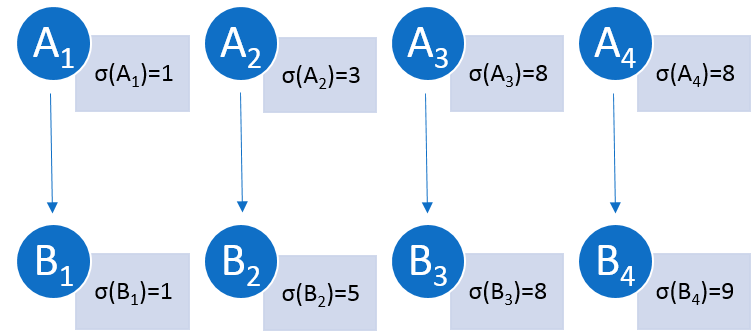
\includegraphics[width=9.5cm]{Images/identity.png}
		\centering
	\caption{Example of the identity alignment. If the attributes are sorted by $\sigma$, each attribute is aligned to the attribute with the same order.}
	\label{fig:identity}	
\end{figure}

\begin{theorem}
\label{mainproof}
Identity alignment is optimal.
\end{theorem}
\begin{proof}
Given the bijection $f$ that is not an identity alignment and is optimal, we will show that it can be either transformed to identity alignment or it is not optimal, which leads to a contradiction. Find the lowest $i$ such that $f(a_i)\neq b_i $. Such $i$ exists, because $f$ is not an identity alignment. We mark the index of attribute $f(a_i)$ as $z$. Because $f$ is a bijection, we can find $j$ such that $f^{-1}(b_i)=a_j$. Take a bijection $f'$ that is the same as $f$ with the exception of arguments $i$ and $z$:
 \begin{eqnarray}
    f'(a_i)&=b_i, \nonumber \\
    f'(a_j)&=b_z.
    \end{eqnarray}
In other words, $f'$ is more similar to identity alignment than $f$. The whole transformation is shown in Figure~\ref{fig:transformation}. 
\begin{figure}	
		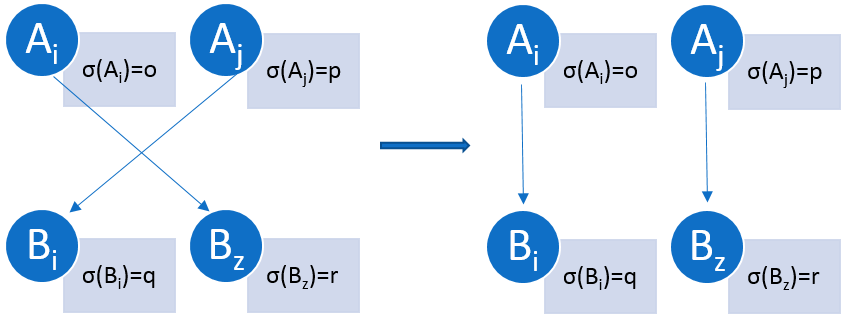
\includegraphics[width=9.5cm]{Images/transformation.png}
		\centering
	\caption{Example of transformation. Find attributes that falsify identity alignment and switch them. At least one less pair of attributes now falsifies the identity alignment.}	
	\label{fig:transformation}	
\end{figure} 

We have to verify that:
 \begin{align}
    d_f &\geq d_{f'}. \\
    \sum_{k=1}^{n}{(|\sigma(a_k)-\sigma(f(a_k))|)}     &\geq \sum_{k=1}^{n}{(|\sigma(a_k)-\sigma(f'(a_k))|)}.
    \end{align}
    
The $d_f$ and $d_f'$ differs only in positions $i$ and $j$. Thus we can simplify the equation to:
\begin{align}
    \sum_{k \in {i,j}}{(|\sigma(a_k)-\sigma(f(a_k))|)} 
    &\geq \sum_{k \in {i,j}}{(|\sigma(a_k)-\sigma(f'(a_k))|)}.  
\end{align}    
\begin{align}    
    &|\sigma(a_i)-\sigma(b_z)|+|\sigma(a_j)-\sigma(b_i)| \geq |\sigma(a_i)-\sigma(b_i)|+|\sigma(a_j)-\sigma(b_z)|. 
\end{align} 
If we denote values $\sigma(a_i),\sigma(a_j),\sigma(b_i),\sigma(b_z)$ as $o,p,q,r$, we can simplify the equation further:
\begin{equation}
|o-r|+|p-q|\geq |o-q|+|p-r|.
\label{eq:targetCondition}
\end{equation}
Because we use sorted canonical representation and because of the fact we have taken the lowest $i$ possible we know that:
\begin{equation}
o\leq p,
\label{eq:op}
\end{equation}
\begin{equation}
q \leq r.
\label{eq:qr}
\end{equation}
There are 6 possible orderings of $o,p,q,r$ that fulfils these two equations. The enumeration of these 6 cases is in Table \ref{table:caseEnum}.

\begin{table}[htbp]
\caption{Equation \ref{eq:targetCondition} holds for every possible case.}
\label{table:caseEnum}
\centering
\begin{tabular}{ |c | c | c |c | }
  \hline
  ORDER & $|r-o|+|q-p|$ & $|q-o|+|r-p|$ & $\geq$ \\
  \hline                       
  opqr & $|q-r|+2*|q-p|+|p-o|$ & $|q-r|+2*|q-p|+|p-o|$ & $=$ \\
  oqpr & $|r-p|+2*|q-p|+|q-o|$ & $|q-o|+|r-p|$ & $\geq$\\
 oqrp & $2*|q-r|+|q-o|+|r-p|$ & $|q-o|+|r-p|$ & $\geq$\\
  qopr & $|r-p|+|q-o|+2*|p-o|$ & $|q-o|+|r-p|$ & $\geq$\\
  qorp & $2*|r-o|+|q-o|+|r-p|$ & $|q-o|+|r-p|$ & $\geq$\\
  qrop & $2*|r-o|+|q-r|+|p-o|$ & $2*|r-o|+|q-r|+|p-o|$ & $=$\\
  \hline  
\end{tabular}
\end{table}
In every presented case, the $f'$ is at least as good as $f$, and the position $i$ no longer falsifies the identity alignment. If $f'$ is still not the identity alignment, we can repeat the previous step until we get an identity alignment because the number of attributes is finite.
\end{proof}

\begin{corollary}
Based on Theorem \ref{mainproof}, a more efficient algorithm for the attribute alignment can be derived with the complexity of alignment equal to $\mathcal{O}(n\log(n))$, where $n$ is the number of attributes.
\end{corollary}

%http://get-software.net/macros/latex/contrib/algorithm2e/doc/algorithm2e.pdf
\IncMargin{1em}
\begin{algorithm}
\SetKwInOut{Input}{input}\SetKwInOut{Output}{output}
\tcp{Pseudocode for an attribute alignment algorithm with constrained attribute distance function running in $\mathcal{O}(n\log(n))$.}
\Input{a $\leftarrow$ List of attributes}
\Input{b $\leftarrow$ List of attributes}
\Input{$\sigma \leftarrow$ Attribute evaluation function: $\mathbb{A}\rightarrow \mathbb{R}$}
\Output{Distance between a and b}
\BlankLine
Add dummy attributes into the list with less attributes\;
Sort both list of attributes by $\sigma$\;
totalDistance $\leftarrow 0$\;
\For{$i\leftarrow 0$ \KwTo $i < \text{len}(a)$}{
totalDistance $\leftarrow$ $|\sigma(a[i])-\sigma(b[i])|$\;
}
\Return totalDistance\;
\caption{Attribute alignment}
\label{algo:attributeAlignmentMasterThesis}
\end{algorithm}\DecMargin{1em}

The pseudocode is outlined in Algorithm \ref{algo:attributeAlignmentMasterThesis}.

From the algorithm, the total computational complexity can be inferred. The sorting can be done in $\mathcal{O}(n\log(n))$, where $n$ is the number of attributes. The enumeration can be done in $\mathcal{O}(n)$, the evaluation of $\sigma$ for every attribute takes $\mathcal{O}(nc(\sigma))$~steps, where $c(\sigma)$ is a cost of calling the evaluation function for a single attribute. Therefore, the total complexity of Algorithm \ref{algo:attributeAlignmentMasterThesis} is  $\mathcal{O}(n(\log(n)+c(\sigma))).$

In our second approach, we allow arbitrary function $\attributeDistance$ measuring the distance between two attributes. Given two datasets $a,b$ and attribute distance function $\attributeDistance$, a distance matrix $M$ can be easily built up:
\begin{equation}
M_{i,j} = \attributeDistance(a_i,b_j).	
\end{equation}
We can see the distance matrix $M$ as the cost function and the aligning of attributes as an assignment, which leads to an assignment problem. The assignment problem is well known. The polynomial algorithm -- in the graph theory known as the Hungarian algorithm -- solving the assignment problem in $\mathcal{O}(n^4)$ was described in \cite{KuhnHungarian}. The $\mathcal{O}(n^3)$ implementation of the Hungarian algorithm was later published in \cite{KarpHungarian}.
Before the algorithm itself we will state few definitions needed. Given a graph $G = (V, E)$:  

\begin{definition}
A \emph{matching} is a subset $M \subseteq E$ such that $\forall v \in V$ at most one edge in $M$ is incident upon V.
\end{definition}

\begin{definition}
A \emph{perfect matching} is an $M$ in which every vertex is adjacent to some edge in $M$.
\end{definition}

\begin{definition}
A vertex \emph{labelling} is a function $l:V\mapsto R.$
\end{definition}

\begin{definition}
Vertex $v$ is \emph{matched} if it is an endpoint of edge in $M$, otherwise it is \emph{free}.
\end{definition}

\begin{definition}
The \emph{equality graph} with the respect to the labelling l is $G=(V,E_l)$, where $E_l=\{(x,y)|x,y \in V, l(x)+l(y)=w(x,y)\}.$
\end{definition}

\begin{definition}
A path is \emph{alternating} if its edges alternate between $M$ and $E \setminus M$.
\end{definition}

\begin{definition}
An alternating path is \emph{augmenting} if both endpoints are free.
\end{definition}

\begin{definition}
Define \emph{neighbour} of $u \in V$ and set $S\subseteq V$ to be:
\begin{equation}
N_l(u)={v:(u,v)\in E_l}, N_l(S)=\cup_{u\in S}N_l(u).
\label{eq:nlu}
\end{equation}
\end{definition}
%\pagebreak
Given the definitions above, the pseudocode for the Hungarian algorithm can be outlined, as per Algorithm \ref{algo:hungarianAlgorithm}.

\IncMargin{1em}
\begin{algorithm}
\SetKwInOut{Input}{input}
\SetKwInOut{Output}{output}
\tcp{Pseudocode of the Hungarian Algorithm solving assignment problem in $\mathcal{O}(n^3)$.}
\Input{$(X \cup Y,E)$ $\leftarrow$ Weighted bipartite graph }
\Output{Minimal assignment}
\BlankLine
Generate initial labelling $l$ and matching $M$ in $E_l.$ \;
\While{\upshape $M$ is not perfect}{
	$u \leftarrow$  pick free vertex $\in X$\;
	$S \leftarrow$  $\left\{u\right\}$\;
	$T \leftarrow$  $\left\{\right\}$\;
	\If{$N_l(S)=T$}{
	update labels (forcing $N_l(S)\neq T$) \;
	$a_l \leftarrow \min_{s \in S,y\notin T}(l(x)+l(y)-w(x,y)) $\;
	$
	 l'(v) \leftarrow
	 \begin{cases}
	 l(v)-a_l; \mbox{ if } v \in S, \\
	 l(v)+a_l; \mbox{ if } v \in T, \\
	 l(v); \mbox{ otherwise}.
	 \end{cases}
	$
	}
	\If{$N_l(S)\neq T$}{
	pick $y \in N_l(S)-T$\;
	If $y$ free, $u-y$ is augmenting path. Augment $M$ and go to 2\;
	If $y$ matched, say to $z$, extend alternating tree: \\ $S \leftarrow S\cup {z},T \leftarrow T\cup {y}$. Go to 6\;
	}
}

\Return minimalAssignment\;
\caption{Hungarian algorithm}\label{algo:hungarianAlgorithm}
\end{algorithm}\DecMargin{1em}


We can use this algorithm to find the best assignment of the attributes. From the assignment the total distance between attributes can be computed as the sum of individual distances defined by the alignment as already seen in Algorithm \ref{algo:attributeAlignmentMasterThesis}. If  $\attributeDistance$ was defined in the same manner as in the first approach, we would get the same result (Algorithm \ref{algo:attributeAlignmentMasterThesis} is a special case of Algorithm \ref{algo:attributeAlignmentHungarian}). The difference is that this version allows for an arbitrary function measuring distance between attributes as an input.

For the sake of generalization, we will define $IAttributeDistance$ interface that will represent such attribute distance. This interface is outlined in Algorithm \ref{interface:IAttributeDistance}. The total complexity of the algorithm depends on the complexity of this function and is $\mathcal{O}(n^3+n^2\sigma(n))$, where $n$ is the number of attributes and $\sigma(n)$ is the complexity of the attribute distance function. The whole algorithm that uses the Hungarian Algorithm and $IAttributeDitance$ is outlined in Algorithm \ref{algo:attributeAlignmentHungarian}.

\IncMargin{1em}
\begin{algorithm}
	\SetKwInOut{Input}{input}
	\SetKwInOut{Output}{output}
	\tcp{Interface for measuring distance between two attributes.}
	\Input{$a \leftarrow$ First attribute}
	\Input{$b \leftarrow$ Second attribute}
	\Output{ $d \in \mathbb{R}, d$ is an attribute distance $\attributeDistance$ between $a, b$. }
	\BlankLine
	\caption{$IAttributeDistance$: Dataset distance interface}
	\label{interface:IAttributeDistance}
\end{algorithm}\DecMargin{1em}

\IncMargin{1em}
\begin{algorithm}
\SetKwInOut{Input}{input}\SetKwInOut{Output}{output}
\tcp{Pseudocode for an attribute alignment algorithm using Hungarian Algorithm for the alignment.}
\Input{$a \leftarrow$ First list of attributes}
\Input{$b \leftarrow$ Second list of attributes}
\Input{$\attributeDistance$ $\leftarrow$ $IAttributeDistance$ Function}
\Output{Distance between $a$ and $b$}
\BlankLine
Add dummy attributes into the list with less attributes\;
$M[i,j] \leftarrow \attributeDistance(a[i], b[j])$\;
assignments $\leftarrow$ HungarianAlgorithm($M$)\;
totalDistance $\leftarrow$ 0\;
\For{\upshape $i\leftarrow 0$ \KwTo $i < \text{len}(a)$}{
totalDistance $\leftarrow M[i][\text{assignments}[i]]$\;
}
\Return totalDistance\;
\caption{Attribute assignment}\label{algo:attributeAlignmentHungarian}
\end{algorithm}\DecMargin{1em}

It is arguable whether we should come with the distance function between attributes that covers all cases including the distance between categorical and numerical attribute. We suppose that the attribute metafeatures of categorical and numerical attributes will vary, thus making it difficult to specify the distance. To solve this problem, the distance could be split into two parts: the distance between numerical attributes and the distance between categorical attributes. The final distance would be then the total of the sub-distances. To generalize this idea, we could go a step further and define selectors over the list of attributes. The selector would be a function accepting a list of attributes and returning a subset of the list. The selector interface is described in the $ISelectorInterface$ (Algorithm \ref{interface:ISelectorInterface}). Specific examples conforming to this $ISelectorInterface$ are Algorithms \ref{algo:NumericalAttributesSelector} (numerical selector) and \ref{algo:CategoricalAttributesSelector} (categorical selector). An attribute distance function could then be provided for each selector. Optionally, weights could be defined for each selector describing the importance of such selector (e.g. categorical attributes could be weighted more than numerical). This is outlined in Algorithm \ref{algo:combinedAlignmentHungarian}. To illustrate how to invoke this algorithm for the example above (sum of distances of categorical and numerical attributes), we would set the selectors to just defined ones: $$[NumericalAttributesSelector, CategoricalAttributesSelector].$$ The attribute distance between categorical attributes and numerical attributes would be needed to invoke the whole algorithm. Also, note that Algorithm \ref{algo:combinedAlignmentHungarian} is a generalization of Algorithm \ref{algo:attributeAlignmentHungarian}. To obtain the equal results we have to invoke Algorithm \ref{algo:combinedAlignmentHungarian} with the single distance, selector that filters nothing and weight $1$. This will allows us to reuse some theorems that are valid for Algorithm \ref{algo:hungarianAlgorithm}. We can also use the idea with selectors for the Attribute Alignment algorithm (Algorithm \ref{algo:attributeAlignmentMasterThesis}). We will call the modified Attribute Alignment with selectors as Combined Attribute Alignment. However, we will not explicitly provide the outline of this algorithm as it is just Algorithm \ref{algo:combinedAlignmentHungarian} with the Attribute Alignment algorithms instead of Attribute Assignment.

The last thing remaining is to make the assignments algorithms compatible with the $IDatasetDistance$. The first accepts two lists of attributes, the latter two datasets. As the transformation of dataset is trivial and more of a technicality we will treat the dataset to be implicitly convertible to the list of attributes (but not vice-versa) by just extracting all the attributes out of a dataset. This will make all assignment type algorithms compatible with $IDatasetDistance$ interface.

\IncMargin{1em}
\begin{algorithm}
	\SetKwInOut{Input}{input}
	\SetKwInOut{Output}{output}
	\tcp{Interface for selecting subset of attributes.}
	\Input{$a \leftarrow$ List of attributes}
	\Output{ $a',a' \subseteq a$ }
	\BlankLine
	\caption{$ISelectorInterface$: Interface for selecting subset of attributes.}\label{interface:ISelectorInterface}
\end{algorithm}\DecMargin{1em}

\IncMargin{1em}
\begin{algorithm}
	\SetKwInOut{Input}{input}
	\SetKwInOut{Output}{output}
	\tcp{Selector for selecting numerical attributes.}
	\Input{$a \leftarrow$ List of attributes}
	\Output{ $a',a' \subseteq a$. }
	\BlankLine
	\Return $a.\text{where}(x:x \text{ is Numerical})$\;
	\caption{$NumericalAttributesSelector$: $ISelectorInterface$ for selecting numerical attributes}\label{algo:NumericalAttributesSelector}
\end{algorithm}\DecMargin{1em}

\IncMargin{1em}
\begin{algorithm}
	\SetKwInOut{Input}{input}
	\SetKwInOut{Output}{output}
	\tcp{Selector for selecting categorical attributes.}
	\Input{$a \leftarrow$ List of attributes}
	\Output{ $a',a' \subseteq a$. }
	\BlankLine
	\Return $a.\text{where}(x:x \text{ is Categorical})$\;
	\caption{$CategoricalAttributesSelector$: $ISelectorInterface$ for selecting numerical attributes}\label{algo:CategoricalAttributesSelector}
\end{algorithm}\DecMargin{1em}

\IncMargin{1em}
\begin{algorithm}
\SetKwFunction{AttributeAssignment}{AttributeAssignment}
\SetKwInOut{Input}{input}\SetKwInOut{Output}{output}
\tcp{Pseudocode for distance measure combining multiple attribute assignments for each selectors.}
\Input{$a \leftarrow$ First list of attributes}
\Input{$b \leftarrow$ Second list of attributes}
\Input{selectors $\leftarrow$ List of selectors}
\Input{$w \leftarrow$ List of weights}
\Input{distanceMeasures $\leftarrow$ List of $IAttributeDistance$ functions}
\Output{Distance between $a$ and $b$}
\BlankLine
totalDistance $\leftarrow$ 0\;
\For{\upshape $i\leftarrow 0$ \KwTo $i < \text{len(selectors)}$}{
$a' \leftarrow$ selectors$[i](a)$\;
$b' \leftarrow$ selectors$[i](b)$\;
$\attributeDistance \leftarrow$ distanceMeasures$[i]$\;
Add dummy attributes into $a' \text{ or } b'$ - whichever has less attributes\;
totalDistance $\leftarrow w[i]*$attributeAssignment$(a', b', \attributeDistance)$\;
}
\Return totalDistance\;
\caption{Combined Attribute Assignment}
\label{algo:combinedAlignmentHungarian}
\end{algorithm}\DecMargin{1em}

\section {Examples}
In this section, we will demonstrate the use of our algorithms.
Let us start with Algorithm \ref{algo:attributeAlignmentMasterThesis}. Suppose that we have two datasets $a$ and $b$. The possible values of individual attributes are shown in Tables \ref{table:dataseta} and \ref{table:datasetb}.
\begin{table}[htbp]
\caption{Possible values of dataset $a$.}
\label{table:dataseta}
\centering
\begin{tabular}{ |c | c | c |c | }
  \hline
  $Att1$ & $Att2$ & $Att3$ \\
  \hline                       
  Blue & Small & Common \\
  White & Medium & Rare \\
  Red & Huge &  \\
  Pink &  &  \\
  \hline  
\end{tabular}
\end{table}

\begin{table}[htbp]
\caption{Possible values of dataset $b$.}
\label{table:datasetb}
\centering
\begin{tabular}{ |c | c | c |c | }
  \hline
  $Att1$ & $Att2$  \\
  \hline                       
  Wool &  Slow \\
  Cotton &  Fast \\
  Straw &  Faster than light \\
  Bamboo &    \\
  Seaweed &    \\
  \hline  
\end{tabular}
\end{table}

Let us define $\sigma$ as the number of categories in each attribute. We will extend the attribute space using $\dummyoutside$. To allow that, we need to define distance between a regular attribute and $\dummyoutside$. It suffices to define $\sigma$ of $\dummyoutside$ attribute. In our case we will set this value to 0. Add one $\dummyoutside$ attribute to the dataset $b$. Now the number of attributes is the same. Sort both datasets by $\sigma$. The results are shown in Figure \ref{fig:example1}.
\begin{figure}	
		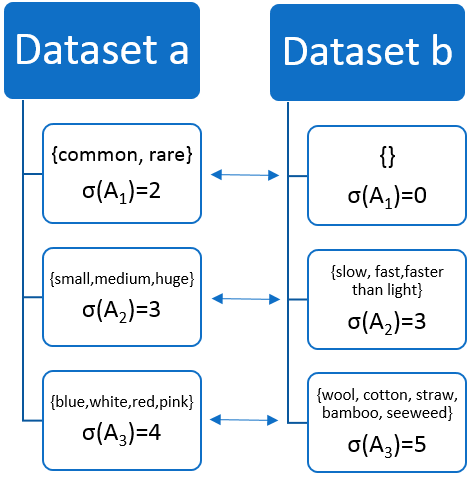
\includegraphics[width=7cm]{Images/example1.png}
		\centering
	\caption{Method one - attributes of datasets $a$ and $b$ were aligned according to their $\sigma$.}		\label{fig:example1}	
\end{figure} 
Now enumerate every aligned pair and sum up the differences between sigma values of each pair. The total distance is $|2-0|+|3-3|+|4-5|=2+0+1=3$.

We will use the same distance measure and the same datasets to demonstrate Algorithm \ref{algo:hungarianAlgorithm}. Let us define $IAttributeDistance$ function by building a distance matrix. The values of the distance matrix are in Table \ref{table:distance matrix}.
\begin{table}[htbp]
\caption{Distance matrix of the attributes of datasets $a$ and $b$. The matrix will serve as an input of the Hungarian algorithm.}
\label{table:distance matrix}
\centering
\begin{tabular}{ |c | c | c |c | }
  \hline
  & $a$ - $Att1$ & $a$ - $Att2$ & $a$ - $Att3$  \\
  \hline                       
  $b$ - $Att1$ & 1 & 2 & 3  \\
  $b$ - $Att2$ & 1 & 0 & 1  \\
  $b$ - $Att3$ ($\dummy$) & 4  & 3 & 2  \\  
  \hline  
\end{tabular}
\end{table}

By applying the Hungarian algorithm, we obtain the optimal alignment. The optimal alignment can be found in Table \ref{table:distancematrix2}.
\begin{table}
\caption{Results of application of the Hungarian algorithm. The optimal alignment is coloured.}
\label{table:distancematrix2}
\centering

\begin{tabular}{ |c | c | c |c | }
  \hline
  & $a$ - $Att1$ & $a$ - $Att2$ & $a$ - $Att3$  \\
  \hline                       
  $b$ - $Att1$ & \cellcolor{blue!25}1 & 2 & 3  \\
  $b$ - $Att2$ & 1 &\cellcolor{blue!25}0 & 1  \\
  $b$ - $Att3$ ($\dummy$) & 4  & 3 & \cellcolor{blue!25}2  \\
    \hline  
\end{tabular}
\end{table}

Algorithm \ref{algo:combinedAlignmentHungarian} adds selectors to the process. Imagine we have dataset $c$ defined in Table \ref{table:datasetc}. Suppose we have two selectors -- one for numerical and one for categorical attributes. New datasets emerge from the input dataset according to the selectors. In the case of dataset $c$ processed by the selectors, we will get two datasets. The first consisting solely of $Att1$ for the numerical selector and the second consisting solely of $Att2$ for the categorical selector.
This gives us a new assignment task for every selector. Such tasks are processed by attribute assignment algorithm (Algorithm \ref{algo:hungarianAlgorithm}) demonstrated above.
The algorithm finishes by weighting the inputs for each assignment result according to the given weights.

 \begin{table}[htbp]
	\caption{Possible values of dataset $c$.}
	\label{table:datasetc}
	\centering
	\begin{tabular}{ |c | c | c |c | }
		\hline
		$Att1$ & $Att2$  \\
		\hline                       
		1 &  Good \\
		4.5 &  Better \\
		3.7 &  Best \\
		5 &    \\
		2 &    \\
		\hline  
	\end{tabular}
\end{table} 

\subsubsection{Complexity Concerns}
The complexity of the assignment may be of a concern -- even though Hungarian algorithm is polynomial, its power can be too high. We do not expect this to be the case very often, since the model training usually takes quite a long time (for example, the problem of training the Neural Network with 3 hidden neurons is an NP-Complete problem \cite{neuralNetworkNPC}). Polynomial complexity for the recommendation is still just a negligible part of the whole process that can significantly reduce time of the training phase. Still, we would like to address the issue in case the complexity would be of concern. The complexities above are related to quality assessment of some algorithm. This is relevant when training new models, as the model assessment is part of the training. In the case of recommendation system being in production and new dataset arrives, the dataset distance is not needed for every pair of datasets but rather for the input and every other dataset. In case of the attribute assignment, the main burden lies in the Hungarian Algorithm.
%?Tarjan, Gabow - bounded
This can be mimicked by using approximate algorithms to solve the assignment problem:

\begin{definition}
Let $w(M)$ denote the weight of a matching in G, and $M^*$ a minimum-cost perfect matching in G. We call a perfect matching M \emph{$c$-approximate}, for $c \ge 1$, if $w(M) \le cw(M^*)$. 	
\end{definition}
In case the underlying matrix for assignment is a metric, we can use results of \cite{AgarwalApproximateBipartiteMatchingForMetric}. For any $\sigma > 0$, the authors present an algorithm that, in $$\mathcal{O}(n^{2+\sigma} \log n\log^2(1/\sigma))$$ time, computes a $\mathcal{O}(1/\sigma^\alpha)$-approximate matching of G, where $\alpha = \log_32 \approx 0.631$. 

\section{Theoretical Properties}
\label{section:theoreticalProperties}
In this section, we will explore interesting properties of the algorithms proposed in the previous section. We will show how the Assignments algorithm preserves metric properties, whether the same holds in opposite directions, and also we will be arguing about the best way of extending an attribute space with a $\dummy$ attribute.

Before we proceed to exploring the theoretical properties, we have to address a technicality. Consider the following situation. If the $\dummyinside$ is taken directly from the attribute space, it may theoretically happen that $\dummyinside$ will be compared to the equal attribute that was not dummy. However, to have at least a hope of obtaining a metric, we have to consider the case where the dataset with some attributes equal to $\dummyinside$ will be compared to almost the same dataset except that it will be missing the $\dummyinside$ attributes. The metric would require the distance between these datasets to be a non-zero. We have two ways to overcome this. We can also consider datasets equal if their attribute metadata are equal except any number of $\dummyinside$ like attributes. Another possibility is to modify the algorithm to distinguish between an artificial  $\dummyinside$ attribute and equal regular one and output some small non-negative number $\epsilon$ instead. At the same time, we would return $\epsilon + \attributeDistance(x,y)$ for non-matching input.
 In here we will use the former approach, as it will not clutter the text. However, we do not expect that this situation will happen often (or happen at all) as the attribute space will usually be of infinite size. 

\begin{theorem}
	\label{theorem:extendingOfAlignment}
	Let a, b be lists of attributes, f optimal alignment between a and b. Attribute distance measure $\attributeDistance$ is a metric on the extended space of attributes. Let $a' = a \cup \{\dummy_1\}$ and $b' = b \cup \{\dummy_2\}$, then $f'$ defined as 
	\begin{equation*}
	f'(x)=
	\begin{cases}
	f(x); \mbox{ if } x \in a, \\
	\dummy_2; \mbox{ otherwise}.
	\end{cases}
	\end{equation*}
	 is an optimal alignment between $a'$ and $b'$ with the same cost as f. This assignment extension is depicted in 
	 Figure \ref{fig:assignmentExtension}. 
	 \begin{figure}	
	 	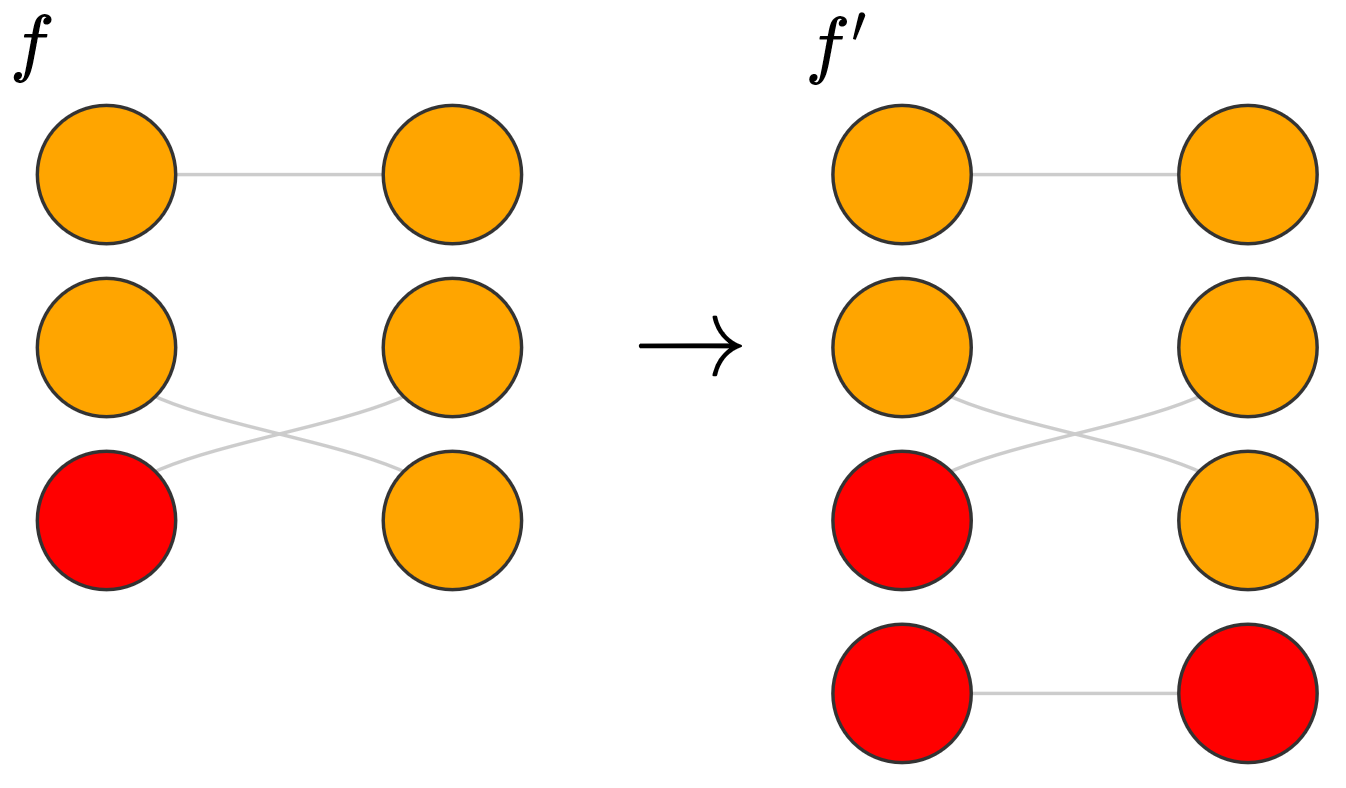
\includegraphics[width=7cm]{Images/assignmentExtension.png}
	 	\centering
	 	\caption{Extending optimal assignment by row of dummy attributes without changing the cost.}		\label{fig:assignmentExtension}	
	 \end{figure}
	\begin{proof}
		Suppose $f'$ is not an optimal assignment between $a'$ and $b'$ and some $f^*$ is. Observe that cost of $f'$ is the same as cost of $f$ because $\attributeDistance(\dummy_1, \dummy_2)=0$. Choose z so that $f^*(\dummy_1)=z$. If z is a dummy attribute, we can modify $f^*$ to $f'^*$ by swapping z and $\dummy_2$. Therefore $f'^*(\dummy_1)=\dummy_2$. As both $z$ and $\dummy_2$ are dummy attributes, this will not affect the cost of $f^*$. If $f'^*$ has lower cost than $f'$ (and thus consequently $f$), we can improve original $f,$ which is a contradiction. If it has the same cost then $f'$ must have been optimal which is also the contradiction. 
		
		The remaining case is that z is not dummy. Let k be $f^{*-1}(\dummy_2)$. Modify $f^*$ as follows:
		\begin{equation*}
		f'^*(x)=
		\begin{cases}
		z; \mbox{ if } x = k, \\
		\dummy_2; \mbox{ if } x = \dummy_1, \\
		f^*(x); \mbox{ otherwise}.
		\end{cases}
		\end{equation*}
		Let us examine cost of $f'^*$. We want to prove that this modification of $f^*$ to $f'^*$ did not increase the cost. As everything is the same except $\dummy_1$ and $k$, we need to investigate only those. We want to prove that $$\attributeDistance(k,z) + \attributeDistance(\dummy_1, \dummy_2) \le \attributeDistance(k,\dummy_2) + \attributeDistance(\dummy_1, z).$$
		Using the coincidence axiom the above is equivalent to
		$$\attributeDistance(k,z) \le \attributeDistance(k,\dummy_2) + \attributeDistance(\dummy_1, z)$$
		as $\attributeDistance(\dummy_1, \dummy_2)=0.$ This is of course true because it is an instance of triangle inequality.
	
 Now we can make the same argument we did with the z being a dummy attribute: If $f'^*$ has lower cost than $f'$ (and thus consequently $f$), we can improve original $f,$ which is a contradiction. If it has the same cost then $f'$ must have been optimal, which is also the contradiction. In all cases, $f'$ must have been optimal alignment.
	\end{proof}
\end{theorem}
By applying this theorem multiple times, we can add an arbitrary number of $\dummy$ attributes without changing the optimality of alignment.
\begin{theorem}
	\label{theorem:metricPreservation}
	Let a, b are list of attributes, $\attributeDistance$ is a metric on the extended space of attributes. Then Algorithm \ref{algo:attributeAlignmentHungarian} preserves all metric axioms and resulting distance $\globalDistance$ on the dataset space is a metric.
	\begin{proof} We will split the proof according to the different metric axioms.
	\begin{enumerate}
		\item We will begin with proving the non-negativity axiom. Since $\attributeDistance$ is a metric, it satisfies non negativity axiom. The cost of the minimal assignment must be non-negative as well.
		\item For the coincidence axiom we have to prove both direction of the equivalence:
		 \begin{itemize}
			\item $\Rightarrow:$ If $\globalDistance(x,y)=0$, the cost of minimal assignment was $0$. As $\attributeDistance$ satisfies non-negativity, it must be the case that all attributes were equal since $\attributeDistance$ also satisfies coincidence axiom. As all attributes were equal, the $x$ and $y$ must also be equal (up to permutation).
			\item $\Leftarrow:$ If $x=y$, all attributes must be equal (up to a permutation). Optimal solution is for every attribute assign the equal attribute. As $\attributeDistance$ satisfies coincidence and non-negativity, this optimal solution cost is 0.		
		\end{itemize}
		\item The proof of the symmetry axiom is as follows: given two datasets $a$ and $b$,
		the $a$ and $b$ are either of the same cardinality or the dataset with fewer attributes is extended by the appropriate number of  $\dummy$ attributes, so the cardinalities of the datasets match. This is done regardless of the order of the arguments. Therefore, for the rest of this part, we can assume that the dataset have the same number of attributes. Hungarian algorithm would find an optimal alignment $f$ -- a bijection from $a$ to $b$. If we would switch the arguments, algorithm would find the optimal bijection $g$ from $b$ to $a$.
		However, in both cases the algorithm would optimize the same thing, therefore the $\text{cost}(f) = \text{cost}(g)$, which would be the output of the algorithms regardless of their order.
		\item The remaining axiom to prove is the triangle inequality axiom. Let $x,y$ and $z$ be arbitrary datasets, $\attributeDistance$ metric on the attribute space and $\globalDistance$ dataset distance measure produced by the algorithm. We want to prove that $\globalDistance(x,y)\le \globalDistance(x,z) + \globalDistance(z,y).$ The algorithm would produce optimal assignments $f,g$ and $h$ between $x',y'$, $x,z$ and $z, y$ respectively. We can reformulate our goal to proving that  $\text{cost}(f) \le \text{cost}(g) +  \text{cost}(h).$ If the cardinality of the datasets would not match the corresponding amount of $\dummy$ attributes would be added to the datasets for the sake of the assignments. Now we will take maximum cardinality of the domains of the assignments:  $$max_{card}=\max(\mathbf{card}(\text{domain}(f),\mathbf{card}(\text{domain}(g),\mathbf{card}(\text{domain}(h)).$$
		
		We will now extend the datasets by adding extra $\dummy$ attributes so the number of attributes matches the $max_{card}.$ We get datasets $x', y'$ and $z'$.
		Corresponding new optimal assignments would be $f',g'$ and $h'$. We will argue that we did not change the costs of the assignments. If needed, algorithm would first add the $\dummy$ attributes to get the original assignments. If the domain does not match the $max_{card}$ we could use Theorem \ref{theorem:extendingOfAlignment}. With its help we could add the desired amount of $\dummy$ attributes finally reaching to extended datasets and another optimal assignment with the same cost as the original one. Note that the following now holds: $$\mathbf{card}(\text{domain}(f')=\mathbf{card}(\text{domain}(g')=\mathbf{card}(\text{domain}(h')).$$
		
		We proceed with creating the suboptimal assignment $f^\circ$ from $\text{domain}(f')$ to $\text{range}(f')$ by function composition of $g'$ and $h'$ -- $f^\circ=h'\circ g'$. We can do that as $\text{domain}(f')=\text{domain}(g')$ and $\text{range}(f')=\text{range}(h')$. As $f'$ is optimal we get 
		$$\text{cost}(f)=\text{cost}(f') \le \text{cost}(f^\circ)=
		\sum_{i=1}^{\text{len}(x')}\attributeDistance(x[i],f^\circ(x[i])).$$ 
		According to the fact that $\attributeDistance$ satisfies triangle inequality and the fact that $f^\circ=h'\circ g'$ we get
		$$\sum_{i=1}^{\text{len}(x')}\attributeDistance(x[i],f^\circ (x[i])) \le 
		\sum_{i=1}^{\text{len}(x')}(\attributeDistance(x[i],g'(x[i]))+ \attributeDistance(g'(x[i]),h'(g'(x[i])))).$$
		As $\text{range}(g')=\text{domain}(h')$ and every assignment function is a bijection, summing over elements of $x'$ is the same as summing over the permutation of elements of $x'$ given by assignments, we can conclude the proof:
		\begin{align*}
		\sum_{i=1}^{\text{len}(x')}(\attributeDistance(x[i],g'(x[i]))+ \attributeDistance(g'(x[i]),h'(g'(x[i]))))&=\text{cost}(g')+\text{cost}(h') \\
		& =\text{cost}(g)+\text{cost}(h).
		\end{align*}			 
		The whole proof of the triangle inequality is illustrated in Figure \ref{fig:metricPreservation}. 
		\begin{figure}	
			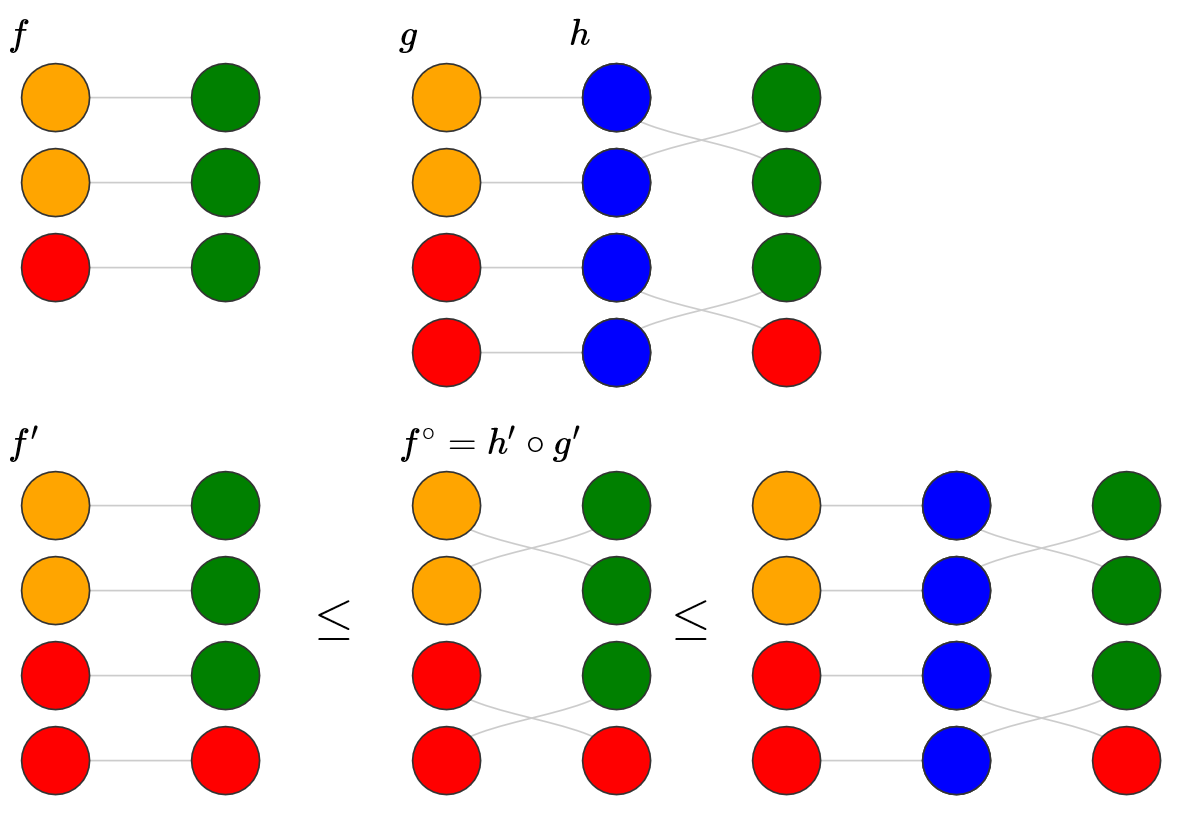
\includegraphics[width=14cm]{Images/metricPreservation.png}
			\centering
			\caption{Proof of Theorem \ref{theorem:metricPreservation} -- metric axiom 4 is preserved. Alignment $f$ is extended and then reshuffled so the triangle inequality can be applied. Yellow nodes are original attributes of dataset $x$, green nodes are attributes of dataset $y$ and blue of dataset $z$. Red nodes are $\dummy$ attributes used for extending the datasets so the corresponding assignments are of the same cardinality.}	
			\label{fig:metricPreservation}	
		\end{figure}
	\end{enumerate} 	
	As all metric axioms are proven, we can conclude the proof.	
	\end{proof}
\end{theorem}

The previous theorem also holds for Algorithm \ref{algo:combinedAlignmentHungarian}:
\begin{corollary}
		\label{corollary:metricPreservation}
		Let a, b are lists of attributes, $\{\attributeDistance_1, \dots, \attributeDistance_n \}$ are metrics on the extended space of attributes, $\{s_1, \dots, s_n\}$ are selectors, $\{w_1, \dots, w_n\}$ are positive weights of each selector. Then Algorithm \ref{algo:combinedAlignmentHungarian} preserves all metric axioms and resulting distance on the dataset space is a metric.	
	\begin{proof}
		Follows from the previous theorem and the fact that sum of metrics with positive weights is also a metric (Corollary \ref{corollary:weightedMetricAddition}).
	\end{proof}
\end{corollary}

It may be interesting to see how to extend attribute space by an artificial $\dummyoutside$ attribute. A following theorem gives us some clue: 
\begin{theorem}
	\label{theorem:dummyConstantMinimalDistance}
		Let $\attributeDistance'$ be a metric on a non-empty attribute space $\mathbb{A}$.	Let $\attributeDistance$ be a distance derived from $\attributeDistance'$ by extending  $\mathbb{A}$ by artificial $\dummyoutside$ attribute. We set the $\attributeDistance(\dummyoutside, x)$ and $\attributeDistance(x, \dummyoutside)$ to some constant $k$ $\forall x \in \mathbb{A}$. Finally, we set $\attributeDistance(\dummyoutside, \dummyoutside)=0.$ Let $\attributeDistance_{max}=\max_{x,y \in \mathbb{A}}\attributeDistance(x,y).$ If $\attributeDistance$ is a metric on the extended attribute space then $0 < k$ and $\frac{\attributeDistance_{max}}{2} \le k$.	
	\begin{proof}
		If $k < 0$ then $\attributeDistance(\dummyoutside, x)<0$, which would contradict non-negativity. If $k = 0$ then $\attributeDistance(\dummyoutside, x)=0$ and for every $x \in \mathbb{A}$ is $x \ne \dummyoutside$, which contradicts coincidence axiom.   
	The idea of the remaining part is as follows: we cannot short-cut our way when going on the longest way in the space by going through $\dummyoutside$ attribute which has the constant distance from every other point in the space -- this is depicted in Figure \ref{fig:constDummyTheorem}. 
	\begin{figure}	
		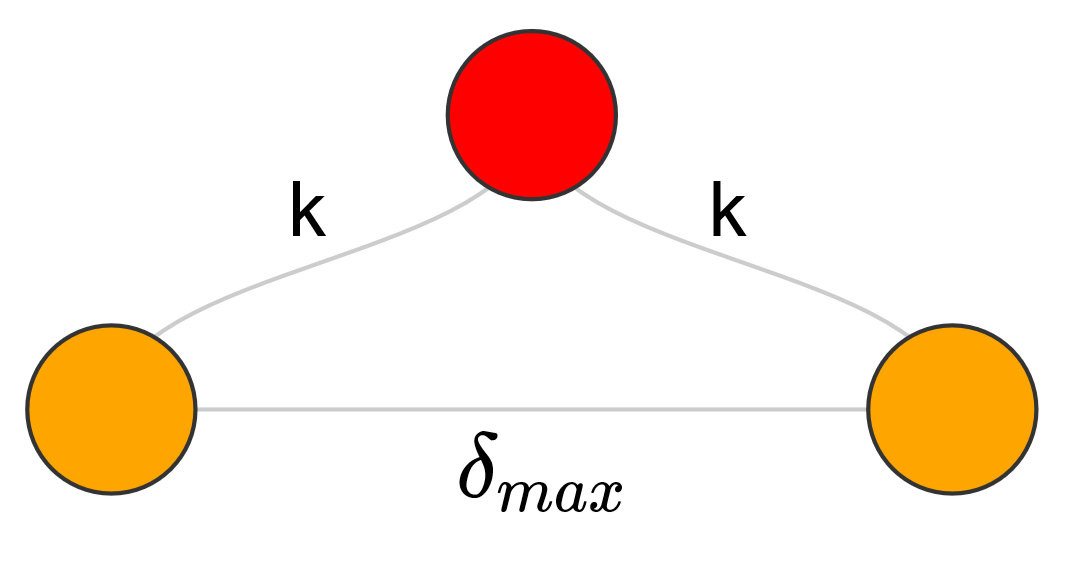
\includegraphics[width=7cm]{Images/constDummyTheorem.png}
		\centering
		\caption{Part of proof of Theorem \ref{theorem:dummyConstantMinimalDistance}. Constant $k$ representing a distance between a regular and an artificial  $\dummyoutside$ attribute  needs to be big enough in order not to create the shortcut between the most distant points.}	
		\label{fig:constDummyTheorem}	
	\end{figure}
	Find $x_0, y_0$ so that $\attributeDistance(x_0,y_0)=\attributeDistance_{max}$. From triangle inequality we get $ \forall x,y \in \mathbb{A}: \attributeDistance(x,y) \le \attributeDistance(x, \dummyoutside) + \attributeDistance(\dummyoutside, y)$. All the more true that $\attributeDistance(x_0,y_0) \le \attributeDistance(x_0, \dummyoutside) + \attributeDistance(\dummyoutside, y_0)$. As $\forall z \in \mathbb{A}:  \attributeDistance(\dummyoutside, z) = \attributeDistance(z, \dummyoutside) = k$ we get $\attributeDistance_{max} \le 2k$ which is equivalent to $\frac{\attributeDistance{max}}{2} \le k$.	
	\end{proof}
\end{theorem}
If we want to have metric attribute distance, and at the same time, a constant distance from artificial $\dummyoutside$ attributes, we have to choose this constant from quite large values. Doing this can create unwanted side affects. The penalty for adding $\dummyoutside$ attributes can become the most significant part of the distance, especially if the number of attributes varies by large amounts. It can be argued that if some attributes are not very relevant for the prediction of the target (for example attributes with low entropy), the two datasets should not differ too much if one dataset is missing such not very relevant attributes. Furthermore, in some cases it may be impossible to compute $\delta_{max}$ or to learn the value in advance. 

We get no such problems if we use the element of the attribute space itself, if we already made sure that the attribute distance is a metric. Using the $\dummyinside$ attribute from the space will not break the metric axioms (if the attribute distance $\attributeDistance$ is a metric).

Theorem \ref{theorem:metricPreservation} is also valid in the opposite direction, as shown in the following theorem.
\begin{theorem}
	\label{theorem:metricRestoration}
	Let a, b are list of attributes, $\attributeDistance$ is a distance between attributes. If $\globalDistance$ is a distance over dataset space produced by Algorithm \ref{algo:attributeAlignmentHungarian} and $\globalDistance$ is a metric on the dataset space, then $\attributeDistance$ is a metric on the extended attribute space $\mathbb{A}$.
	\begin{proof} Again, we will split the proof according to the different metric axioms.
		\begin{enumerate}
			\item We will begin with proving the non-negativity axiom. 	For the sake of contradiction, let us suppose that $\attributeDistance$ does not satisfy non-negativity axiom. It must be the case that $\exists x,y \in \mathbb{A}$ so $\attributeDistance(x,y) < 0$. We define datasets $X$ and $Y$ consisting solely of $x$ and $y$ respectively. There is only a single assignment $f$ available -- mapping $x$ to $y$ and is therefore optimal. Algorithm \ref{algo:attributeAlignmentHungarian} will output the $\text{cost}(f)$:  $\globalDistance(X,Y)\sum_{i=1}^{1}\attributeDistance(X[i],f(X[i]))=\attributeDistance(x,y)$. We get a contradiction as $\globalDistance(X,Y) \ge 0$ and $\attributeDistance(x,y) < 0$.
			\item For the coincidence axiom we have to prove both direction of the equivalence:
			\begin{itemize}
				\item $\Rightarrow:$  If $\attributeDistance(x,y)=0 \land x \ne y$, we define datasets $X$ and $Y$ consisting solely of x and y respectively. $X \ne Y$ and as $\globalDistance$ is a metric we get $\globalDistance(X,Y) > 0$. As $\mathbf{card} (X) = \mathbf{card} (Y)=1$ there is only a single assignment $f$ available and must be the optimal alignment returned by Algorithm \ref{algo:hungarianAlgorithm}. The cost outputted by Algorithm \ref{algo:attributeAlignmentHungarian} is $\globalDistance(X,Y)\sum_{i=1}^{1}\attributeDistance(X[i],f(X[i]))=\attributeDistance(x,y)=0,$ which is a contradiction.
				\item $\Leftarrow:$  If $x=y \land \attributeDistance(x,y)>0$  we define datasets $X$ and $Y$ consisting solely of x. $X = Y$ and as $\globalDistance$ is a metric we get $\globalDistance(X,Y) = 0$. As $\mathbf{card} (X) = \mathbf{card} (Y)=1$ there is only a single assignment $f$ available and must be the optimal alignment used by Algorithm \ref{algo:attributeAlignmentHungarian}. The cost outputted by the algorithm is $\globalDistance(X,Y)\sum_{i=1}^{1}\attributeDistance(X[i],f(X[i]))=\attributeDistance(x,y)>0,$ which is a contradiction.		
			\end{itemize}
			\item The proof ot the symmetry axiom is as follows. For the sake of contradiction, let us assume that $\attributeDistance$ does not satisfy symmetry axiom. It must be the case that $\exists x,y \in \mathbb{A}$ so $\attributeDistance(x,y) \ne \attributeDistance(y,x)$. We will define datasets $X$ and $Y$ consisting solely of $x$ and $y$ respectively. There is only a single assignment $f$ from $X$ to $Y$ available -- mapping $x$ to $y$ and is therefore optimal. Similarly, there is only a single assignment $g$ from $Y$ to $X$ available -- mapping $y$ to $x$ and is therefore optimal. Algorithm \ref{algo:attributeAlignmentHungarian} will output the $\text{cost}(f)$:  
			$$\globalDistance(X,Y)\sum_{i=1}^{1}\attributeDistance(X[i],f(X[i]))=\attributeDistance(x,y).$$
			The $\text{cost}(g)$ is computed analogically: $$\globalDistance(Y,X)\sum_{i=1}^{1}\attributeDistance(Y[i],g(Y[i]))=\attributeDistance(y,x).$$ 
			We get a contradiction. As $\globalDistance$ satisfies symmetry axiom we get $\globalDistance(X,Y) = \globalDistance(Y,X)$. However, at the same time we have $\globalDistance(X,Y) \ne \globalDistance(Y,X)$ from assumptions.
			\item The remaining axiom to prove is the triangle inequality axiom. For the sake of contradiction, let us suppose that $\attributeDistance$ does not satisfy triangle inequality. It must be the case that $\exists x,y,z \in \mathbb{A}$ so $\attributeDistance(x,y) > \attributeDistance(x,z)+\attributeDistance(z,x)$. We will  define datasets $X$, $Y$ and $Z$ consisting solely of $x$,$y$ and $z$ respectively. There is only a single assignment $f$ from $X$ to $Y$ available -- mapping $x$ to $y$ and is therefore optimal. Similarly, there is only a single assignment $g$ from $X$ to $Z$ available and only a single assignment $h$ from $Z$ to $Y$ -- both are also optimal. Algorithm \ref{algo:attributeAlignmentHungarian} will output the $\text{cost}(f)$:
			$$\globalDistance(X,Y)\sum_{i=1}^{1}\attributeDistance(X[i],f(X[i]))=\attributeDistance(x,y).$$
			Again, the $\text{cost}(g)$ and $\text{cost}(h)$ are computed analogically:
			\begin{equation*}
			\globalDistance(X,Z)\sum_{i=1}^{1}\attributeDistance(X[i],g(X[i]))=\attributeDistance(x,z),
			\end{equation*}
			\begin{equation*}
			\globalDistance(Z,Y)\sum_{i=1}^{1}\attributeDistance(Z[i],h(Z[i]))=\attributeDistance(z,y).
			\end{equation*}
			 As $\globalDistance$ satisfies triangle inequality we have $\globalDistance(X,Y) \le \globalDistance(X,Z)+\globalDistance(Z,Y).$ At the same time we have $\globalDistance(X,Y) > \globalDistance(X,Z)+\globalDistance(Z,Y)$ from assumptions, which is a contradiction.
		\end{enumerate}
			As all metric axioms are proven, we can conclude the proof.	
		\end{proof}	
\end{theorem}

Similar theorem holds for Algorithm \ref{algo:combinedAlignmentHungarian} with addition that all selectors must be distinct:
\begin{corollary}
		\label{corollary:metricRestoration}
		Let a, b are list of attributes, $\{\attributeDistance_1, \dots, \attributeDistance_n\}$ are the distances on the extended space of attributes, $[s_1, \dots, s_n]$ are selectors, $[w_1, \dots, w_n]$ are weights of each selector. If $\forall k,j \in \left\{1, \dots, n\right\}, \forall \mathbb{A'} \subseteq \mathbb{A}:s_k(\mathbb{A'})\bigcap s_j(\mathbb{A'})= \emptyset$ and distance $\globalDistance$ produced by Algorithm \ref{algo:combinedAlignmentHungarian} is a metric on the dataset space then $\{\attributeDistance_1, \dots, \attributeDistance_n\}$ are metrics on the extended attribute space defined by the corresponding selector.	
	\begin{proof}
		We can prove the corollary by following the proof of the previous theorem. When creating dataset of a single element, we now do this for every $\attributeDistance_i$ that does not satisfy axiom in question. As selectors are distinct, other selectors will return $\emptyset$ from single element datasets and therefore will output 0 for corresponding selector distance, as the resulting distance is the sum over all attributes returned by the selector.
	\end{proof}
\end{corollary}
It is intuitive to have each selector distinct, if we think of a selector in the sense we have introduced them: selector selects specific attributes (e.g. categorical or numerical) so more fine grained distance functions can be applied. In this sense the selectors will be distinct as the subset of categorical attributes is clearly disjunct to subset of numerical attributes.

We can wonder whether Corollary \ref{corollary:metricRestoration} holds even without the constraint for distinct selectors. 
\begin{observation}
The requirement for distinct selectors is an essential part of Corollary \ref{corollary:metricRestoration}. 
\begin{proof}
	We will show a counterexample: let attribute space be the set of two elements: $\mathbb{A}={a_1, a_2}$.
	Let $s_1,s_2$ be two selectors defined as $s_1(\mathbb{X})=s_2(\mathbb{X})=\mathbb{X}$. Let $\attributeDistance_1$ be a metric and $\attributeDistance_2$ be a distance function defined as $\attributeDistance_2(x,y)=-0.1\attributeDistance_1(x,y)$. $\attributeDistance_2$ is not a metric on the attribute space as it violates non-negativity -- $\attributeDistance_2(a_1, a_2) = -0.1\attributeDistance_1(a_1, a_2) < 0$. It still satisfies symmetry and coincidence though. We can combine $\attributeDistance_1$ and $\attributeDistance_2$ to form $\attributeDistance_3$: $\attributeDistance_3(x,y) = \attributeDistance_1(x,y)+\attributeDistance_2(x,y)=0.9\attributeDistance(x,y)$. $\globalDistance$ induced by $\attributeDistance_1$, $\attributeDistance_2$, and $s_1 = s_2$ is the same as $\globalDistance'$ induced by $\attributeDistance_3$. $\attributeDistance_3$ is a metric on the attribute space according to Theorem \ref{theorem:metricrescaling} as it is positively rescaled $\attributeDistance_1$. Therefore, it does not matter if we use the combination of $\attributeDistance_1,\attributeDistance_2$ or just $\attributeDistance_3$ alone. Resulting $\globalDistance$ is a metric on the dataset space according to Theorem \ref{theorem:metricPreservation} even-though $\attributeDistance_2$ is not a metric on the dataset space.
\end{proof}
\end{observation}

Theorems \ref{theorem:metricPreservation}, \ref{theorem:metricRestoration} and Corollaries \ref{corollary:metricPreservation} and  \ref{corollary:metricRestoration} are useful as they state that if we can get a metric on the attribute or dataset space, we get other metric on the other space for free when using attribute aligning. During training, we could define a function measuring metric similarity on the attribute or dataset samples. As the samples would usually be just small finite subsets of attribute or datasets space, we could be wondering whether by optimizing metric on some dataset or attribute subset, we would get also metric on the other subset as Theorems \ref{theorem:metricPreservation}, \ref{theorem:metricRestoration} and Corollaries \ref{corollary:metricPreservation}, \ref{corollary:metricRestoration} are valid only for the whole spaces. We will try to formalize this motion:

\begin{definition}
\label{definition:supportedDatasets}
Let $\mathbb{A}$ be attribute space, let $A$ be the subset of $\mathbb{A}$. Let $\mathbb{D}$ be a dataset space. Then we will denote dataset subspace $D$ as \emph{supported} by attribute subspace $A$ if $D \subseteq \mathbb{D}$ and if $\forall d \in D,\forall att \in d:att \in A$. 
\end{definition} 
In other words, datasets in $D$ are only composed of elements in $A$. This definition allow us to investigate metric properties in just the subset of attribute spaces and conclude properties in supported subspaces of datasets (like training and testing subset) and vice-versa.

\begin{definition}
Let $\mathbb{A}$ be attribute space, let $\mathbb{D}$ be a dataset space and $D$ its subset. We will call the subset $A$ of $\mathbb{A}$ as the \emph{source} of $D$ if $\forall att \in \mathbb{A}: att \in A \iff \exists d \in D: att \in d$. 
\end{definition} 
In other words, elements of $A$ are just enough in order to create all elements in $D$. Similarly to the remark to Definition \ref{definition:supportedDatasets}, we can use this definition to reason about whether properties that are valid for some distance function on some set of datasets are also valid for the attribute source of these datasets.

If we optimize metric on subset of attributes, we also get metric on all datasets that can be combined by this subset of attributes when using Algorithm \ref{algo:attributeAlignmentHungarian}:
\begin{theorem}
\label{theorem:metricPreservationSuportedSpaces}
Let $\mathbb{A}$ be extended space of attributes and $A$ its extended subset, $\attributeDistance$ is a metric on $A$, $\mathbb{D}$ space of datasets. Then $\forall D \subseteq \mathbb{D}$, $D$ supported by $A$: Algorithm \ref{algo:attributeAlignmentHungarian} preserves all metric axioms and resulting distance $\globalDistance$ on the $D$ is a metric.
	\begin{proof}
	From following the proof of Theorem \ref{theorem:metricPreservation} as the proof does not require elements outside of $D$ or $A$ and we can replace the whole $\mathbb{D}$ by $D$ and $\mathbb{A}$ by $A$.
	\end{proof}
\end{theorem}
Intuitively, the same works for Algorithm \ref{algo:combinedAlignmentHungarian}.

This enables us to define our algorithms in such a way, that if we can create a metric on all the attributes in the training and testing samples, we can also guarantee the resulting metric on all supported subsets of the dataset space. The training and testing datasets must be among them, as they are supported by the testing and training attributes.

Note that Theorem \ref{theorem:metricPreservationSuportedSpaces} is valid because there is nothing in the proof of Theorem~\ref{theorem:metricPreservation} that would require elements (datasets) outside of the subset $D$ and $A$. As for the other direction,  when observing the proof of Theorem \ref{theorem:metricRestoration}, we use the trick that we artificially create datasets with a single element. However, such datasets can be outside of $D$. We can then wonder whether Theorem \ref{theorem:metricPreservationSuportedSpaces} is valid also in the other direction considering  Algorithm \ref{algo:attributeAlignmentHungarian}. It is not according to Observation~\ref{theorem:metricNonRestorationSupportedSpaces}.

\begin{observation}
	\label{theorem:metricNonRestorationSupportedSpaces}
	Let $\mathbb{A}$ be space of attributes and $\mathbb{D}$ space of datasets. Let $D$ be a subset of $\mathbb{D}$ and $\globalDistance$ a metric on $D$. Let $A$ be the source of $D$ and $\attributeDistance$ be a distance measure on $A$, such that Algorithm \ref{algo:attributeAlignmentHungarian} induces $\globalDistance$ using $\attributeDistance$. Then $\attributeDistance$ is not necessarily a metric on $A$.
	\begin{proof}
	We will show a counterexample.
	Let $\mathbb{A}$ be the space of attributes, $D$ be the subspace of datasets  consisting of single dataset $d=\left\lbrace a_1, a_2, a_3 \right\rbrace$. Let $A=\left\lbrace a_1, a_2, a_3 \right\rbrace \subseteq \mathbb{A}$ the source of $D$. Let $\globalDistance$ be a metric on  $D$. Since $D$ consists of only one element, in order $d$ to be a metric all we need to do is set $\globalDistance(d,d)=0$. Let $\attributeDistance$ be attribute distance function on $A$. We will show that even though $\globalDistance$ is a metric, $\attributeDistance$ does not have necessarily to be a metric. We can define $\attributeDistance$ as shown in Table \ref{table:supportAttributeCounterexample}. As there are some negative values, the attribute distance $\attributeDistance$ is not a metric.
	\begin{table}
		\caption{Counterexample that metric on some subspace of datasets does not imply metric on its source attribute subspace}
		\label{table:supportAttributeCounterexample}
		\centering
		\begin{tabular}{ |c | c | c |c | }
			\hline
			& $a_1$ & $a_2$ & $a_3$  \\
			\hline                       
			$a_1$ & \cellcolor{blue!25} 0 & 50 & 50  \\
			$a_2$ & 50 &\cellcolor{blue!25}-5 & 50  \\
			$a_3$ & 50  & 50 & \cellcolor{blue!25}5  \\
			\hline  
		\end{tabular}
	\end{table}
	The optimal alignment $f$ between $d$ and $d$ is coloured and is defined as $f(a_i)=a_i$.
	The $\text{cost}(f)=\attributeDistance(a_1,a_1)+\attributeDistance(a_2,a_2)+\attributeDistance(a_3,a_3)=0+5-5=0=\globalDistance(d,d)$.
	\end{proof}
\end{observation}

Same counterexample can be found when using Algorithm \ref{algo:combinedAlignmentHungarian} as this algorithm is a generalization of Algorithm \ref{algo:attributeAlignmentHungarian}, therefore the same argument can be applied. 
This implies that we cannot guarantee metric on the subspace of attributes appearing in the training and testing datasets even if we can guarantee resulting distance to be a metric on the training and testing dataset subspace.

Another argument favouring a metric for the attributes is that specialized algorithms can be used for the assignment such as \cite{AgarwalApproximateBipartiteMatchingForMetric}.

\section{Distance Using Attribute Metadata}
In Section \ref{section:distanceUsingGlobalMetadata}, we discussed distance based on a vector of global metafeatures. We can analogically define a distance on the attribute space or subspace defined by some selector. This can be then the $IAttributeDistance$ input for Algorithms \ref{algo:attributeAlignmentHungarian} and \ref{algo:combinedAlignmentHungarian}.

\IncMargin{1em}
\begin{algorithm}
\SetKwInOut{Input}{input}
\SetKwInOut{Output}{output}
\tcp{Pseudocode for measuring distance between attribute treating attributes as real valued vector.}
\Input{$\sigma$ $\leftarrow$ Vector distance measure}
\Input{$x \leftarrow$ First attribute}
\Input{$y \leftarrow$ Second attribute}
\Output{Distance between two attributes}
\BlankLine
$\text{vector}_x \leftarrow x_{\text{attribute\_metafeatures}}$\;
$\text{vector}_y \leftarrow y_\text{attribute\_metafeatures}$\;
distance $\leftarrow \sigma(\text{vector}_x,\text{vector}_y)$\;
\Return $distance$\;
\caption{Vectorized Attribute Distance: $IAttributeDistance$}\label{algo:basicAttributeDistance}
\end{algorithm}\DecMargin{1em}
\emph{Attribute\_metafeatures} is a property returning real value vector of attribute metafeatures for a given attribute.
This property does not have to be necessarily defined on the whole attribute space. For example, in the case of Algorithm \ref{algo:combinedAlignmentHungarian} it must be defined only on the subspace of attributes defined by the corresponding selector, e.g. it can return vector of features specific for numerical attributes in the case of numerical selector.


Again, note that both variables $\text{vector}_x, \text{vector}_y$ are real valued vectors of the same length $n$. This allows us to use any metric defined on $\mathbb{R}^n$ including all the metrics based on $p$-norms (Theorem \ref{theorem:pnormisnorm}) and their weighted counterparts (Theorem~\ref{theorem:weightedpnormisnorm}) and the resulting attribute measure will also be a metric. Using such metric in Algorithms \ref{algo:attributeAlignmentHungarian} and \ref{algo:combinedAlignmentHungarian} will preserve the metric and the resulting dataset distance will be also a metric according to Theorems \ref{theorem:metricPreservation} and \ref{theorem:metricPreservationSuportedSpaces}, and Corollary \ref{corollary:metricPreservation} and its selector counterpart.

\section{Combining the Distances}
We have dedicated lots of effort to utilize extra information from the attributes. We have the whole workflow that builds the distance on the datasets from the attribute distance through aligning and selectors. In this section, we would like to address the fact that global attributes store useful information as well -- this was proven in the literature. Even though the attribute alignment was competitive to global dataset distances, it does not necessarily mean that we have to use them separately from each other. In fact, it could be useful to combine their powers to get even better distance measure between datasets. In order to achieve this we have proposed Algorithm \ref{algo:datasetDistanceCombination}.

\IncMargin{1em}
\begin{algorithm}
\SetKwInOut{Input}{input}
\SetKwInOut{Output}{output}
\tcp{Pseudocode for combining multiple dataset distance measure and producing their weighted combination.}
\Input{distances $\leftarrow$ List of dataset distance measures $\globalDistance$}
\Input{weights $\leftarrow$ List of weights}
\Input{$x$ $\leftarrow$ First dataset}
\Input{$y$ $\leftarrow$ Second dataset}
\Output{Distance between two datasets}
\BlankLine
distance $\leftarrow 0$\;
\For{\upshape $i$ in $\lbrace 1,\dots, \text{len(distances)} \rbrace$}{
distance $\leftarrow$ distance + weights[$i$]distances[$i$]$(x,y)$\;
}
\Return distance\;
\caption{Dataset Distance Aggregation: $IDatasetDistance$}\label{algo:datasetDistanceCombination}
\end{algorithm}\DecMargin{1em}

This algorithm takes list of dataset distance measures and weights their results.
If the underlying datasets measures are metric and weights are positive, the algorithm will also produces a metric on the datasets space according to the fact that weighted sum of metrics is also a metric, if the weights are positive (Corollary \ref{corollary:weightedMetricAddition}).
As usual, using the $partial$ application we can conform to the $IDatasetDistance$ interface, if we fix all the arguments except the last two.

\section{Normalization Based on the Number of Attributes}
When using Algorithms \ref{algo:attributeAlignmentMasterThesis}, \ref{algo:attributeAlignmentHungarian} and \ref{algo:combinedAlignmentHungarian}, after getting the total distance defined by the optimal alignment, we could think about normalizing this distance by the number of attributes. This would amend the algorithms. Algorithm \ref{algo:attributeAlignmentHungarian} would return $\frac{TotalDistance}{NumberOfAttributes}$ instead. Algorithm \ref{algo:combinedAlignmentHungarian} would do this amendment for each selector (and number of attributes would be based on the number of attributes selected by the selector). Such amendments would normalize this distance to a count independent on the attribute number. This may or may not be beneficial, but in this section we show that there are theoretical reasons against it.

There are two natural ways how to normalize by the number of attributes. Given two datasets $a$ and $b$ with the number of attributes $|a|$ and $|b|$, we can either divide the total distance by $\min(|a|,|b|)$ or by $\max(|a|,|b|)$.
We will start by exploring the latter case -- $\max(|a|,|b|)$. Without the normalization, if the underlying attribute distance is a metric, the metric preservation to the dataset distance is ensured by Theorem \ref{theorem:metricPreservation}. We will show that this is not necessary true if we do the normalization according to the $\max(|a|,|b|)$.

\begin{observation}
	Normalizing the distance by $\max(|a|,|b|)$ can violate metric axioms.
	\begin{proof}
		Let $\attributeDistance$ be a metric on the extended attribute space $\mathbb{A}$, $\dummy \in \mathbb{A}$, $a=\lbrace a_1 \rbrace,b= \lbrace b_1 \rbrace$ are datasets. Let us define the $\attributeDistance(a_1,b_1)$ as 1 and set $\attributeDistance(a_1,\dummy)=\attributeDistance(b_1,\dummy)=10$. The optimal alignment is the only one possible, $\max(|a|,|b|)$ is 1, therefore distance $\globalDistance$ returned by the normalized Algorithm \ref{algo:attributeAlignmentHungarian} is $\frac{1}{1}$. We will show that the triangle inequality does not have to be preserved. We will define dataset $z$ as $\lbrace a_1,\dummy \rbrace$. For the triangle inequality to hold, it must be the case that $\globalDistance(a,b) \le \globalDistance(a,z)+\globalDistance(z,b)$. Let us see what $\globalDistance(a,z)$ is. One $\dummy$ attribute will be added, as $\attributeDistance(\dummy,\dummy)=0$, we get optimal alignment of the cost of zero as it will align $a_1$ to $a_1$ and $\dummy$ to $\dummy$. The zero will be divided by  $\max(|a|,|z|)$ resulting in $\globalDistance(a,z)=0$. As for the $\globalDistance(z,b)$, one $\dummy$ attribute is again added to $b$,  the optimal alignment is either $a_1 \rightarrow b_1, \dummy \rightarrow \dummy$ or $a_1 \rightarrow \dummy, \dummy \rightarrow b_1$. The cost of the former is 1, the cost of the latter is $2 \times 10=20$ . Therefore, the former is optimal. As $\max(|b|,|z|)=2$ we get $\globalDistance(z,b)=1/2$.
		Finally we get $1=\globalDistance(a,b) \le \globalDistance(a,z)+\globalDistance(z,b)=1/2$ which is not valid and distance on the dataset space $\globalDistance$ is not a metric, as the triangle inequality was broken.
	\end{proof}
\end{observation}

The same holds for the former case -- $\min(|a|,|b|)$.

\begin{observation}
	Normalizing the distance by $\min(|a|,|b|)$ can violate metric axioms.
	\begin{proof}
		 Again, let $\attributeDistance$ be a metric on the extended attribute space $\mathbb{A}$, $\dummy \in \mathbb{A}$. But this time we define $a=\lbrace a_1, a_2 \rbrace, b= \lbrace b_1 \rbrace$. Let us define $\attributeDistance(a_1,b_1)=\attributeDistance(a_2,\dummy)=1$ and set $\attributeDistance(a_2,b_1)=10$. The optimal alignment is -- after adding one dummy attribute $\dummy$ to $b$ -- $a_1 \rightarrow b_1$ and $a_2 \rightarrow \dummy$. The cost of this alignment is 2 and as $\min(|a|,|b|)=1$ the resulting $\globalDistance(a,b)=2/1=1$. Again, we break the triangle inequality. We will define dataset $z$ as $\lbrace b_1,\dummy \rbrace$. For the triangle inequality to hold, it must be the case that $\globalDistance(a,b) \le \globalDistance(a,z)+\globalDistance(z,b)$. The $\globalDistance(a,z)$ is calculated according to the optimal alignment. As $z$ is the same as $b$ with one added $\dummy$ attribute, the optimal alignment must be the same as the optimal alignment from $a$ to $b$. The cost is therefore also 2. But this time $\min(|a|,|z|)=2$ and we get $\globalDistance(a,z)=2/2=1$. As for the $\globalDistance(z,b)$ we use the same argument -- $z$ is the same as $b$ with added $\dummy$. During the alignment, one $\dummy$ will be truly added to $b$ and consequently the cost of the optimal alignment will be zero. $\globalDistance(z,b)$ is therefore 0. Finally we get $2=\globalDistance(a,b) \le \globalDistance(a,z)+\globalDistance(z,b)=1$, which again breaks the triangle inequality and therefore $\globalDistance$ is not a metric.
	\end{proof}
\end{observation}

We have given the counterexamples for Algorithm \ref{algo:attributeAlignmentHungarian}, however the same is valid for Algorithm \ref{algo:combinedAlignmentHungarian}. As already stated in Section \ref{section:distanceUsingAttributes}, Algorithm \ref{algo:attributeAlignmentHungarian} is a special case of Algorithm  \ref{algo:combinedAlignmentHungarian} and every counterexample is therefore valid even for more generic algorithm.

According the theoretical results stated in this section, we will not use this normalization in the rest of the thesis as this modification could violate metric axioms of the resulting dataset distance.
% Obtaining the data
\chapter{Obtaining the Data}
\label{chapter:obtainingData}
To train the models, as proposed in the previous chapters, and to validate their ranking qualities, data has to be obtained beforehand. We also need to know what metadata will be available before specifying global and attribute distances. Therefore, we need to gather datasets, metafeatures of those datasets, machine learning algorithms and experiment results prior to conducting the experiments with the ranking algorithms. The potential sources of such data and what metafeatures to use is the topic of this chapter. We will begin by defining the common format for storing datasets. Then we will discuss machine learning repositories and discuss their pros and cons. The differences lie mainly in the types of data available. We will discuss one particular machine learning repository -- OpenML -- in more details as it will be used as the main datasource. We then describe the dump we downloaded from the OpenML, filters we used to clean the dump, and the total amount of data we had after the filtering. This will include the decision to perform the ranking on the classification algorithms, therefore including the filter on classification tasks and algorithms only. We list the global metadata provided by the OpenML and discuss the subset that will be used for the experiments. As OpenML does not provide attribute metadata, we then review the types of attribute metadata we extracted. We look into the distribution of attribute metatadata in more detail and identify few potential problems in the distribution of attribute metadata. To tackle them, we introduce another attribute metafeatures that are calculated based on the previous metadata but do not suffer from the same problems.

\section{ARFF Format}
\label{section:arff}
In Section \ref{section:datasets}, we introduced the concept of datasets as a relation. That was however a mere theoretical description. The specification of mapping this theoretical description to a file is still needed. In this section, we describe the popular format called \emph{ARFF} (Attribute-Relation File Format) for storing datasets and therefore also classification and regression tasks. Its importance lies in that almost every machine learning tool and library supports ARFF and large amount of public datasets is distributed using this very format.

ARFF is a file format usually recognizable by the ".arff" file extension. 
An ARFF file is an ASCII text file that describes a list of instances sharing a set of attributes \cite{arff}. The file consists of two sections. The first one -- called Header -- contains descriptions, name of the relation and the list of attributes and their types. Description lines start with "\%" and can contain arbitrary information. 

The relation name is defined as the first line in the ARFF file. The format is: 
"@relation \$relation-name",
where \$relation-name is a string. The string must be quoted if the name includes spaces. 
The format for the @attribute statement is:
"@attribute \$attribute-name \$datatype",
where the \$attribute-name must start with an alphabetic character. If spaces are to be included in the name, then the entire name must be quoted.

The \$datatype can be any of the following:
\begin{itemize}
	\item numeric
	\item integer
	\item nominal
	\item string
	\item date
\end{itemize}
The header can contain arbitrary number of attributes.

The second section -- called Data --  starts with the @data declaration on a single line followed by lines of instances -- one data instance per line. Every instance consists of the list of values of the attributes in the same order. Missing values are encoded by "?".

The example of the ARFF format describes header and few instances of the Iris dataset \cite{iris} and is as follows: 
\begin{shaded}
	\noindent \% 1. Title: Iris Plants Database \\
	\% \\
	\% 2. Sources: \\
	\%      (a) Creator: R.A. Fisher \\
	\%      (b) Donor: Michael Marshall (MARSHALL\%PLU@io.arc.nasa.gov) \\
	\%      (c) Date: July, 1988 \\
	\% \\
	@RELATION iris \\
	\\
	@ATTRIBUTE sepallength  NUMERIC \\
	@ATTRIBUTE sepalwidth   NUMERIC \\
	@ATTRIBUTE petallength  NUMERIC \\
	@ATTRIBUTE petalwidth   NUMERIC \\
	@ATTRIBUTE class        {Iris-setosa,Iris-versicolor,Iris-virginica} \\
	\\
	@DATA \\
	5.1,3.5,1.4,0.2,Iris-setosa \\
	4.9,3.0,1.4,0.2,Iris-setosa \\
	4.7,3.2,1.3,0.2,Iris-setosa \\
	4.6,3.1,1.5,0.2,Iris-setosa \\
	5.0,3.6,1.4,0.2,Iris-setosa \\
	5.4,3.9,1.7,0.4,Iris-setosa \\
	4.6,3.4,1.4,0.3,Iris-setosa \\
	5.0,3.4,1.5,0.2,Iris-setosa \\
	4.4,2.9,1.4,0.2,Iris-setosa \\
	4.9,3.1,1.5,0.1,Iris-setosa 
\end{shaded}

All declarations are case insensitive.

The advantage of this file format is its simplicity. No special tools or libraries are required to parse ARFF files. This advantage inevitably comes with a big disadvantage -- there is no guarantee that the information stored in the file is consistent, especially entries stored in the Header section are often corrupted, or do not follow the format completely. 

\section{Machine Learning Repositories}
In this section, we discuss machine learning repositories that provide machine learning capabilities that may include datasets, algorithms, results and metadata. Therefore they make ideal candidates for the potential source of data for conducting machine learning experiments.

In the past, perhaps the most popular machine learning repository was the repository of University of California, Irvine abbreviated only as UCI \cite{uci}. The sole purpose of the repository was to provide public datasets (mostly in the ARFF format) for machine learning and metalearning experiments. Many works reviewed in this thesis used UCI as the source of data (including some of our works). The major drawback is that the repository does not provide any additional data besides datasets. Even if we used the UCI repository for datasets, additional data would still be needed. In our previous experiments, we combined the repository with our recommendation system Pikater (see Section \ref{section:recommenderSystems}) to gather the rest of the data. We used the search agents in Pikater for hyperparameter tuning of machine learning algorithms over UCI datasets. This resulted in a huge database containing 600,000 machine learning experiments results, which we used for our previous experiments with metalearning \cite{SSCI2014}. The purpose of building such experiments results was mainly in finding the best settings of hyperparameters for some machine learning algorithm on some datasets. Therefore, in terms of datasets, only 85 unique UCI datasets and 8 WEKA models were in these 600,000 results. This is a common phenomenon. Despite the fact that many machine learning experiments are conducted every day, the number of public datasets used for the experiments is small. We wanted to conduct the experiments in the thesis on the bigger dataset. One option was to use the system to create another batch of experiments.

Another option was to use the OpenML \cite{openMl} machine learning repository that emerged in the recent years. It is a repository of datasets, tasks, machine learning algorithms, and experiment results called runs. Most of UCI datasets are already present in OpenML, although many more datasets are also in the repository. OpenML user can also specify whether the dataset is private or public, however major number of datasets is public. When a new dataset is uploaded to a repository, OpenML automatically extracts metafeatures. There are in total 106 different metafeatures that can be extracted, however not every metafeature is extracted for each dataset. An OpenML task defines experiment over some dataset. It specifies the goal (e.g. supervised classification over the target attribute), estimation procedure (e.g. 10-fold cross-validation) and evaluation measures used (RMSE, PredictiveAccuracy). An OpenML run is the result of some machine learning algorithm on some task. 

As the experiment results are standardized, it is easy for researchers to compare the results of machine learning and metalearning methods. Furthermore, as some metafeatures are automatically computed by OpenML, it makes implementation of other metalearning approaches faster, thus speeding up the research. OpenML also exposes data via its REST API. Specialized connector packages for communication with this interface are available for R, Java, .Net (which was created by us) and Python. However, it is possible to write a custom connector, as almost all languages support REST API. Another benefit is that the whole project is under active development and there is a growing community around it. 

Not even  OpenML is without drawbacks. All datasets are visible including the testing data. With many experiments, there is no guarantee that users will not eventually carry information out of testing datasets into the training by looking at the results of previous experiments on the testing datasets (the phenomenon referred to as \emph{peeking} by authors of \cite{aima3ed}). The potential solution can be the gamification used for example in the \emph{Kaggle} site \cite{kaggle}. The testing dataset is not available and researchers have only a limited amount of time or submissions to submit their models. Therefore, the model cannot be built infinitely to reach the best testing result.

With the pros and cons in mind, OpenML was chosen as the source of data mainly because of its public availability, many experiments and datasets including those from UCI and global metadata autocomputed by the repository.
 
 The choice of the data is very important for the quality of experiments. Results can be affected by many factors -- amount of errors in the data, whether the data are general or domain specific only, etc. It should be taken into consideration that OpenML repository is very general and public. Therefore, it may contain errors or noise, and our algorithms have to handle every type of dataset.

\section{OpenML Dump}
\label{section:openMLDump}
In the previous section, we discussed the potential source of data and have chosen OpenML as the main data source.
Originally, our OpenML dump contained 791 public datasets. We have placed extra requirements on the datasets in order to fulfil following two requirements:
\begin{itemize}
	\item Keep the computation of alignment reasonable for all pairs of datasets in the chosen subset. This will speed up the evaluation of quality of alignment predictor. The computation cost depends on the number of attributes, the goal is to find a good compromise between the amount of datasets that we can use and the cost of alignment of their attributes.
	
	\item In order to be able to easily compare metalearning approaches, it is desirable that every dataset has the same types of metafeatures extracted. This may not be possible in every case, as some global metafeatures are only computable for classification/regression tasks. Because of this, some compromises may be needed. Similarly, some attribute metafeatures may be computable only for classification/numerical attributes but this does not concern us too much, as we will be using selectors (see Algorithm \ref{algo:combinedAlignmentHungarian}) to handle different types of attributes).
\end{itemize}
To find out the optimal compromise between the amount of datasets and attributes, we have plotted the distribution of number of attributes among datasets. The distribution is shown in Figure \ref{fig:numberOfAttributesDistribution}. It should be clear from the figure that only a very small number of datasets have large number of attributes. The alignment of this minority of datasets would take the majority of time. We have decided to filter the datasets with more than 50 attributes.

\begin{figure}
	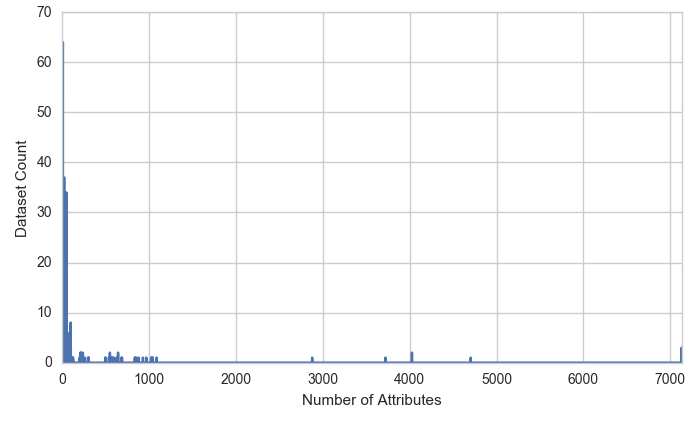
\includegraphics[width=14cm]{Images/numberOfAttributesDistribution.png}
	\centering
	\caption{Distribution of number of attributes among datasets in the OpenML dump.}
	\label{fig:numberOfAttributesDistribution}	
\end{figure}

The remaining datasets were examined for the distribution of the OpenML global metafeatures. The distribution is shown in Figure \ref{fig:globalmetadatadistirbution}. Not all global metafeatures are computed for each dataset. Luckily for us, in this case few metafeatures have useful property ensuring that if this metafeature was computed, then all others are computed (example of such metafeature was  kNN\_3NKappa). To fulfil the second criterion, it was then sufficient enough just to create a filter that one of these metafeatures cannot be null. After application of this filter, only classification datasets remained.

\begin{figure}
	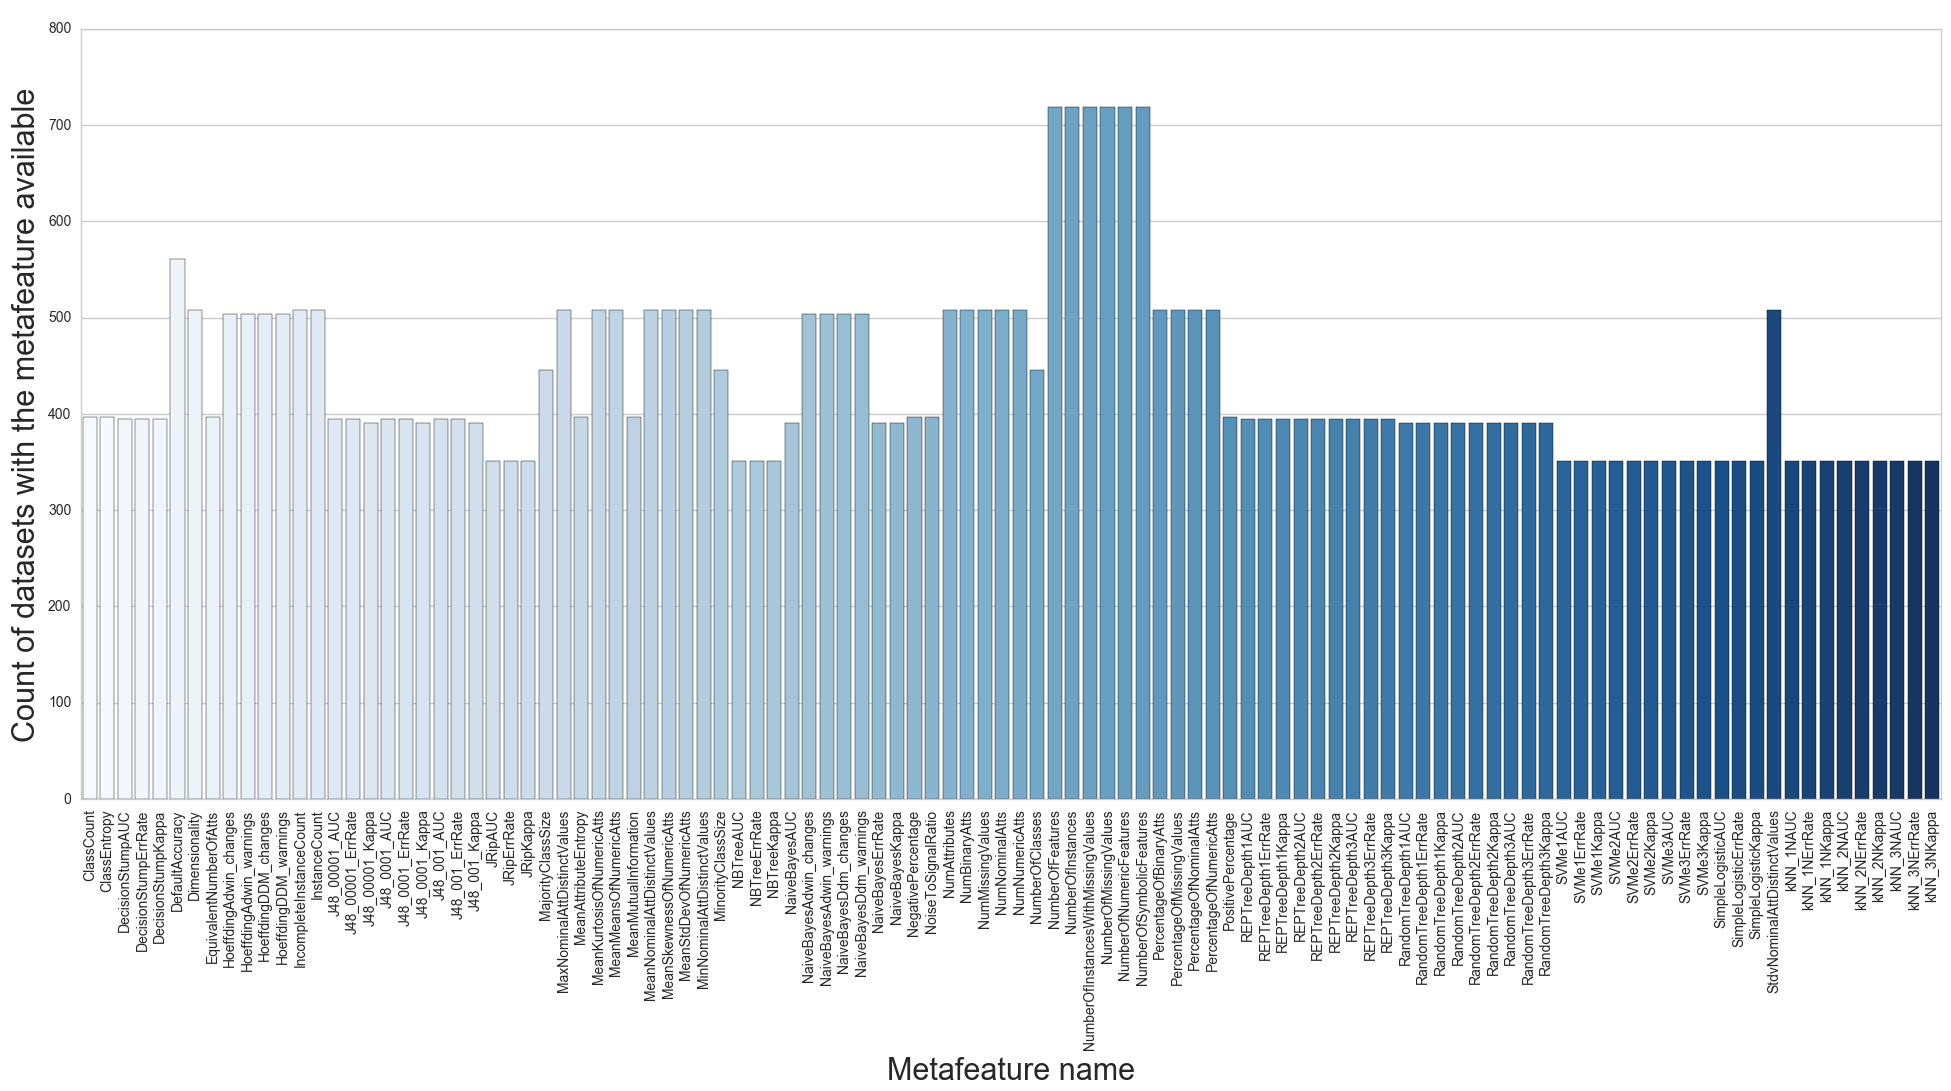
\includegraphics[width=14cm]{Images/OpenMlDataDistributtion.png}
	\centering
	\caption{Distribution of global metafeatures computed by OpenML.}
	\label{fig:globalmetadatadistirbution}	
\end{figure}

This data preprocessing included only dataset specific view. However, in our experiments the experiment results are also needed, which -- in the case of OpenML -- are covered by OpenML tasks and runs. First requirement was clear -- we can include only those datasets with the results available. Before stating another requirements, we have to choose some sort of performance criterion that will be used. We have already made the choice of restricting the datasets to classification datasets only. There are lots of performance measures possible for the classification task. When choosing a suitable measure, we wanted to include the criterion that is often used. This would minimize the filtering of datasets as this performance measure will be often available for each classification task. Based on this reasoning, we have chosen  Predictive Accuracy (see Definition \ref{definition:predictiveAccuracy}). There could still be multiple classification tasks defined with Predictive Accuracy as the performance measure -- they could still differ in the estimation procedure (simple training/testing split of the dataset, cross-validation, etc.). In order not to filter the data further, we have decided to neglect this difference, as the performance indicator is well defined regardless of the estimation procedure. Given the above, we can state the second requirement: we will include only those datasets that have some experiments results available with the Predictive Accuracy as one of the evaluation measures. 

There could be multiple results for a pair of algorithm, dataset. The question was which result to choose when arguing about the actual ranking of the algorithms on datasets. We argued that we want to asses the maximal potential of some algorithm. The best result also usually corresponds with a solution found by a hyper-parameter optimizer. Therefore, we have used the result with the best Predictive Accuracy.
 	
Finally, the results of ensemble algorithms like bagging, boosting, stacking and rotation forests \cite{rotationForests} were omitted. These ensembles are encompassing different number of other machine algorithms and can take advantage of such combined power. Such composite behaviour resulted in heavily outperforming every other algorithm in the database, thus changing the results significantly. Furthermore, their performance relies heavily on the parameters that specify what algorithms should be used in the ensemble and as such, every parameter setting should be better treated as a separate algorithm. More careful examination is thus necessary before including ensemble algorithms into our experiments.

Application of the filters resulted in 351 datasets with 20,719 rows of the best results with Predictive Accuracy for some pair of algorithm and dataset. That included 115 unique algorithms.

These amounts may seem low for machine learning experiments, but they are still much bigger that in our previous experiments, and are very high also compared to the rest of the metalearning experiments found in the literature.

Unfortunately, not every algorithm was run over every dataset. Therefore, results of some algorithms did not have to appear in the neighbourhood considered by the $k$-NN algorithm. We decided to calculate the ranking only for the algorithms that were available in the neighbourhood. This could affect the quality of ranking evaluation, however, such negative consequences can be minimized by choosing high enough $k,$ so the neighbourhood is more likely to contain more algorithms. Furthermore, high values returned by ranking quality evaluator still means high quality ranking, although not on every dataset. This can be seen as a noise or as missing values presented in the data.

The final question was splitting the data into the training and testing datasets. As the space was not very dense, and the $k$-NN that we were going to use is very dependent on the space density, we decided to split the datasets with 1:1 ratio. This enabled better estimation of the overfitting. If we used a different ratio, even the model with good generalization abilities could have much different results on the testing dataset, because of the space with much different density.

\section{Metadata}
This section will discuss which metadata were available or computed. First, we are going to discuss global data. Second, attribute metadata are described. This section also discusses normalization of both the global and attribute metadata. Note that different algorithms use different metadata, this will be elaborated when discussing experiment details.

\subsection{Global Metadata}
 As discussed in the previous section, we have filtered the OpenML dump in such a way that every metadata is available for each dataset. 
 We have argued whether we should include all the types of global metadata or just the simple, statistical, and information-theoretic ones. There are two reasons for this. First, we will base the attribute metafeatures on the simple, statistical, and information-theoretic types. Including the model based and landmarker features would make it harder to see whether the aggregation of attribute metafeatures indeed lose important information. Second reason is that model based and landmarkers metafeatures can contain information about performance on the the training and testing set. We would have to filter the training and testing set for such use to mitigate this risk. For these reasons, we have decided to use only the simple, statistical, and information-theoretic global metafeatures. In the production use, we would however include metadata of every type.
 
OpenML machine learning repository contained the following simple, statistic, and information theoretic global metadata:
\begin{itemize}
	\item ClassEntropy -- entropy of the target attribute.
	\item DefaultAccuracy -- default accuracy obtained by the baseline algorithm. In this case by predicting always the majority class. 
	\item Dimensionality -- number of attributes divided by the number of instances.
	\item InstanceCount -- number of instances (rows) of the dataset.
	\item MajorityClassSize -- number of instances with the most frequent class of the target attribute.
	\item MaxNominalAttDistinctValues -- the maximum number of distinct values among attributes of the nominal type.
	\item MinNominalAttDistinctValues -- the minimal number of distinct values among attributes of the nominal type.
	\item MinorityClassSize -- number of instances with the least frequent class of the target attribute.
	\item NumAttributes -- number of attributes (columns) of the dataset.
	\item NumBinaryAtts -- count of binary attributes.
	\item NumNominalAtts -- count of nominal attributes.
	\item NumNumericAtts --  count of categorical attributes.
	\item PercentageOfBinaryAtts -- percentage of binary attributes.
	\item PercentageOfNominalAtts -- percentage of nominal attributes.
	\item PercentageOfNumericAtts -- percentage of numerical attributes.		
	\item NumberOfClasses --  number of classes for the classification task.
	\item IncompleteInstanceCount -- number of instances with at least one value missing.
	\item NumMissingValues -- number of missing values in the dataset.
	\item PercentageOfMissingValues -- percentage of missing values.
	\item PositivePercentage -- percentage of rows with the class with the highest assigned index. In the case of binary classification this is equal to percentage of positive instances.
	\item NegativePercentage -- percentage of rows with the class with the lowest assigned index. In the case of binary classification this is equal to percentage of negative instances.	
	\item MeanAttributeEntropy -- mean of entropy among attributes.
	\item MeanKurtosisOfNumericAtts -- mean kurtosis among attributes of the numeric type.
	\item MeanMeansOfNumericAtts -- mean of means among attributes of the numeric type.
	\item MeanMutualInformation -- mean of mutual information between the nominal attributes and the target attribute.
	\item MeanNominalAttDistinctValues -- mean of number of distinct values among the attributes of the nominal type.
	\item MeanSkewnessOfNumericAtts -- mean skewness among attributes of the numeric type.
	\item MeanStdDevOfNumericAtts -- mean standard deviation of attributes of the numeric type.
	\item NoiseToSignalRatio -- ClassEntropy divided by MeanMutualInformation. Returns -1 if MeanMutualInformation is zero.
	\item EquivalentNumberOfAtts -- The difference of (MeanAttributeEntropy - MeanMutualInformation) divided by MeanMutualInformation. Returns -1 if MeanMutualInformation is zero.
	\item StdvNominalAttDistinctValues -- standard deviation of the number of distinct values among nominal attributes.
\end{itemize}

We have also identified some duplicates among the meatefatures: \\ NumberOfMissingValues as a~duplicate of NumMissingValues, ClassCount as a~duplicate of NumberOfClasses, NumberOfInstances as a~duplicate of InstanceCount, NumberOfFeatures as a~duplicate of NumAttributes, NumberOfNumericFeatures as a~duplicate of NumNumericAtts, NumberOfSymbolicFeatures as a~duplicate of NumNominalAtts and NumberOfInstancesWithMissingValues as a~duplicate of IncompleteInstanceCount metafeature. We have removed the duplicates out of a set of metafeatures used.

The last few attributes beginning with the MeanAttributeEntropy represent exactly those attributes where some important information may be lost during the aggregation, as discussed in Section \ref{section:NonpropositionalApproachToMetalearning}.

The excluded metadata (of model based or landmarker type) are listed in Table \ref{table:excludedGlobalMetadata}. We will omit their description, as they are no longer relevant.

 \begin{table} 
 	\caption{Excluded global metafeatures.}
 	\label{table:excludedGlobalMetadata}
 	\centering 
 	\renewcommand{\arraystretch}{1.3}
 	\begin{tabular}{|c| c| c|} 	
 		\hline 	 
	 	RandomTreeDepth1AUC & REPTreeDepth3AUC & J480001ErrRate \\
	 	RandomTreeDepth1ErrRate & REPTreeDepth3ErrRate & J48001ErrRate \\
	 	RandomTreeDepth1Kappa & REPTreeDepth3Kappa & JRipErrRate \\
	 	RandomTreeDepth2AUC & DecisionStumpAUC & NBTreeErrRate \\
	 	RandomTreeDepth2ErrRate & DecisionStumpErrRate & SVMe2ErrRate \\
	 	RandomTreeDepth2Kappa & DecisionStumpKappa & kNN1NErrRate \\
	 	RandomTreeDepth3AUC & SimpleLogisticAUC & NBTreeAUC \\
	 	RandomTreeDepth3ErrRate & SimpleLogisticErrRate &  kNN2NErrRate\\
	 	RandomTreeDepth3Kappa & SimpleLogisticKappa & J480001AUC \\
	    HoeffdingAdwinChanges & NaiveBayesAUC  & JRipKappa \\
	    HoeffdingAdwinWarnings & NaiveBayesErrRate & SVMe3ErrRate \\
	    HoeffdingDDMChanges & NaiveBayesKappa  & SVMe1AUC \\
	    HoeffdingDDMWarnings & SVMe1Kappa & SVMe2AUC \\
	    NaiveBayesAdwinChanges & SVMe2Kappa & SVMe3AUC \\
	    NaiveBayesAdwinWarnings & SVMe3Kappa & J48001AUC \\
	    NaiveBayesDdmChanges & kNN3NErrRate & kNN1NAUC \\
	    NaiveBayesDdmWarnings & kNN1NKappa & kNN2NAUC \\
    	REPTreeDepth1AUC & J480001Kappa &  J48001Kappa\\
    	REPTreeDepth1ErrRate & NBTreeKappa & SVMe1ErrRate \\
    	REPTreeDepth1Kappa & J4800001AUC & J4800001ErrRate \\
	    REPTreeDepth2AUC & kNN2NKappa & kNN3NAUC \\
   	    REPTreeDepth2ErrRate & JRipAUC &  J4800001Kappa\\
   	    REPTreeDepth2Kappa & kNN3NKappa & \\
 		\hline 
 	\end{tabular}
 \end{table}  

To sum up, we had 31 global metafeatures available for each dataset.

\subsection{Attribute Metadata}
There is no such public repository as OpenML that would have attribute metadata available for each dataset. Some information could be available in the header of the ARFF files (see Section \ref{section:arff}), but as already discussed, there is no guarantee that the information really corresponds to values in the data. Indeed, we have encountered datasets that were corrupted this way. Furthermore, this information is optional, thus not available in every header. Based on these facts, we decided to build our own ARFF analyser. The analyser was able to read the input ARFF file and extract various attribute metadata. In the rest of this section, we describe the attribute metafeatures extracted. As our algorithms are capable of handling type-specific attribute metadata using selectors (see Algorithm \ref{algo:combinedAlignmentHungarian}), we will list them according to the type of attribute they were extracted for.

In order to be able to compute some metafeatures for the categorical attributes, a conversion to the integers was made. Distinct number was assigned to each category. The number was chosen based on the order of appearance beginning with one.

Measures common for both the categorical and numerical metafeatures:
\begin{itemize}	
	\item ForRegression -- whether the target was of numerical type (this was not used as we have used only classification tasks).
	\item ValuesCount -- number of values.
	\item NonMissingValuesCount -- number of non missing values.
	\item MissingValuesCount -- number of missing values.
	\item Distinct -- number of distinct values (classed).
	\item AverageClassCount  -- average count of occurrences among different classes.
	\item Entropy -- entropy of the values.
	\item MostFequentClassCount -- count of the most probable class.
	\item LeastFequentClassCount  -- count of the least probable class.
	\item ModeClassCount -- mode of the number of distinct values.
	\item MedianClassCount -- median of the number of distinct values.
	\item PearsonCorrellationCoefficient -- Pearson Correlation Coeeficient of the values and the values of target attribute.
	\item SpearmanCorrelationCoefficient -- Spearman Correlation Coeeficient of the values and the values of target attribute.
	\item CovarianceWithTarget -- covariance of the values with the values of the target attribute.
\end{itemize}

Numerical metadata:
\begin{itemize}	
	\item IsUniform -- whether statistical test did not reject that the attribute values corresponds to a uniform distribution.   
	\item IntegersOnly -- whether attribute values contained only integers.    
	\item Min -- minimal value of the attribute values.
	\item Max  -- maximal value of the attribute values.
	\item Kurtosis -- kurtosis of the values.
	\item Mean -- mean of the values.
	\item Skewness -- skewness of the values.
	\item StandardDeviation -- standard deviation of the values.
	\item Variance -- variance of the values.   
	\item Mode -- mode of the values.   
	\item Median -- median of the values.  
	\item ValueRange -- difference between maximum and minimum of the values.  
	\item LowerOuterFence -- lower outer fence of the values.  
	\item HigherOuterFence -- higher outer fence of the values.  
	\item LowerQuartile  -- lower quartile.  
	\item HigherQuartile -- higher quartile of the values.   
	\item HigherConfidence -- higher confidence interval of the values.  
	\item LowerConfidence -- lower confidence interval of the values.      
	\item PositiveCount -- number of positive values.   
	\item NegativeCount -- number of negative values.   
	
\end{itemize}

Categorical metadata:

\begin{itemize}	
	\item Uniform Discrete -- result of Pearson's chi-squared test for discrete uniform distribution.
	\item $\chi^2$ Statistic  -- statistic value for the Pearson's chi-squared test.
	\item Ratio of attribute values that after sub-setting the dataset to that attribute value lead to different distribution of the target as indicated by the following statistical test:
	\begin{itemize}
		\item Kolmogorov-Smirnoff test (continuous target only),
		\item Mann-Whitney U-test (continuous target only),
		\item $\chi^2$-test (categorical target only).
	\end{itemize}
\end{itemize}

To sum up, we have extracted 15 types of attribute metadata available for both the numerical and categorical attributes, another 20 types for numerical attributes and 3 types for categorical attributes only.

\subsection{Normalization}
Our algorithms were designed with no prior distinction of the metafeatures.
Some metafeatures put on much bigger values than the others. If we used the vector of constant weights, the $p$-norm distance could yield distance mainly derived out of big valued attributes. This would mitigate the influence of the attributes with small absolute values even though those could contain important information. To be precise, some metafeatures in our database have values as high as 445694751099523.38 ($variance$ metafeature) and as low as -142020048 ($minimum$ metafeature), other metafeatures have by definition values constrained to some interval (for example (Spearman's Correlation Coefficient with the range of $\langle -1,1 \rangle$).

For this reason, we have normalized most metafeatures into the interval $\langle 0,1 \rangle$. Attributes already naturally constrained to that or similar interval (Spearman's Correlation Coefficient) were the exception. The normalization was performed regardless of whether the metafeature was global or attribute specific. We have used the $min-max$ normalization given by the following equation:

\begin{equation*}
x'_i=\frac{x_i - \min_{x \in \mathbb{X}}}{\max_{x \in \mathbb{X}}-\min_{x \in \mathbb{X}}},
\end{equation*}
where $\min_{x \in \mathbb{X}}$ and $\min_{x \in \mathbb{X}}$ are minimal and maximal values of the given metafeature $\mathbb{X}$, $x_i$ is specific value of the $i$-th metafeature before rescaling, and $x'_i$ the value of that metafeature after rescaling.

This solved the original problem, but sometimes another problem emerged. In some cases the majority of values lied in some small subinterval of $\langle 0,1 \rangle$. Even when the metafeature had been assigned with high weight, the distance on this single metafeature would still be around zero between most of the metafeature values and very high between few outliers and the rest of the values. This would neglect the usefulness of such metafeatures including one that could be expected to bring high discriminative factor into the distinguishing of attributes, such as maximum and minimum values.

The box plots after min-max normalization are plotted for categorical metafeatures in Figure \ref{fig:categoricalAttributeDistribution} and  for the numerical attributes in Figure \ref{fig:numericalAttributeDistribution}.
The metafeatures suffering from such problem are those whose boxplot is small compared to the interval. In some cases, the boxplot quartiles are blending together and such cases are the most problematic ones. 
To partially mitigate the problem, we have introduced virtual metafeatures, that means metafeatures computed given different features that were independent of the values and size of the dataset - percentage or boolean values calculated out of metafeatures. Percentage or boolean are naturally normalized between $\langle 0,1 \rangle$ and should not have some outliers as in the case of metafeatures based on counts. The virtual metafeatures added were the following:

Measures common for both the categorical and numerical metafeatures:
\begin{itemize}
	\item MissingValues -- Boolean whether count of missing values is greater than 0.
	\item AveragePercentageOfClass -- Percentage of the occurrences among classes, calculated by AverageClassCount/Values count.
	\item PercentageOfMissing -- Percentage of missing values in the attribute, calculated by MissingValuesCount/Values count.
	\item PercentageOfNonMissing -- Percentage of non missing values in the attribute, calculated by 1 - Percentage of missing.
	\item PercentageOfMostFrequentClass -- Percentage of the most frequent class calculated as Most Frequent Class Count/Values count. 
	\item PercentageOfLeastFrequentClass -- Percentage of the least frequent class calculated as Least Frequent Class Count/Values count. 
	\item ModeClassPercentage -- Percentage of mode of class count calculated as Mode Frequent Class Count / Values count.
	\item MedianClassPercentage -- Percentage of median of class count calculated as Median Frequent Class Count / Values count.	
\end{itemize}

Numerical metafeatures:
\begin{itemize}
	\item PositivePercentage -- Percentage of positive values calculated as $\frac{PositiveCount}{ValuesCount}$.
	\item NegativePercentage -- Percentage of negative values calculated as $\frac{NegativeCount}{ValuesCount}$.  
	\item HasPositiveValues -- Boolean whether attribute values contain positive values. Determined as the result of $PositiveCount > 0$.
	\item HasNegativeValues -- Boolean whether attribute values contain negative values. Determined as the result of $NegativeCount > 0$.
\end{itemize}

Adding the virtual attributes does not mean that the rest of the problematic features should be thrown away. They could still be valuable for detecting outliers in the data, thus useful for identifying distant attributes (or datasets).

In total we have added 8 virtual metafeatures available regardless of attribute type and 4 virtual attributes for the numerical attributes. With the number of original attributes, it made 23 attributes for all types, 24 for numerical attributes, and additional 3 for categorical attributes.

\begin{figure}
	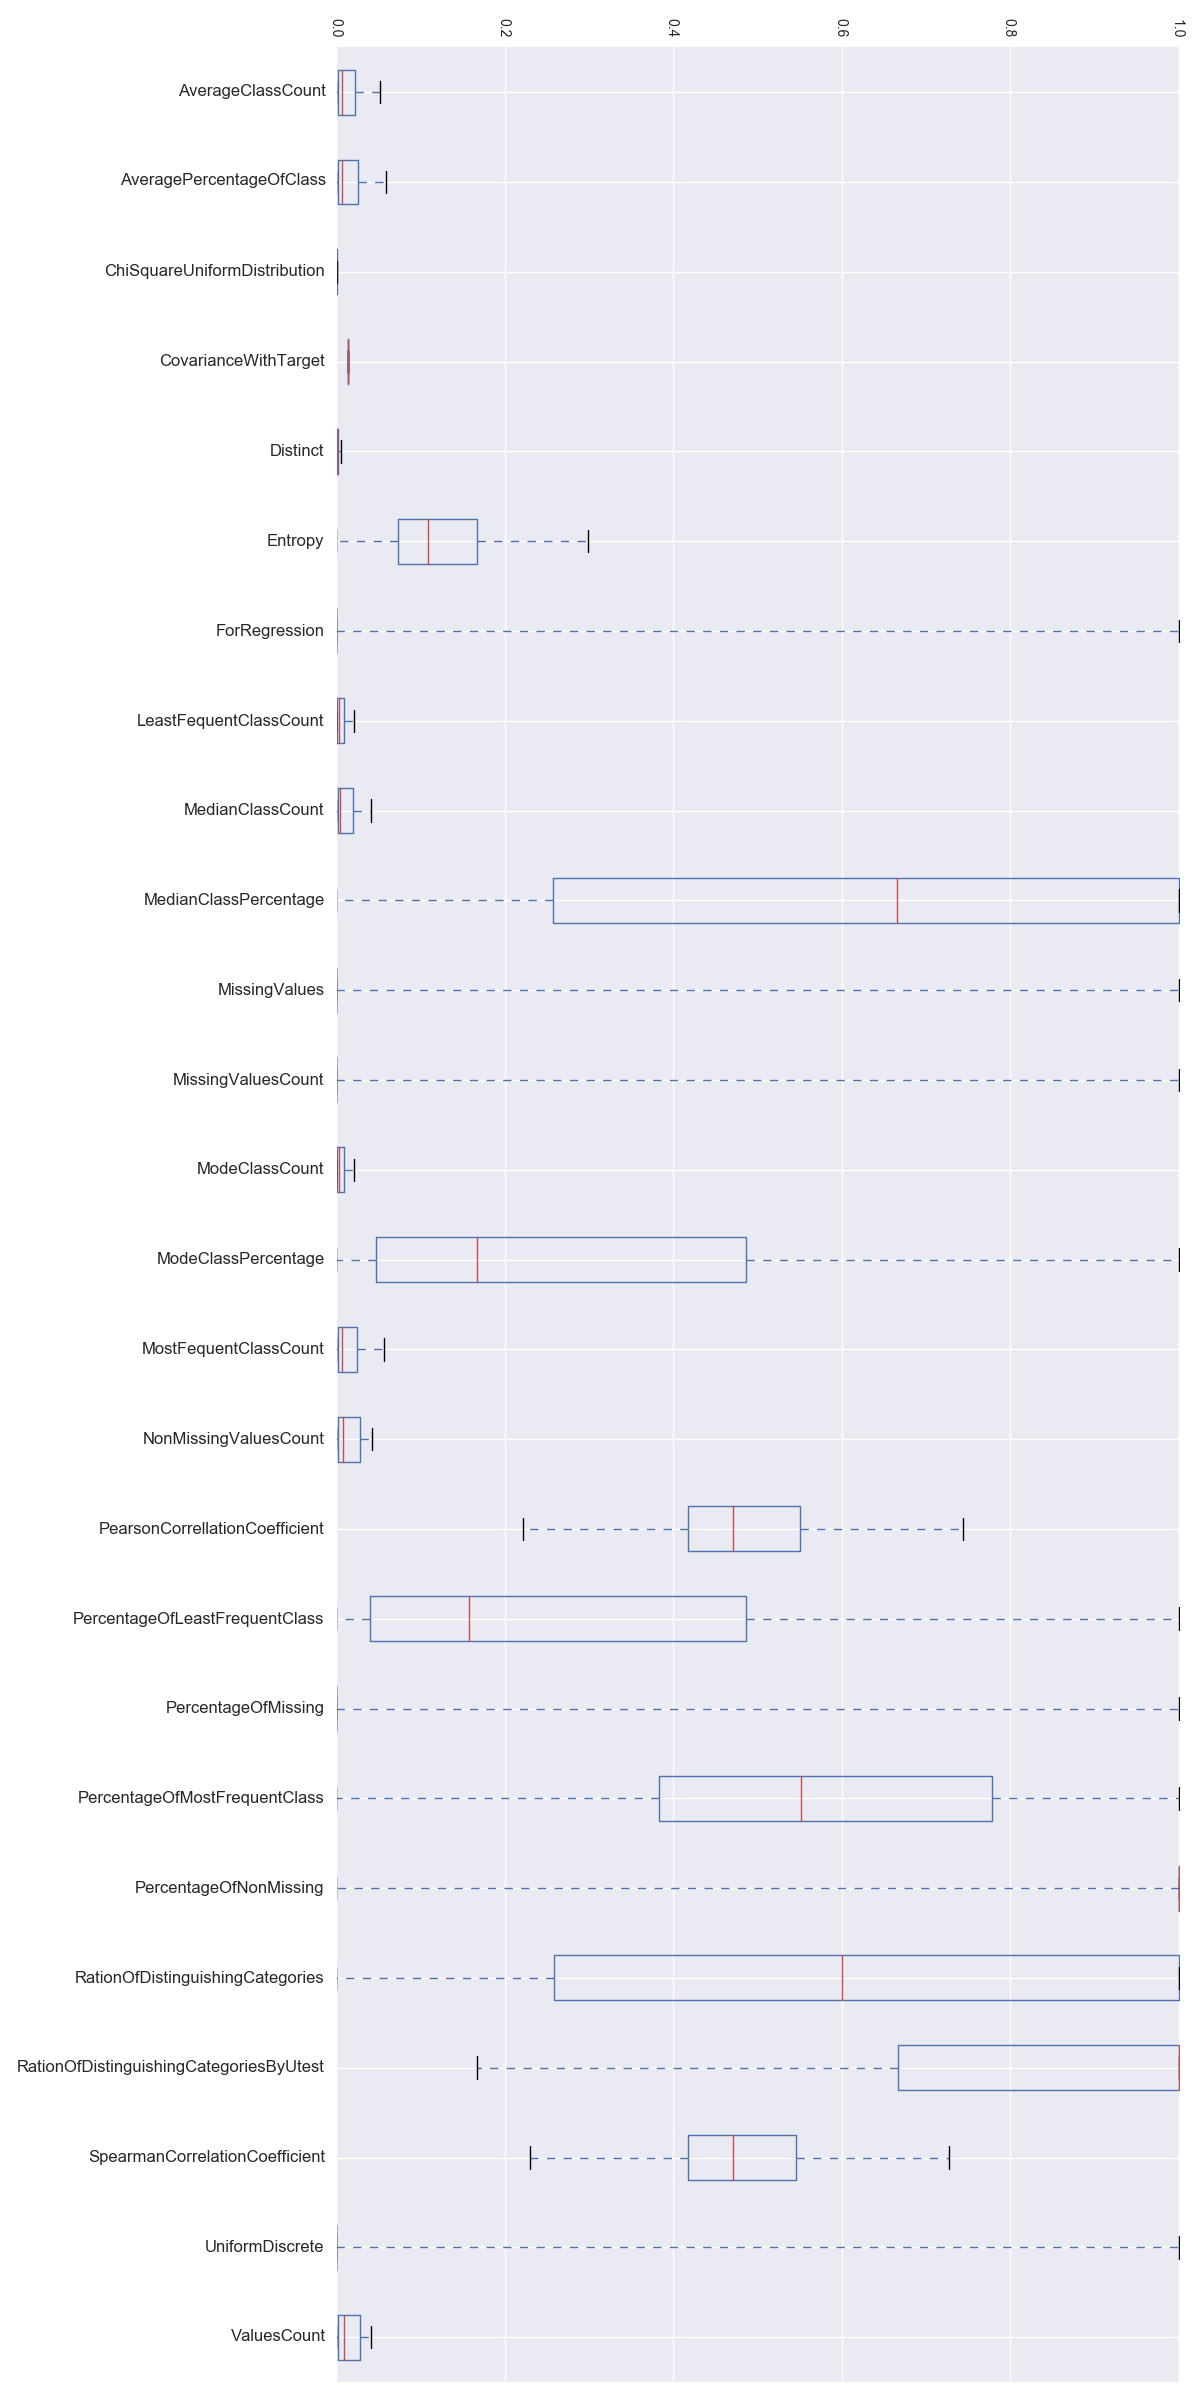
\includegraphics[width=12cm]{Images/categoricalAttributeDistribution.png}
	\centering
	\caption{Distribution of values of categorical metafeatures after normalization.}
	\label{fig:categoricalAttributeDistribution}	
\end{figure}

\begin{figure}
	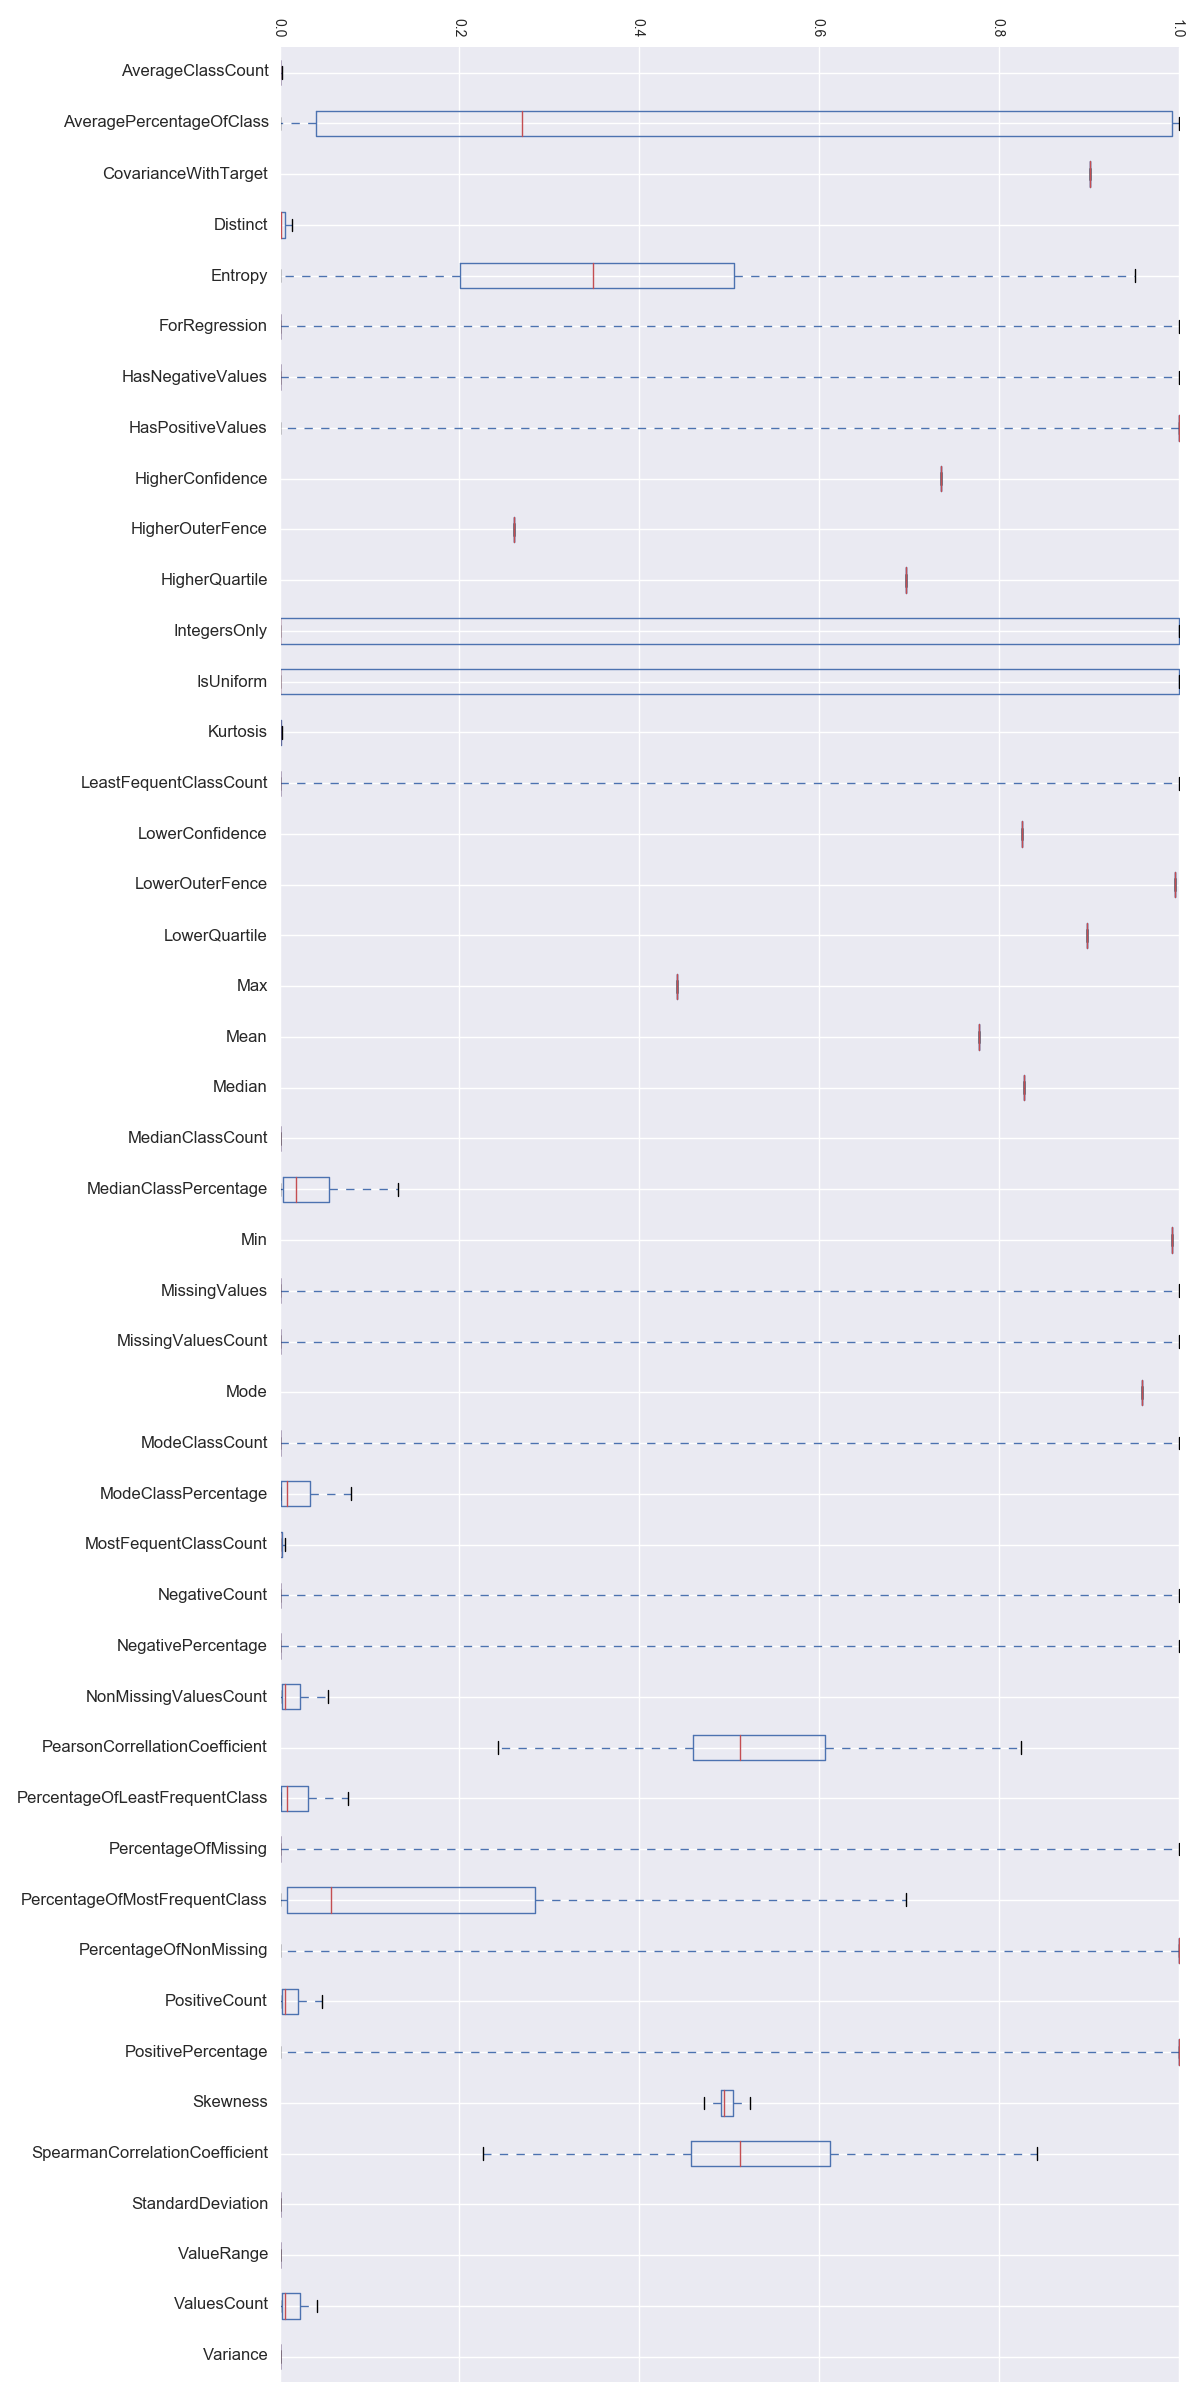
\includegraphics[width=12cm]{Images/numericalAttributeDistribution.png}
	\centering
	\caption{Distribution of values of numerical metafeatures after normalization.}
	\label{fig:numericalAttributeDistribution}	
\end{figure}
 

 
% Experiments
\chapter{Experiment Proposal}
\label{chapter:metricExperiments}
In the previous chapters, we have discussed algorithms related to the algorithm ranking problem. We are able to rank algorithms based on distance and evaluate the quality of such ranking. As was discussed in Sections \ref{section:distanceBasedRanking} and \ref{section:rankingQuality}, we can easily plug distance based ranking into the quality evaluator. The remaining argument missing is to provide $IDatasetDistance$ interface. We have discussed several algorithms being able to conform to this interface. Some of these algorithms need extra information as an input -- weights. This enables us to optimize the weights in order to maximize the quality of ranking.
We begin by defining the \emph{optimization problem} in which some space of parameters is searched in order to get the optimal solution given some evaluation criteria. We then introduce the class of optimization algorithms called \emph{Genetic Algorithms} (GAs) that are inspired by the evolution of species occurring in the nature. The general form of the algorithms is outlined and different parts are discussed -- \emph{selection}, \emph{crossover} and \emph{mutation} in more details.

We can use the GAs to optimize the weights of the algorithms for measuring the dataset distance. Metadata available was discussed in the previous chapter. 
Several experiments are proposed on the data available. Baseline, attribute alignment, and global attribute distance measure based on weighted $p$-norm with different values of $p$ explored and weights optimized by the evolution. Further, attribute assignment with the attribute distance measure  based on weighted $p$-norm with different values of $p$ tried and weights optimized by the evolution. Final experiment proposed in this section is the aggregation of the global and attribute distance measures with the importance of both counterparts also optimized. 

A big picture of all algorithms plugged together is provided. This will be possible because we have been careful in proposing algorithms in such a way that algorithms are easily pluggable to others, as they conform to the same interfaces. This overview is useful, as the number of algorithms plugged in together is large, and the whole workflow is complicated.
We also discuss the choice of all other settings of all algorithms (extending attribute space by $\dummy$ attributes, parameters for the GA, etc.)
The parameters will be chosen according to the results of Theorems \ref{theorem:metricPreservation}, \ref{theorem:dummyConstantMinimalDistance}, and \ref{theorem:metricRestoration}, so the resulting distance between datasets is a metric.
We will review the results of our experiments and discuss them. As we will see, new proposed algorithms can outperform the baseline and even improve the global attribute distance with statistical significance.

\section{Optimization}
We have provided a means of measuring the quality of distance based ranking. Some of the distances are based on weighted $p$-norms. We could try to find out such weights that result in the best ranking according to the evaluator. This is captured by the following definition:
\begin{definition}
	In the \emph{optimization problem} we have an \emph{objective function} $f$ over a domain (or search space) $A$: $f: A \rightarrow \mathbb{R}$. In the case of a \emph{minimization} problem, the solution is $x \in A$ such that $\forall y \in A: f(x) \le f(y)$. The \emph{maximization} solution is $x \in A$ such that $\forall y \in A: f(x) \ge f(y)$.
\end{definition}
In some cases, it may be hard to find the solution of the optimization problem. Some algorithms do not guarantee the optimal solution and returns its approximation instead.
\section{Genetic Algorithms}
\label{section:geneticAlgorithms}
\emph{Genetic algorithm} is a meta search heuristic based on Charles Darwin’s evolution theory \cite{Darwin} and the laws of inheritance inferred from Gregor Mendel’s inheritance theory \cite{Mendel1866}. According to the evolution theory, the following facts hold:
\begin{itemize}
	\item Every species is fertile enough that if all offspring survived to reproduce the population would grow.
	\item Despite periodic fluctuations, populations remain roughly the same size.
	\item Resources such as food are limited and are relatively stable over time.
	\item Individuals in a population vary significantly from one another, and much of this variation is inheritable.
\end{itemize}
From these assumptions, the theory infers the following:
\begin{itemize}
	\item A struggle for survival ensues.
	\item Individuals less suited to the environment are less likely to survive and less likely to reproduce; individuals more suited to the environment are more likely to survive and more likely to reproduce, and leave their inheritable traits to future generations, which produces the process of natural selection.
	\item This slowly effected process results in populations changing to adapt to their environments, and ultimately, these variations accumulate over time to form new species.
\end{itemize}
According to the inheritance theory, inherent properties of each organism are encoded in a structure called genotype. Genotype consists of genes. Each gene corresponds to some trait in organism (e.g. colour of eyes). Genotype is inferred from parents’ genotype by crossing over their genetic material. Genotype may be also altered during organism lifetime by mutation. A phenotype is the composite of an organism's observable characteristics or traits, such as its morphology, development, biochemical or physiological properties, phenology, behaviour, and products of behaviour. Relationship between genotype and phenotype is often conceptualized as follows:

\begin{equation*}
genotype + environment \rightarrow phenotype.
\end{equation*}

Genetic algorithms (GA) were described by Holland \cite{HollandGeneticAlgorithms}, who utilized principles of the evolution and inheritance theory. Given an optimization problem, GA views the solution to the problem as an individual. In the original John Holland’s work, the individual was binary encoded, but other encodings are suitable as well. The algorithm can also treat genotype equal as phenotype and the individual directly maps to the solution. In other situation, phenotype can be derived from the individual either deterministically or stochastically. Example of the former would be treating negative values of the individual as positive or encoding of the neural network, the example of the latter would be creating an individual according to the grammar described in the genotype with different rules applicable at the same time. 

A number of individuals form a population. At first, a population of individuals is created (either randomly or by using some known sub-optimal solutions). Individuals are then evaluated based on their ability to solve the problem by a function known as fitness. Individuals proceed to next generation with probability proportional to their fitness (this step is known as \emph{selection}). In each generation, new individuals are created from random parents in the current population (this step is known as \emph{crossover}) and some individuals in the current population are altered (this step is known as \emph{mutation}). New generations continue to be created until a termination criterion is satisfied (usually conditions on fitness of some individual, average fitness in population, number of generations or time elapsed since the start of the algorithm). A pseudocode of simple genetic algorithm is shown in Algorithm \ref{algo:geneticAlgorithm}.

\IncMargin{1em}
\begin{algorithm}
	\SetKwInOut{Input}{input}
	\tcp{Pseudocode of the main loop of the genetic algorithm.}
	\BlankLine
	$P_0 \leftarrow$ initialize-population()\;
	$t \leftarrow 1$\;
	\While{\upshape termination-criterion not satisfied}{
		$P_{t+1} \leftarrow$ selection$(P_t)$\;
		crossover$(P_{t+1})$\;
		mutation$(P_{t+1})$\;
		$t \leftarrow t+1$\;
	}
	\Return bestIndividual($P_t$)\;
	\caption{Genetic Algorithm}\label{algo:geneticAlgorithm}
\end{algorithm}\DecMargin{1em}

Since genetic algorithms are stochastic and do not guarantee finding an optimal solution, it could be sometimes beneficial to repeat the whole process and take the best individual from all runs.
Mutation, crossover and other steps altering the population are often generalized as genetic operators. Genetic operators will be described when applied to one or several individuals; expansion of the operators on the whole population is typically done by applying the operator on each individual or on a sample of individuals from the population.

\subsection{Selection}
Selection determines how many offspring the individuals will have in the next generation. This should be based on fitness - in general, fitter individuals should have more offspring than those less fit. Common approaches to the selection are:
\begin{itemize}
	\item \emph{Roulette selection} – let $f_k$ be a fitness of an individual $k$. Let $F_s$ be the sum of the fitness of all individuals ($F_s = \sum_{i=1}^{n}f_i$, where $n$ is the population size). For each position in the next generation, the roulette is spun. In each spin an individual is selected with probability $\cfrac{f_k}{F_s}$.
	\item \emph{Scaling} – same as the roulette selection, except that fitness is scaled at the beginning. The most common scaling function is linear function. This can solve some problems in case all individuals have similar fitness (more like random walk) or when there are very large fitness gaps between individuals (high pressure on selecting best individuals).
	\item \emph{Rank based} – individuals are sorted by fitness in ascending order. Probability of selection is higher with higher index in the sorted set of individuals.
	\item \emph{Tournament selection} – for each position in next generation, a tournament of $n$ individuals is held. The best individual is selected by the tournament with some fixed probability $p$. If the best individual is not selected, the second best individual is selected with probability $p$ and so on. If all previous individuals are not selected, select the worst individual from the tournament. This rescales the population and thus the evolution pressure remains constant (extraordinary good individuals does not flood entire population and even the minor differences between individuals are recognized).
\end{itemize}

Some alternations of GAs perform the selection not only among the new offspring, but also among parents. Furthermore, the best solution found so far may be lost during the process. To counter this, the best individuals are sometimes guaranteed to be inserted into the next generation. This is referred to as \emph{elitism}.

In binary coding, crossover is typically implemented as a one point crossover – two parents are selected, then one point in both parents is chosen randomly, and the parts induced by the point chosen are swapped. This creates two offspring individuals. A more general alternative is the $n$-point crossover, where more points are chosen when creating the offspring. One point crossover is illustrated in Figure \ref{fig:crossover}.

\begin{figure}
	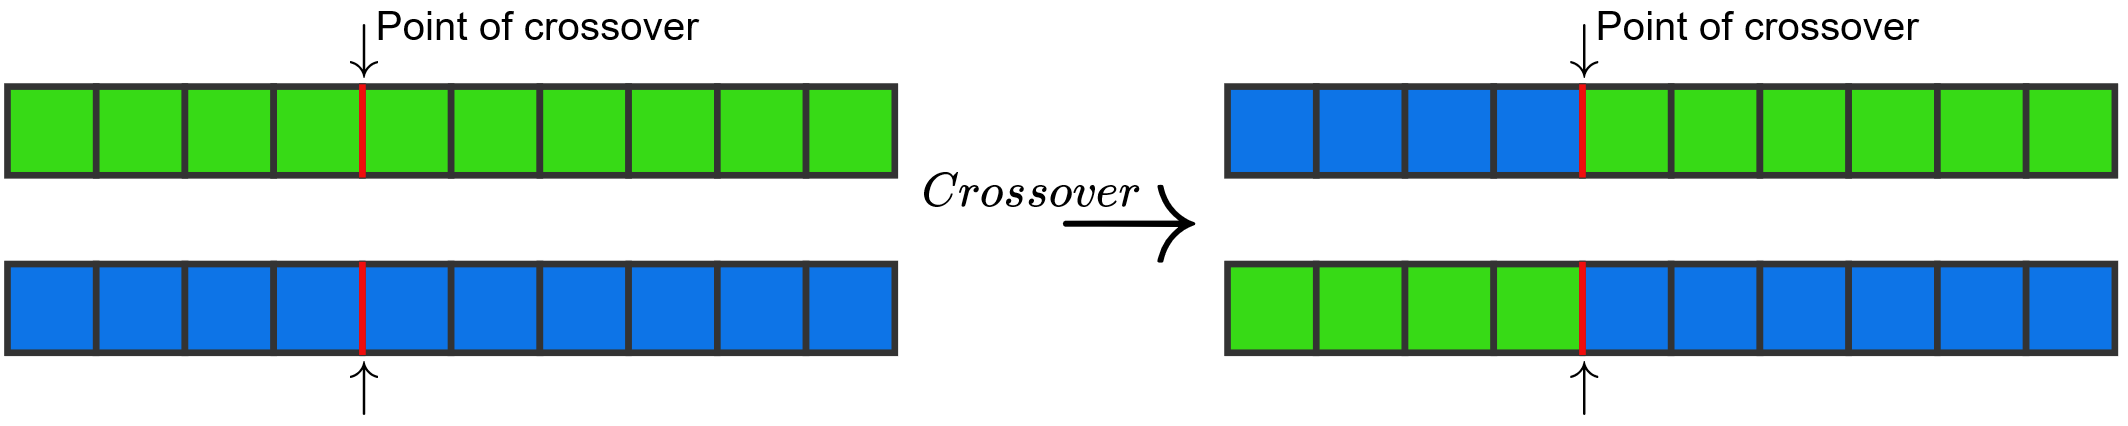
\includegraphics[width=14cm]{Images/crossover.png}
	\centering
	\caption{Example of the crossover genetic operator.}
	\label{fig:crossover}	
\end{figure}

\subsection{Mutation}
Mutation operator alters a part of an individual, thus introducing new features into population. Mutation helps explore those parts of the search space that would be otherwise hard to reach with selection and crossover only. In particular, mutation helps the genetic algorithm get out of the local optima.
In binary coding, mutation is typically implemented in a way that each bit has some small probability $p_{mutation}$ of being flipped. This is illustrated in Figure \ref{fig:mutation}.

\begin{figure}
	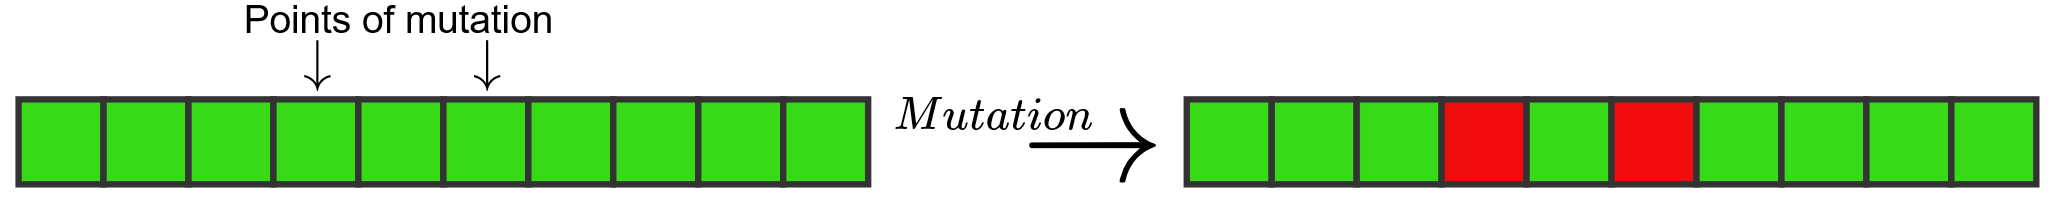
\includegraphics[width=14cm]{Images/mutation.png}
	\centering
	\caption{Example of the mutation genetic operator.}
	\label{fig:mutation}	
\end{figure}

\subsection{Modifications}
One of the advantages of genetic algorithms is their versatility. It is easy to change different parts of the algorithm to accustom for the needs.
For example if we have some knowledge about the problem we aim to solve, we may introduce operators tailored to the problem. Such operators often achieve better results than classic non-specialized operators.
Alternatively, we can create additional evolutionary pressure if the evaluation of the fitness is costly (either time or money) so the algorithm converges quickly. Other approaches include controlling the parameters, so the algorithm does not get stuck in local optima and the diversity of individuals in the population is empowered.

\section{Experiments}
\label{section:firstExperiments}
We have all the pieces we need to propose different experiments settings. We have different ranking measures, different distances measures that can be optimized, optimization algorithm, data, metadata, and we are also able to evaluate the quality of different ranking algorithms. In this chapter, we finally connect these components together.
Since we have designed the system interfaces in a versatile way, we will be able to plug in different components into algorithms, thus changing the behaviour in a certain way. This will enable us to use the same framework for evaluation although the settings used may be totally different.

When proposing the full framework for experiments, we will use the top-down approach. This is because the algorithm on the top will be either the same or will not change so often and will be providing the unified experiment framework. The experiment part will be mainly carried in the bottom of the framework where we will be trying different settings and combination. The rest of this section is dedicated to the description of our experiments.

The goal of the experiments is to find a good settings for solving the ranking problem. We will use the OpenML dump discussed in Chapter \ref{chapter:obtainingData} as the data source. The quality of settings will be verified by the Ranking Quality Assessment algorithm (Algorithm \ref{algo:rankingQualityEvaluation}). The Ranking Quality Assessment needs an implementation of $IRanking$ interface as an input. According to the discussion in Section~\ref{section:baseline}, the baseline algorithm is useful in order to verify that the extra complexity present in different models has indeed improved the ranking quality. Therefore, as the first setting to try, we will add the baseline algorithm built by Algorithm \ref{algo:rankingBaseline}. This algorithm does not need any additional information other then data, thus we are finished with this experiment branch. Different implementation of $IRanking$ interface discussed in the thesis were distance based rankings. One suitable algorithm was $k$-NN algorithm (Algorithm \ref{algo:k-nnRanking}).

 Other distance based algorithms were also discussed but we were inclined to use the simpler algorithm, as the whole framework is quite large and we did not want to add an extra layer of logic or complexity without a specific reason. The transformation of $IDistanceRanking$ to $IRanking$ is done by the $partial$ application as described in Algorithm \ref{algorithm:IDatasetRankingTransformarmation}. The $k$-NN algorithm needs, besides data, a parameter $k$ and a notion of distance between datasets, as captured by the $IDatasetDistance$ interface (Algorithm \ref{interface:IDatasetDistance}). As discussed in Section~\ref{section:openMLDump}, the size of the neighbourhood should be set high enough so it is probable that the neighbourhood will contain all algorithms. We have set the $k$ to 17 (10 percent of the training datasets).

Throughout the thesis, we have discussed many options how to implement the $IDatasetDistance$. In this chapter, our aim will be to set up all the algorithms conforming to the $IDatasetDistance$ interface so the resulting distance is a metric. We will explore the non-metric settings in the chapters to follow. In Section \ref{section:distanceUsingGlobalMetadata} we reviewed distance based on global attributes. As we have shown, any distance defined on global metafeatures based on the weighted $p$-norm is a metric. The corresponding $IDatasetDistance$ implementation was outlined in the Global Metadata Distance algorithm (Algorithm \ref{algo:globalMetadataDistance}). We will try the most common types of $p$-norms -- that is $1$-norm, $2$-norm and $\infty$-norm. We let the Genetic Algorithm optimize the weights of the $p$-norms. The settings and the genetics operators used for optimizing the weights will be discussed later. 

Other implementations of the $IDatasetDistance$ interface were proposed in Chapter \ref{chapter:attributeAssignment}. These algorithms were able to deal with the unstructured dataset space by attribute assignment. We will discuss them starting with the simpler ones. Algorithm \ref{algo:attributeAlignmentMasterThesis} needs just the mapping of attribute into a single number -- $\sigma$. We have decided to use selectors for this approach. Concrete mapping for attributes were number of categories in the case of categorical attributes and difference between maximum and minimum in the case of the numerical attributes. We could also try different attribute evaluation functions $\sigma$ but regarding the time complexity to conduct the experiments, we decided to focus computational power on more expressive languages. Furthermore, Algorithm \ref{algo:attributeAlignmentMasterThesis} is a special case of Algorithm \ref{algo:combinedAlignmentHungarian}, and it is sufficient to try the more generic version to asses the potential of attribute assignment techniques. Other attribute assignment algorithms were Attribute Assignment algorithm (Algorithm \ref{algo:attributeAlignmentHungarian}) and the more generalised version the Combined Attribute Assignment algorithm (Algorithm \ref{algo:combinedAlignmentHungarian}) that split the assignments into multiple assignments given by the selectors. 

As discussed in Section \ref{section:distanceUsingAttributes}, we found it more sensible to calculate assignments of numerical and categorical attributes separately and not to mix numerical and categorical attributes together. The latter would limit the number of metafeatures that could be used. Furthermore, we argued that the distance between a categorical and a numerical attribute should be naturally high -- possibly reached by the penalization for addition of the $\dummy$ attributes to each selector. We thus decided not to use the Attribute Assignment algorithm but rather to use its more generic version -- Algorithm \ref{algo:combinedAlignmentHungarian}. We used two selectors -- one selecting categorical attributes and the other selecting the numerical attributes (Algorithms \ref{algo:CategoricalAttributesSelector} and \ref{algo:NumericalAttributesSelector}). According to Corollary \ref{corollary:metricPreservation}, the Combined Attribute Assignment algorithm produces a metric if the attribute distance measures of corresponding selectors are metric on the attribute space. According to this, we have to define categorical and numerical attribute distance as a metric. Again, we will use the most common weighted $p$-norms -- $1$-norm, $2$-norm and $\infty$-norm.  We shall set the $p$ of the norm in the same manner and we will not try one value of $p$ for the categorical distance and a different value for the numerical distance. However, we let weights to be set independently (also, the number of metafeatures is different). We will also optimize the weight of each assignment result. Again, we will use Genetic Algorithm for the optimization with the settings discussed later. Finally, we will carry out experiments with the aggregation of global and attribute metafeatures (Algorithm \ref{algo:datasetDistanceCombination} -- Dataset Distance Aggregation). We will use Algorithms \ref{algo:globalMetadataDistance} and \ref{algo:combinedAlignmentHungarian} as sub-distances. The selectors used will be the same as in the rest of the experiments. Again, we will use the same value of $p$ for each algorithm and selector. We let GA optimize all weights occurring in the algorithm including weight of each sub-distance.

We have prepared a cluster of computers to conduct the experiments with various hardware and operating system. The system was composed of MySQL database for storing the results, local SQLite database with metadata and experiment results that were distributed together with the application. As this database was large and was needed to be retrieved before each experiment, we decided to add to the application to reduce network load with multiple runs and to allow for faster queries to the database. The experiments run on the Microsoft .Net platform using C\# programming language. This is a platform that is currently supported by Windows, although there is .Net runtime called Mono for Unix-like system that has limited capability compared to the whole framework. However, we made sure to use the part of .Net that can be run by Mono, therefore we could use all the major OS platform - Windows, Unix and Mac OS. To allow for really easy redistribution, the Docker Image \cite{docker} was created. Docker is an open-source project that automates the deployment of applications inside software containers, by providing an additional layer of abstraction and automation of operating-system-level virtualization on Linux. This means that every docker image should be deployable to every computer that has docker installed. The image also has all the requirements installed like installed shared libraries and packages. This allows for smooth running of the experiments just by running the image. The image is automatically downloaded form the docker repository after entering the run command.

Before we discuss the concrete settings for the experiments, we would like to recapitulate the complexities of the whole workflow and underlying algorithms. 

If the ranking is precomputed, the computation of ranking quality has a complexity of $\mathcal{O}(n_dn_a)$ where $n_d$ is the number of datasets and $n_a$ is the number of algorithms.
 The complexity of ranking is constant for the baseline (whereas building up the baseline function takes  $\mathcal{O}(n_dn_a + n_a\log(n_a))$ time). For the distance based ranking, the $k$-NN algorithm takes $\mathcal{O}(n_d\log(n_d)+n_a\log(n_a))$ time per dataset, provided we have a distance matrix precomputed. This results in $\mathcal{O}(n_d(n_d\log(n_d)+n_a\log(n_a)))$ steps for all datasets. We will conduct the distance computation outside to save time as discussed in Section \ref{section:distanceBasedRanking}. To compute the distance between every pair of dataset we need $\mathcal{O}(n_d^2c(\globalDistance))$, where c$(\globalDistance)$ is the cost of computing the distance $\globalDistance$ between some pair of datasets. The complexity of computing the distance $\globalDistance$ using the global metadata for some parameter $p$ is $\mathcal{O}(n_m),$ where $n_m$ is the size of the vector of global metadata. The missing complexity is computing $\globalDistance$ using the assignment techniques. The selectors we use merely check whether attribute is numerical or categorical, therefore the complexity of each selector is $\mathcal{O}(n_{att})$. 
 
 The Attribute Alignment (Algorithm \ref{algo:attributeAlignmentMasterThesis}) in our case has the complexity of $\mathcal{O}(n_{att}\log(n_{att})),$ where $n_{att}$ is the bound of number of attributes in datasets (given by the selector). This is because computing the evaluation function $\sigma$ is easy if the $\sigma$ represents number of categories or difference between maximum and minimum. The complexity of Attribute Assignment with selectors (Algorithm \ref{algo:combinedAlignmentHungarian}) is $\mathcal{O}(c(\attributeDistance)n_{att}^2+ n_{att}^3)$, where $c(\attributeDistance)$ is the cost of attribute distance function. In our case the $c(\attributeDistance)$ is $\mathcal{O}(n_{att\_met})$ -- the size of the vector of attribute metadata. The $c(\attributeDistance)n_{att}^2$ part is for computing the distance matrix between two sets of attributes and the rest is for the Hungarian method. Finally, the complexity of Dataset Distance Aggregation (Algorithm \ref{algo:datasetDistanceCombination}) is the sum of complexities of individual sub-distances.
 
 The exact values of different variables influencing the complexities are shown in Table \ref{table:complexityVariablesValues}. 
 \begin{table}[htbp]
 	\caption{Values of variables influencing the complexity given by the training data.}
 	\label{table:complexityVariablesValues}
 	\centering
 	\begin{tabular}{ |c | c | c | }
 		\hline
 		Variable & Description & Value \\
 		\hline                       
 		$n_d$ & Number of attributes &  170\\
 		$n_a$ & Number of algorithms &  115 \\
 		$n_m$ & Number of global metafeatures &  31 \\
 		$n_{att}$ & Bound of number of attributes& 50   \\
 		$n_{att\_met}$ & Number of attribute metafeatures & 47    \\
 		\hline  
 	\end{tabular}
 \end{table} 
 
 The total complexity for the whole workflow for different setups of the ranking algorithms are in Table \ref{table:totalComplexities}.
 
 \begin{table} 
 	\caption{Total complexity of the whole workflow for ranking quality evaluation for different ranking algorithms.}
 	\label{table:totalComplexities}
 	\centering 
 	\renewcommand{\arraystretch}{1.3}
 	\begin{tabular}{|c| c| c|}
 		\hline %inserts horizontal line
 		Algorithm & Total Complexity (in $\mathcal{O}$) & Optimizing \\
 		\hline 
 		Baseline & $n_dn_a + n_dn_a + n_a\log(n_a)$ & No\\ 
 		\hline 
 		Attribute Alignment& $\begin{array} {r@{}l@{}} & {} n_dn_a + n_d(n_d\log(n_d)+n_a\log(n_a)) \\ & {} + n_d^2n_{att}\log(n_{att}) \end{array}$ & No\\    \hline 
	 	Global Distance& $\begin{array} {r@{}l@{}} & {} n_dn_a + n_d(n_d\log(n_d)+n_a\log(n_a)) \\ & {} + n_d^2n_m \end{array}$ & Yes\\    \hline 
 		Attribute Assignment& $\begin{array} {r@{}l@{}} & {} n_dn_a + n_d(n_d\log(n_d)+n_a\log(n_a)) \\ & {} + n_d^2(n_{att\_met}n_{att}^2+n_{att}^3) \end{array}$ & Yes\\    \hline 
 		Aggregation& $\begin{array} {r@{}l@{}} & {} n_dn_a + n_d(n_d\log(n_d)+n_a\log(n_a)) \\ & {} +  n_d^2(n_{att\_met}n_{att}^2+n_{att}^3+n_m) \end{array}$ & Yes\\    \hline 
 	\end{tabular}
 \end{table}
 
 
 
When optimizing the weights of either attribute distance or dataset distance, the complexity provided is the complexity to evaluate one individual. It is interesting that given one weight, we have to evaluate the weighted $p$-norm $\mathcal{O}(n_d^2(n_{att}^2)$ times to build up a distance matrix. As the weights are all that compose the individual in this case, we can look at our task as a reinforcement learning task, as we get a feedback from environment after $\mathcal{O}(n_d^2(n_{att\_met}n_{att}^2))$ steps.

Apparently, workflows including attribute assignments are the most costly ones. Just expression $n_d^2(n_{att\_met}n_{att}^2+n_{att}^3)$ in our case is equal to $170^2(47+50^2+50^3) \approx 2*170^250^3=7,225,000, 000$. Note that this is not the exact amount of steps taken as the expression is in $\mathcal{O}$, it merely gives the idea about the complexity of the workflow for our data. 
It takes up to three days to compute the ranking quality of the Attribute Assignment algorithm optimized by evolution with 100 individuals and 100 generations on the Intel I7 computer with sufficient amount of memory. This was a value that had to be taken into account when proposing the settings for assignment algorithms.

In algorithms with attribute assignments, the decision about how to extend attribute space with $\dummy$ has to me made. We did not want to penalize too heavily for having different number of attributes. As we want to have a metric and such small penalization is not possible for artificial $\dummyoutside$ attributes by Theorem \ref{theorem:dummyConstantMinimalDistance}, we decided to use $\dummyinside$ attribute from the attribute space. Based on the same argument with small penalizations, we created $\dummyinside$ attribute that has the value of every metafeature equal to the median value of all values of that metafeature in both the training and testing set.

The settings for the evolution was set according to our previous experiments and few short preliminary experiments we performed to estimate good values. We were not able to tune the parameters because of the computation times mentioned above. We decided to use tournament selection with elitism to preserve the best values. The tournament probability of better individual winning was set to 60 percent and the tournament size was set to three. This was to discourage earlier convergence and to boost the generalization ability. We have used crossover with the probability of 75 percent and the mutation with the probability of 10 percent. Population size was set to 100 in order to have reasonably big population and still be able to finish the computation in reasonable time. The number of generation was set as a termination criterion. The exact value was set to 70. This was again chosen based on the time of computation, while allowing for some sufficient amount of evolution cycles to evolve interesting properties. Furthermore, we did not want to have too many generations so the algorithm does not have a big opportunity to overfit the found solutions. The weights were randomly initialized out of $\langle 0,1 \rangle$ uniform distribution. However some operators could push the weight values outside of this interval -- even to zero or negative values. According to Theorem \ref{theorem:weightedpnormisnorm}, the weights must be strictly positive to have a metric. Therefore we use genotype to phenotype mapping by using the absolute value of the weights. We still allow weights to be zero. This would break the coincidence metric axiom but we rather interpret it as the algorithm decided that the corresponding metafeature is a noise, and therefore the attribute space should not contain this metafeature.

\begin{figure}	
	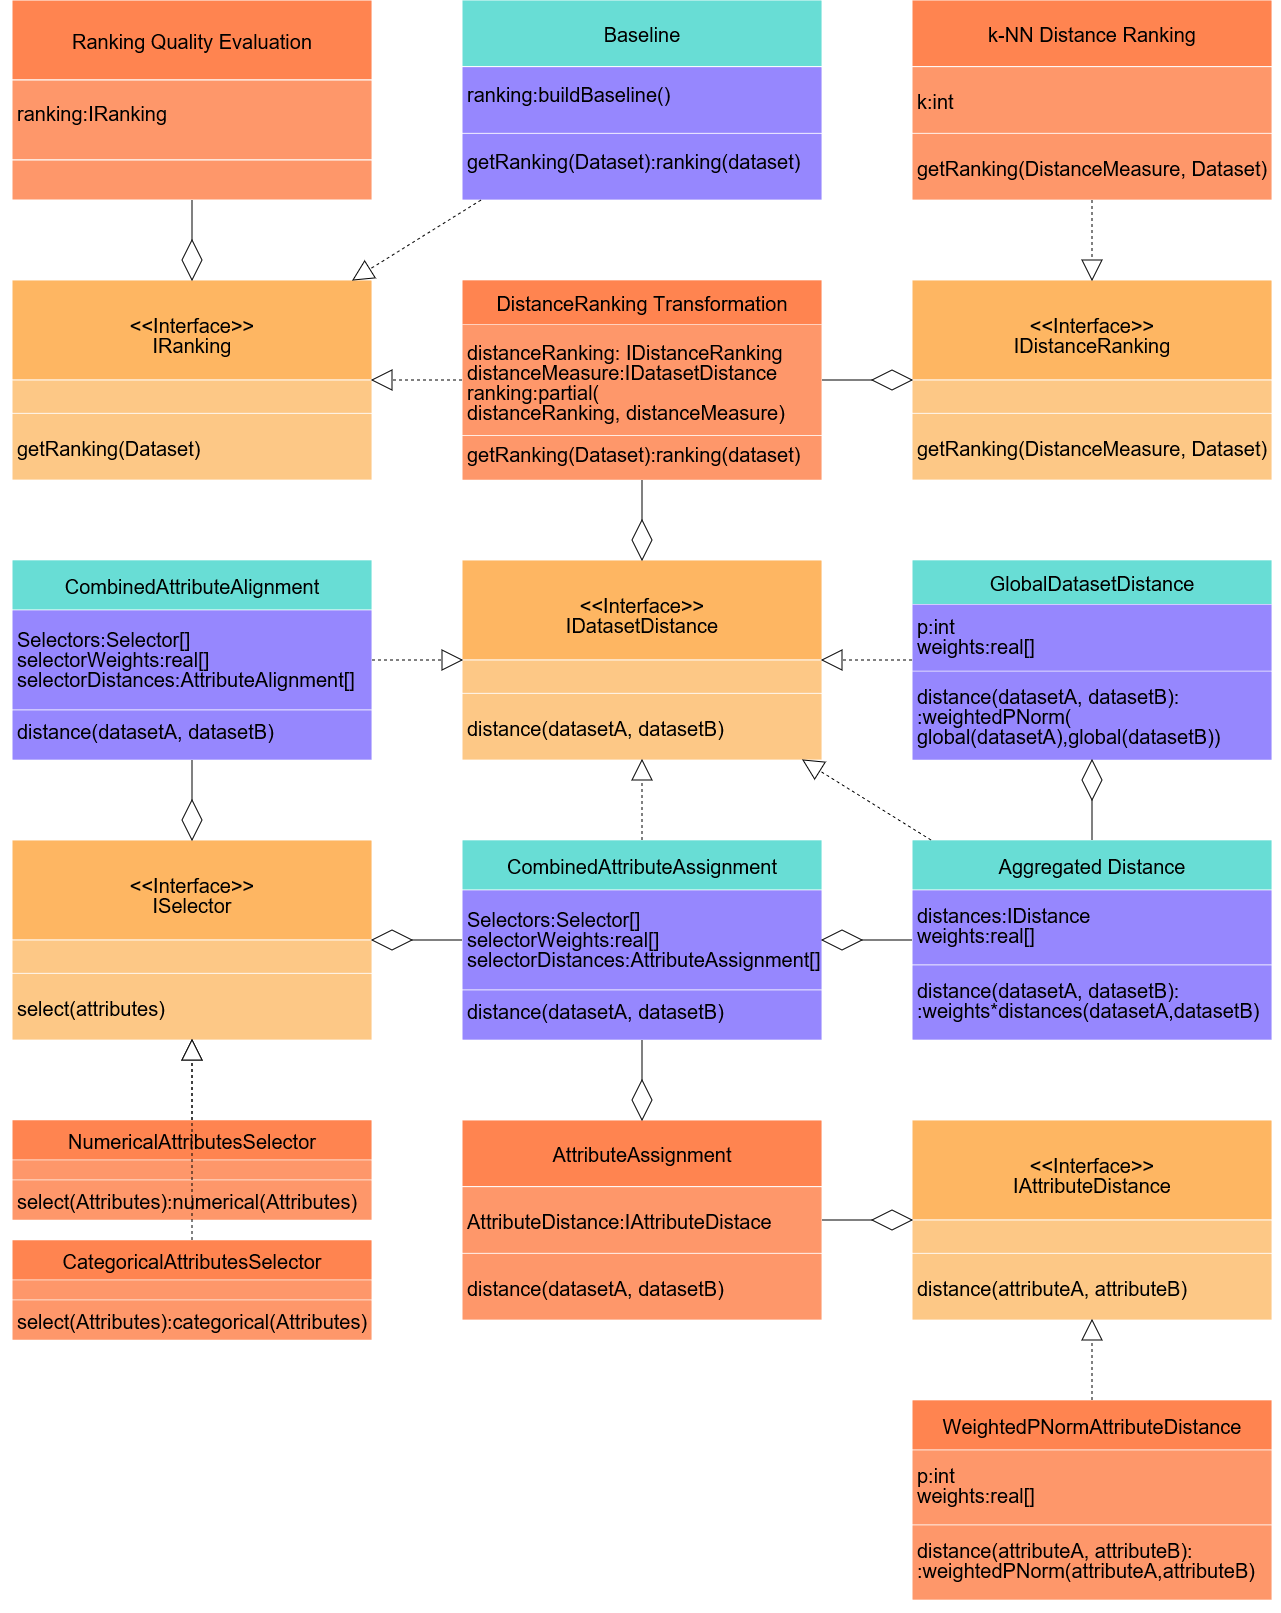
\includegraphics[width=15cm]{Images/BigPictureMetrics.png}
	\centering
	\caption{UML diagram of the whole workflow. Violet rectangles represent different ranking algorithms that will be tried in the experiments. Global Dataset Distance, Combined Attribute Assignment and Dataset Distance Aggregation will have their weights optimized by the genetic algorithm. The fitness will be provided by the Ranking Quality Evaluation. }	
	\label{fig:BigPictureMetrics}	
\end{figure}

\subsection{Results}
The results of experiments proposed in this chapter are described in the following paragraphs. Our framework uses Algorithm \ref{algo:rankingQualityEvaluation} to measure average Spearman's rank correlation coefficient (Equation \ref{eq:averageSpearman}) on the training and testing data. The higher value the better, whereas value 1 is a theoretical maximum, value -1 is a theoretical minimum, and value 0 is as good as a random guessing.

The baseline scored 0.551659 on the training set and 0.540807 on the testing set. Attribute Alignment algorithm had both testing and training score below 0.5. We believe this was because we did not optimize this algorithm. We will not discuss this algorithm further, as it is a special version of the Attribute Assignment algorithm.

The raw results of all metric-producing experiments on the testing set can be seen in Table \ref{table:metricResults}. As the runs did not have any order by definition, we sorted the values so that the first run of every algorithm corresponds to the best result of that algorithm and so on.

\begin{table}[ht]		
	\centering
	\caption{Evaluation of ranking quality of metric algorithms on the testing dataset.}
	\label{table:metricResults}	
	\begin{tabular}{cllll}

		\toprule
		\multirow{2}{*}{Run} & \multicolumn{3}{c}{ $p = 1$} \\
		\cmidrule{2-4} & Global & Assignment & Aggregation \\
		\midrule		
		1 & 0.556977 & 0.5495 & 0.563649 \\
		2 & 0.556756 & 0.54561 & 0.563345 \\
		3 & 0.556341 & 0.545248 & 0.563046 \\ 
		4 & 0.556282 & 0.543699 & 0.56146 \\
		5 & 0.555896 & 0.542449 & 0.560571\\
		6 & 0.55554 & 0.540697 & 0.559257\\
		7 & 0.555343 & 0.540422 & 0.558868\\
		8 & 0.555299 & 0.540328 & 0.558767\\
		9 & 0.555105 & 0.54024 & 0.556617\\
		10 &  0.554622 & 0.53886 &	0.556128\\
		Median & 0.555718 & 0.541573 & 0.559914 \\
		\midrule
		\multirow{2}{*}{Run} & \multicolumn{3}{c}{ $p=2$} \\
		\cmidrule{2-4} & Global & Assignment & Aggregation \\
		\midrule
			1 & 0.554876 & 0.553777 & 0.563032	\\
			2 & 0.554851 & 0.547558 & 0.560352 \\
			3 & 0.554324 & 0.547426 & 0.560273 \\ 
			4 & 0.554175 & 0.547255 & 0.558913\\
			5 & 0.554089 & 0.54587 & 0.55852\\
			6 & 0.553832 & 0.544282 & 0.557389\\
			7 & 0.553628 & 0.543237 & 0.556919\\
			8 & 0.553458 & 0.543211 & 0.556625\\
			9 & 0.553423 & 0.542909 & 0.556509\\
			10 & 0.553093 & 0.542443 & 0.554418\\
			Median &0.553961 & 0.545076 & 0.557955 \\
			\midrule
			\multirow{2}{*}{Run} & \multicolumn{3}{c}{ $p=\infty$} \\
			\cmidrule{2-4} & Global & Assignment & Aggregation \\
			\midrule
			1 & 0.557636 & 0.549426 & 0.560815	 \\
			2 &	0.55736 & 0.546354 & 0.560662 \\
			3 &	0.557084 & 0.544777 & 0.556537 \\ 
			4 &	0.557026 & 0.544307 & 0.552372 \\
			5 &	0.556069 & 0.543048 & 0.551713 \\
			6 &	0.55585 & 0.542675 & 0.551215 \\
			7 &	0.555551 & 0.541701 & 0.55055 \\
			8 &	0.555429 & 0.540912 & 0.550265 \\
			9 &	0.555058 & 0.540544 & 0.545764 \\
			10& 0.554629 & 0.537932 & 0.545444 \\
			Median &0.555959 & 0.542861 & 0.551464 \\
		\bottomrule
	\end{tabular}
\end{table}
From the raw results it can be seen that some algorithms are better than others. From the point of view of the median of the results, the order of algorithms is as follows (from best to worst): (Aggregation with $p=1$), (Aggregation with $p=2$), (Global with $p$=$\infty$), (Global with $p=1$), (Global with $p=2$), (Aggregation with $p=\infty$), (Assignment with $p=2$), (Assignment with $p=\infty$), (Assignment with $p=1$), baseline.
 
 To have a proper comparison, results of each algorithm on the testing set were compared based on the result of two tailed \emph{Mann-Whitney U Test} \cite{manWhitney}. This test is a non-parametric test with the null hypothesis that both samples come from the same population. The $\alpha$ statistics used was 0.05. The results of the tests are in Table \ref{table:metricComparisonStatisticalSignificance}. All algorithms except the Assignment algorithm with the $p=1$ were significantly better than the baseline. The best results had the aggregation of assignment and global metadata. There was no algorithm that would be significantly better than any of the Aggregated algorithms. On the contrary, Aggregated algorithms with $p=1$ and $p=2$ were significantly better than every other algorithm. There was no clear winner between those two. The results proof our hypothesis that algorithms based on attribute assignment produce useful results for ranking prediction. Also, our theory that the best results are probably obtainable by the aggregation of assignment and global distance is also supported by the results. Interesting observation is that the assignment with $p=1$ produces the worst results but the aggregation with the same $p$ provides the best results. Perhaps alignment with $p=1$ provide best additional information to support decision by the global metadata.
 
 \begin{table}[ht]		
 	\centering
 	\caption{Statistical comparison of different algorithms and their ranking quality results on the testing set. Row $i$ defines what algorithms had significantly worse results than algorithm $i$. N stands for no and Y for yes. }
 	\label{table:metricComparisonStatisticalSignificance}	
\begin{tabular}{r|cccccccccc}
	&
	\rot{Aggregation, $p=1$} &
	\rot{Aggregation, $p=2$} &
	\rot{Global, $p=\inf$} &
	\rot{Global, $p=1$} &
	\rot{Global, $p=2$} &
	\rot{Aggregation, $p=\infty$} &
	\rot{Assignment, $p=2$} &
	\rot{Assignment, $p=\infty$} &
	\rot{Assignment, $p=1$} &
	\rot{Baseline}

	
	\\ \hline
	Aggregation, $p=1$        &   & N & Y & Y&Y &Y &Y &Y &Y & Y  \\ 
	Aggregation, $p=2$        &   & & Y & Y& Y& Y& Y& Y&Y & Y  \\ 
	Global, $p=\infty$       &   & &  &N & Y & N & Y & Y & Y & Y  \\ 
	Global, $p=1$        &   & &  & & Y & N & Y & Y & Y & Y  \\  
	Global, $p=2$        &   & &  & &  & N & Y & Y & Y & Y  \\  
	Aggregation, $p=\infty$    &   & &  & &  & & Y & Y & Y & Y  \\  
	Assignment, $p=2$     &   & &  & & & & &N & N& Y  \\ 
	Assignment, $p=\infty$   &   & &  & & & & & & N& Y  \\ 
	Assignment, $p=1$     &   & &  & & & & & & & N  \\ 
	 \hline
\end{tabular} 
\end{table}


The best results on the testing set were produced by the aggregation of global and attribute metafeatures where the $p$ was set to 1. The evolution progress is shown together with the baseline in Figure \ref{fig:bestTrainingCombined}. We have measured evaluation score of the currently best individual only for statistics purpose and such measurement did not influence the run of the algorithm. It is however useful to see whether some overfitting occurred. As can be seen, the baseline was surpassed after the first generation on the training set and was above the testing baseline at all times. We can also see very high correlation between the improvement on the training set with the improvement on the testing set. At some points, some decrease of performance on the testing set can be seen but is compensated for in the further generations.
 
\begin{figure}	
	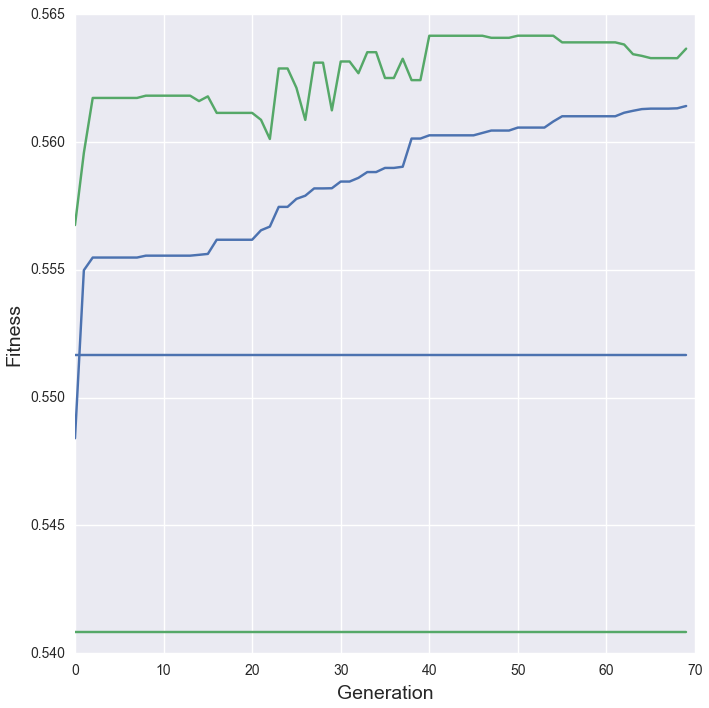
\includegraphics[width=14cm]{Images/bestTrainingCombined.png}
	\centering
	\caption{Evolution progress of the individual with the best result on the testing set together with the baseline. Results on the training set are blue, on the testing set are green. On the $x$-scale is the evolution progress, on the $y$-scale is the quality of ranking measured by the Spearman's correlation coefficient.}	
	\label{fig:bestTrainingCombined}	
\end{figure} 
 
 \subsection{Visualisation of the Distance}
 The visualization can be important for humans to interpret the results. This can be possible using kernel methods described in Section \ref{section:kernels}. Using kernelized PCA, we can project the space into two dimensions, which can be easily visualized. This requires inner product kernel. However, algorithms we use are producing metrics instead of kernels. There is a connection between these two concepts as metric represents dissimilarities and kernels similarities. We can transform distance to similarity by subtracting the distance from some large enough constant. This may not be an inner product kernel, however lots of kernel methods perform well enough with similarities close to inner products \cite{DistancesAndIndefiniteKernelsForTheSetsOfObjects}. Other approach is to repair the resulting similarity by one of the techniques proposed in \cite{PDKernels}. We have used kernelized PCA by taking the distance evolved during the run of aggregation of global and attribute approach with the best result on the testing set. The distance to similarity was transformed as follows:
 $$\text{similarity}(x,y)=100 - \Delta(x,y).$$
 The visualization of the training set is depicted in Figure \ref{fig:kpcaDistance}. We can see few clusters, but the space is mostly well covered. To check the plausibility of the visualization, we investigated the cluster of datasets in the top right region defined by $x$-component $> 1.3$ and $y$-component $> 0.2$. The datasets are listed in Table \ref{table:visualizationCluster} together with several selected metafeatures. Every dataset in the cluster is a binary classification tasks with very similar Default Accuracy. Therefore, the visualization seems to be plausible.
Being able to visualize the data is important, as it allows for a much easier interpretation.
 
 \begin{table}[ht]		
 	\centering
 	\caption{Datasets in one of the clusters in the visualization of the distance (Figure \ref{fig:kpcaDistance}).}
 	\label{table:visualizationCluster}	
 	\begin{tabular}{cccccc}
 		
 		\toprule
 		Name & OpenMLId & Attributes & Classes & DefaultAccuracy & Rows \\
 		\midrule		
 		fri\_c0\_250\_5 & 776 & 6  & 2  &  0.5 & 250 \\
 		fri\_c3\_250\_5 & 744 & 6  &  2 &  0.564 & 250	\\
 		no2 & 886 & 8  & 2  &  0.502 & 500 \\
 		wind & 847 & 15  & 2 &  0.532552  & 6574 \\
 		pbc & 810 & 19  & 2 &  0.550239  & 418 \\
 		analcatdata\_apnea3 & 764 & 4 & 2 & 0.535715 & 450 \\
 		\bottomrule
 	\end{tabular}
 \end{table}
 
 % \begin{definition}
% 	A real symmetric $N \times N$ matrix K is called  positive definite if its associated quadratic form is positive for any nonzero coefficient vector $c=[c_1, \dots, c_N]^T \in \mathbb{R}^N$, i.e.,
% 	\begin{equation}
% 	\sum_{i=1}^{N}\sum_{j=1}^{N}c_ic_jK_{ij}>0.
% 	\end{equation}
% \end{definition}
% 
% \begin{definition}
% 	A symmetric kernel K is called positive definite on $\Omega$ if its associated kernel matrix $K=\left(K\left(x_i, x_j\right)\right)_{i,j=1}^N$ is positive definite for any $N \in \mathbb{N}$ and for any set of distinct points $\left\lbrace x_1,...,x_N\right\rbrace \subset \Omega$. 
% \end{definition}
% More about positive definite kernels in \cite{PDKernels}.
% 
% If one has the similarity matrix of the training samples that is not positive definite one can try to repair the matrix in such a way that is a positive definite. In the previous section we have shown that it is easy to fix the measure to be symmetric. A symmetric matrix $S$ has an eigenvalue decomposition of $S=U \Lambda U^T$, where $U$ is an orthogonal matrix and $\Lambda$ is a diagonal matrix of real eigenvalues: $\Lambda=diag(\lambda_1,...,\lambda_n)$.
% Authors of \cite{SimilarityBasedClassificationConceptsAndAlgorithms} suggest several ways how to modify $\lambda$ to get positive definite $S'$. The mechanism is as follows: Given symmetric metric S, create the decomposition to $U\Lambda U^T$. Modify $\Lambda$ to $\Lambda_{mod}$ so that the inverse of the updated decomposition $S'=U\Lambda_{mod}U^T$ is positive definite.
% \subsubsection{Spectrum Clip}
% This technique enhances the spectrum by setting all negative eigenvalues to zero.
% $\Lambda_{clip}=diag(\max(0,\lambda_1),...,\max(0,\lambda_n))$
% \subsubsection{Spectrum Flip}
% Spectrum Flip amends the spectrum by flipping the sign of negative eigenvalues.
% $\Lambda_{flip}=diag(|\lambda_1|,...,|\lambda_n|)$
% \subsubsection{Spectrum Clip}
% $\lambda_{min}=|=min(0,\lambda_1, ..., \lambda_n)$ \\
% $\Lambda_{shift}=\Lambda+|\lambda_{min}|I$ \\
% Compared with spectrum clip and flip, spectrum shift only enhances all the self-similarities by the amount of $\lambda_{min}$ and
% does not change the similarity between any two different samples.
% \subsubsection{Spectrum Square}
% This technique follows an observation that for every square matrix S the product $SS^T$ is symmetric and also $SS^T\succeq 0$.
% If S is symmetric, the operation is equivalent to squaring its spectrum: 
% $\Lambda_{square}=\Lambda^2$
 
\begin{figure}	
	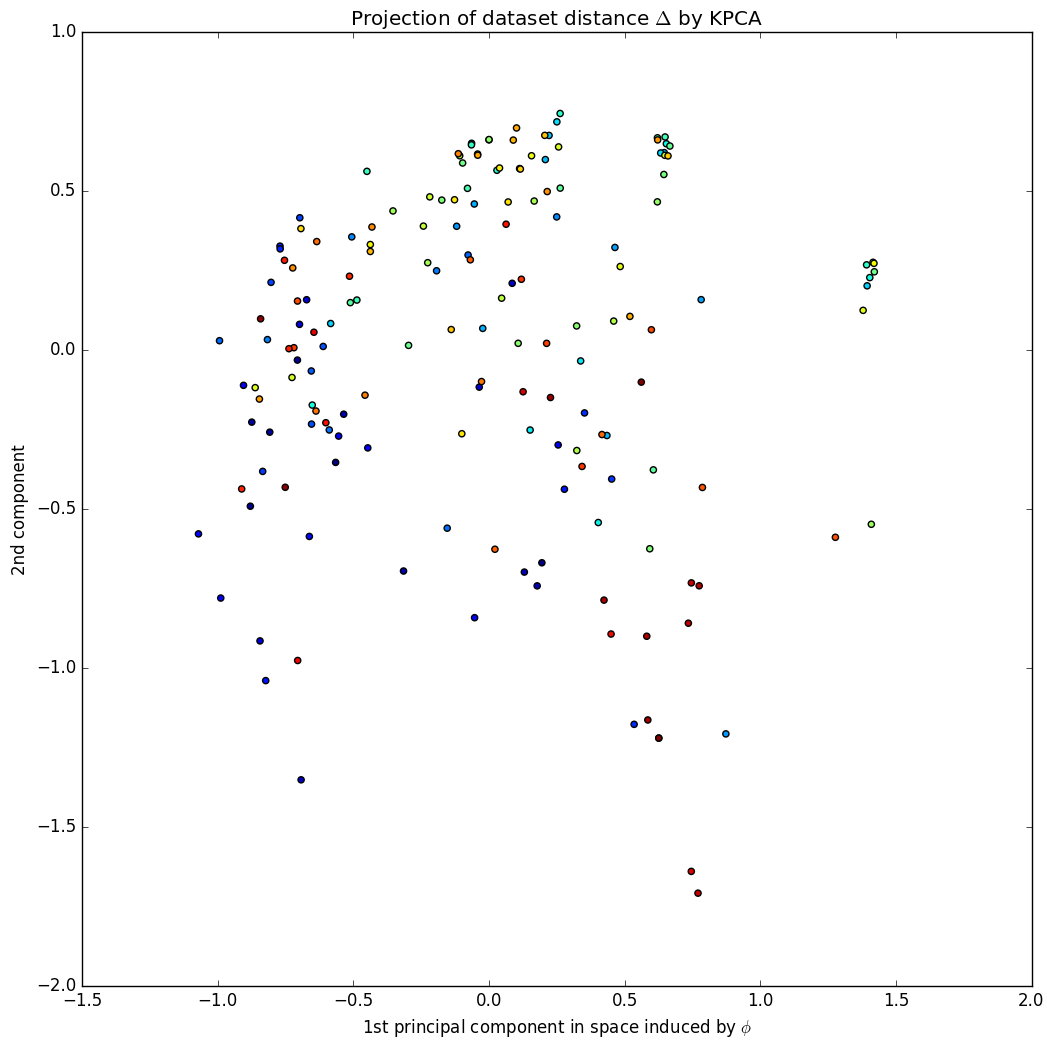
\includegraphics[width=14cm]{Images/kpcaDistance.png}
	\centering
	\caption{Projection of the training datasets using kernelized PCA and similarity based on the aggregation of global and attribute distance with the best result on the testing set.}	
	\label{fig:kpcaDistance}	
\end{figure}
 %file:///C:/Users/Jakub/OneDrive/Documents/Papers/RationalKernels.pdf
 
% GP
\chapter{Metric Relaxation}
\label{chapter:metricRelaxation}
In the previous chapters, the means of algorithm ranking have been discussed. Lots of effort has been dedicated to design algorithms that produce metrics on the dataset space induced by the attribute assignment. These algorithms were derived from the weighted $p$-norms on the attribute space. This enabled us to optimize the weights using evolutionary algorithms. We have also proven the effectivity of such approach. On the other hand, we could argue that more complex distance measure can be build on the attribute space. For instance, it seems like a good idea to enable the model to ask questions whether the attribute contain only integers or also continuous values. But instead of weighting difference of zeroes and ones, it would be perhaps a better idea to split the distance computation based on these values. For such elaborate decision, a more expressive language will be required than just a fixed-size vector of real numbers. With such added complexity we can however lose the guarantee of the attribute metric. We begin this chapter of defining relaxed versions of metrics. \emph{Semimetric} and \emph{quasimetric} are derived from metric by omitting one of the axioms -- triangle inequality and symmetry axiom respectively. We discuss which metric axioms are more important when defining a distance measure. We present a simple way of modifying arbitrary distance measure to be at least a semimetric. Then we revisit the theorems about preservations of metric from the space of attribute to the space of datasets when using attribute alignment, and we will show that the same facts hold for the preservation of semimetric. We then define a class of algorithms derived from Genetic Algorithms (see Section \ref{section:geneticAlgorithms}) called \emph{Genetic Programming} (GP). Genetic Programming, compared to the Genetic Algorithms, tries to evolve a function (or program) solving the problem instead of finding a solution to an instance of problem. Genetic Programming algorithms can be configured to produce the functions of arbitrary expression power, which will be suitable for finding more delicate attribute distance measures. We also show examples of typical GP operators. We review one of the phenomenon sometimes observable in the GP experiments -- the \emph{bloat problem}. Bloat is the tendency of some GP functions to grow in complexity, which is often accompanied by the decrease in generalization abilities of the evolved programs. In the rest of the section, we propose new batch of experiments. We discuss their expressive abilities and set their parameters in alignment with our theoretical results. We review the results of the new algorithms compared to the previous ones.

\section{Metric Spaces Revisited}
\label{section:semimetricRepairment}
In the definition of the metric (Definition \ref{definition:metric}), we have opted to use a redundant definition as the axiom 1 can be derived from the remaining axioms (Theorem \ref{theorem:metricaxiom1redundant}). This enables us however to relax the definition of the metric to introduce the terms semimetric and quasimetric:

\begin{definition}
	A \emph{semimetric} on a set $X$ is a function satisfying the first three axioms but not necessarily the fourth (triangle inequality).
	\begin{equation}
	d : X \times X \rightarrow [0,\infty),
	\end{equation}
	and for all x, y, z in X, the following conditions are satisfied:
	\begin{enumerate}
		\item $d(x,y) \geq 0$ (non-negativity).
		\item $d(x,y) = 0 \Leftrightarrow x = y$ (coincidence axiom).
		\item $d(x,y) = d(y,x)$ (symmetry).
	\end{enumerate}	
\end{definition}
\begin{definition}
	A \emph{quasimetric} on a set $X$ is a function satisfying all axioms except symmetry.
	\begin{equation}
	d : X \times X \rightarrow [0,\infty),
	\end{equation}
	and for all x, y, z in X, the following conditions are satisfied:
	\begin{enumerate}
		\item $d(x,y) \geq 0$ (non-negativity).
		\item $d(x,y) = 0 \Leftrightarrow x = y$ (coincidence axiom).
		\item $d(x,z) \leq d(x,y) + d(y,z)$ (triangle inequality).
	\end{enumerate}	
\end{definition}
In both quasimetrics and semimetrics, it is no longer possible to derive non-negativity axiom using the rest of the axioms. This is the reason why we explicitly included the first axiom into the metric definition. 

There has been a long debate in the community whether all these properties are equally important
for the similarity function in metalearning. For example, there are arguments
against the triangle inequality \cite{Ashby88towarda}, a popular example is as
follows: ``a man is similar to a centaur, the centaur is similar to a horse, but the man is completely dissimilar to the horse''. This example clearly violates the triangle inequality and speaks against using it. Moreover, it seems the coincidence axiom is also not very important. We can for example imagine, that the algorithm decides, that some of the metadata are not important for the similarity, thus returning zero even in cases where these values are different. We have addressed this by treating the attributes with the weight of zero as a noise. 
Regarding the symmetry axioms, there are some examples from the real world that are against it. For example, if we would go from place A to place B, the distance could be different from going back as we could go uphill, some paths could be blocked in one direction, etc. However, in the case of datasets, this example is not very useful because distance in the sense of dataset rather means dissimilarity than actual distance. When comparing two objects, we do not mind whether the comparison is made in a different order. Therefore, we did not consider quasimetrics further in the thesis.

Given an arbitrary distance measure $d$ on some space, we can repair the measure in such a way that it is a semimetric. For example function $d'$ defined as follows:

\begin{equation}
\label{eq:semimetricRepairment}
f(x,y) = \frac{|f'(x,y)|+|f'(y,x)|}{2}
\end{equation}
is always non-negative and symmetric. To enforce coincidence axiom, we can easily detect equal arguments on the input and return 0 otherwise. Similarly, if the $d'$ would return 0 for a non-matching input we could return some small non-negative number $\phi$ instead. Or we could return $\epsilon + d(x,y)$, for small $\epsilon > 0$. Both approaches results in semimetric, however there is a distinction. The former approach could break triangle inequality in the case $d$ was a metric. If we found three objects $k,l, z$ such that $d(k,z) < \phi/2$, $d(z, l) < \phi/2$, we could break the triangle inequality. That would happen if the $\phi$ was returned for the tuple $k,l$ instead of 0. For the triangle inequality to hold, it must be the case that the distance $\phi = d(k,l) \le d(k,z) + d(z,l)$. But at the same time, we have $d(k,z) + d(z,l)< \frac{\phi}{2} + \frac{\phi}{2}  = \phi$ from the assumptions, which is a contradiction.
We cannot do the same argument for the latter approach, as $\epsilon$ was amended to all distances of non equal objects.

\subsection{Attribute Assignment with Relaxed Attribute Measure}
In Section \ref{section:theoreticalProperties}, we have discussed how Algorithm \ref{algo:attributeAlignmentHungarian} preserves the metric properties. It turns out that Theorems \ref{theorem:metricPreservation}, \ref{theorem:metricPreservationSuportedSpaces} and Observation \ref{theorem:metricNonRestorationSupportedSpaces} are valid also for a semimetric:
\begin{corollary}
	\label{corollary:semimetricPreservation}
	Let a, b are lists of attributes, $\attributeDistance$ is a semimetric on the space of attributes $\mathbb{A}$. Then Algorithm \ref{algo:attributeAlignmentHungarian} preserves all semimetric axioms and the resulting distance $\globalDistance$ on the dataset space $\mathbb{D}$ is a semimetric.
	\begin{proof}	
	By following the proof of Theorem \ref{theorem:metricPreservation}, as the proof does not use derivation of the first metric axioms from the others (Theorem \ref{theorem:metricaxiom1redundant}), and proof of each axiom uses only the corresponding axiom on the attribute distance to prove the preservation without the use of the rest of the axioms.
	\end{proof}
\end{corollary}

\begin{corollary}
	\label{corollary:semimetricPreservationSuportedSpaces}
	Let $\mathbb{A}$ space of attributes and $A$ its subset, $\attributeDistance$ is a semimetric on $A$, $\mathbb{D}$ space of datasets. Then $\forall D \subseteq \mathbb{D}$, E supported by $A$, Algorithm \ref{algo:attributeAlignmentHungarian} preserves all semimetric axioms and resulting distance $\globalDistance$ on $\mathbb{E}$ is a semimetric.
	\begin{proof}
	By following the proof of Corollary \ref{corollary:semimetricPreservation} as the proof does not require elements outside of $D$ and $A$ and we can replace the whole $\mathbb{D}$ by $D$ and the whole $\mathbb{A}$ by $A$ respectively.	
	\end{proof}
\end{corollary}

\begin{observation}
	\label{corollary:semimetricNonRestorationSupportedSpaces}
	Let $\mathbb{A}$ be space of attributes and $\mathbb{D}$ space of datasets. Let $D$ be a subset of $\mathbb{D}$ and $\globalDistance$ a semimetric on $D$. Let $A$ be the source of $D$ and $\attributeDistance$ be a distance measure on $A$, such that Algorithm \ref{algo:attributeAlignmentHungarian} induces $\globalDistance$ using $\attributeDistance$. Then $\attributeDistance$ is not necessarily a semimetric on $A$.
	\begin{proof}
	By following the proof of Observation \ref{theorem:metricNonRestorationSupportedSpaces}, where we have shown that even though dataset distance $\globalDistance$ is a metric (thus consequently semimetric), we can define attribute distance $\attributeDistance$ to violate non-negativity.	
	\end{proof}
\end{observation}
We can draw the similar conclusions as with metric spaces. If we have a choice of optimizing between semimetric on attribute level and semimetric on dataset level, choosing the former implies optimizing the latter. This is not valid in the opposite direction.

\section{Genetic Programming}
\label{section:geneticProgramming}
To create more elaborate distance measures, more expressive language than the one used in the previous sections is required. We will also need a tool that can search in the language space and can find expressions that give a good similarity for the ranking prediction.
\emph{Genetic programming} (GP) can provide the needed functionality.

 Genetic programming is based on the same idea as genetic algorithms, where the encoding is often linear and of a fixed-length, but the search space is different. Genetic algorithms search the space of possible solutions to the problem, while genetic programming algorithms search the space of functions or programs (hopefully able to solve the problem) instead. 
 There are many ways of representing a program. Three common ways of representation used in genetic programming are \cite{FieldGuideToGeneticProgramming}:
 \begin{itemize}
 	\item \emph{Tree representation}: tree representation is traditional in genetic programming, and we will also use this representation in this thesis. Inner nodes of the tree represent operators (number of successors of the node equals arity of the operator) and leaves represent operands. Tree structures can be easily evaluated and are easy to interpret. Genetic operators are also easy to implement, as we will see later in this chapter. Usual assumption of tree representation is the property called \emph{closure} \cite{FieldGuideToGeneticProgramming}. It says that every inner node should handle arbitrary input from other operators and operands. The closure is usually obtained by using auto-conversion and/or defining operands of the same type and furthermore, every operator takes input of that type and return the output of that type. This is called type consistency. Finally, the faulty values for some operator can be handled by returning a default value for faulty input, extending the domain of that operator or decrease the fitness if the exception is thrown.
 	
 	\item \emph{Linear representation}: programs are represented as a sequence of some programming language. As we are interested in more in the actual functions taking two attribute metafeatures and not in elaborate functions taking lists or other more complex structures, Linear representation will not be considered further in this thesis.
 	
 	\item \emph{Strongly typed Genetic Programming}: proposed in \cite{typedGp}. It removes the closure requirements by defining types. This is done by introducing some restrictions into the process. We gain more freedom in defining functions. Furthermore, it can reduce the search space, as the algorithm can avoid generating some invalid input.
 	
 \end{itemize}
 The search space is determined by a language $L$ consisting of two sets – the \emph{function set} (having arity greater than zero) and the \emph{terminal set} (having zero arity). Terminals are either constants or input variables, and they occur only in the leaves of the tree representing the program. Functions are aggregating other functions and terminals, and they occur only in the inner nodes of the tree. The choice of $L$ is very important. Program solving the problem have to be encodable in this language - on the other hand, a too complex language will increase the search space exponentially, thus making finding a sufficiently good program nearly impossible. Genetic programming was used successfully in many domains. 
 
 \subsection{Initialization}
 At the beginning of the GP run, each individual in the initial population has to be randomly initialized. This can be achieved using following methods:
 
 \begin{itemize}
 	\item \emph{Full} method: This method receives an integer specifying the depth of a new individual as an input. This method creates layers sequentially. If the depth of the layer is lower than the target depth, new nodes are created by using functions, otherwise only terminals are used. This method creates a full tree of the target depth.
 	\item \emph{Grow} method: This method takes an integer specifying maximum depth as an input. New layers are created by using both functions and terminals at random. If maximum depth were to be violated, only terminals are used. By allowing terminals in the inner nodes, the distance between the root node and lists may be less than the specified maximum depth.
 	\item \emph{Ramped half-and-half}: This method creates half of the new individuals by using the full method and the other half by using the grow method.
 \end{itemize}
 
 When generating subtrees, we have to worry only about arity and generate required number of arguments. Because of the closure property we can use arbitrary inputs for every operator.
 
 \subsection{Crossover}
 The principle of the crossover operator is the same as in the original genetic algorithms.  Given two parents, one node from each parent is randomly selected. Subtrees corresponding to these nodes are swapped afterwards. This is a valid operation because of the closure property. The whole process is illustrated in Figure \ref{fig:gpcrossover}. Crossover points does not have to be selected with uniform probability. Typical GP primitive sets lead to trees with an average branching factor (the number of children of each node) of at least two, therefore  the majority of the nodes will be leaves. Consequently, the uniform selection of crossover points leads to crossover operations frequently exchanging only very small amounts of genetic material (i.e., small subtrees); many crossovers may in fact reduce to simply swapping two leaves. To counter this, authors in \cite{KozaGP} suggested the widely used approach of choosing functions 90\% of the time and leaves nodes 10\% of the time.
 
 \begin{figure}
 	\includegraphics[width=14cm]{Images/gpcrossover.png}
 	\centering
 	\caption{Example of the crossover in the Genetic Programming with the tree representation.}
 	\label{fig:gpcrossover}	
 \end{figure}
 
 \subsection{Mutation}
 Mutation alters part of the tree. A node in the parent is randomly selected. A random tree is initialized by one of the initialization method and the selected node is replaced by the new tree. Again, the closure property guarantees this to be a valid operation. The whole process is illustrated in Figure \ref{fig:gpmutation}. 
 
 \begin{figure}
 	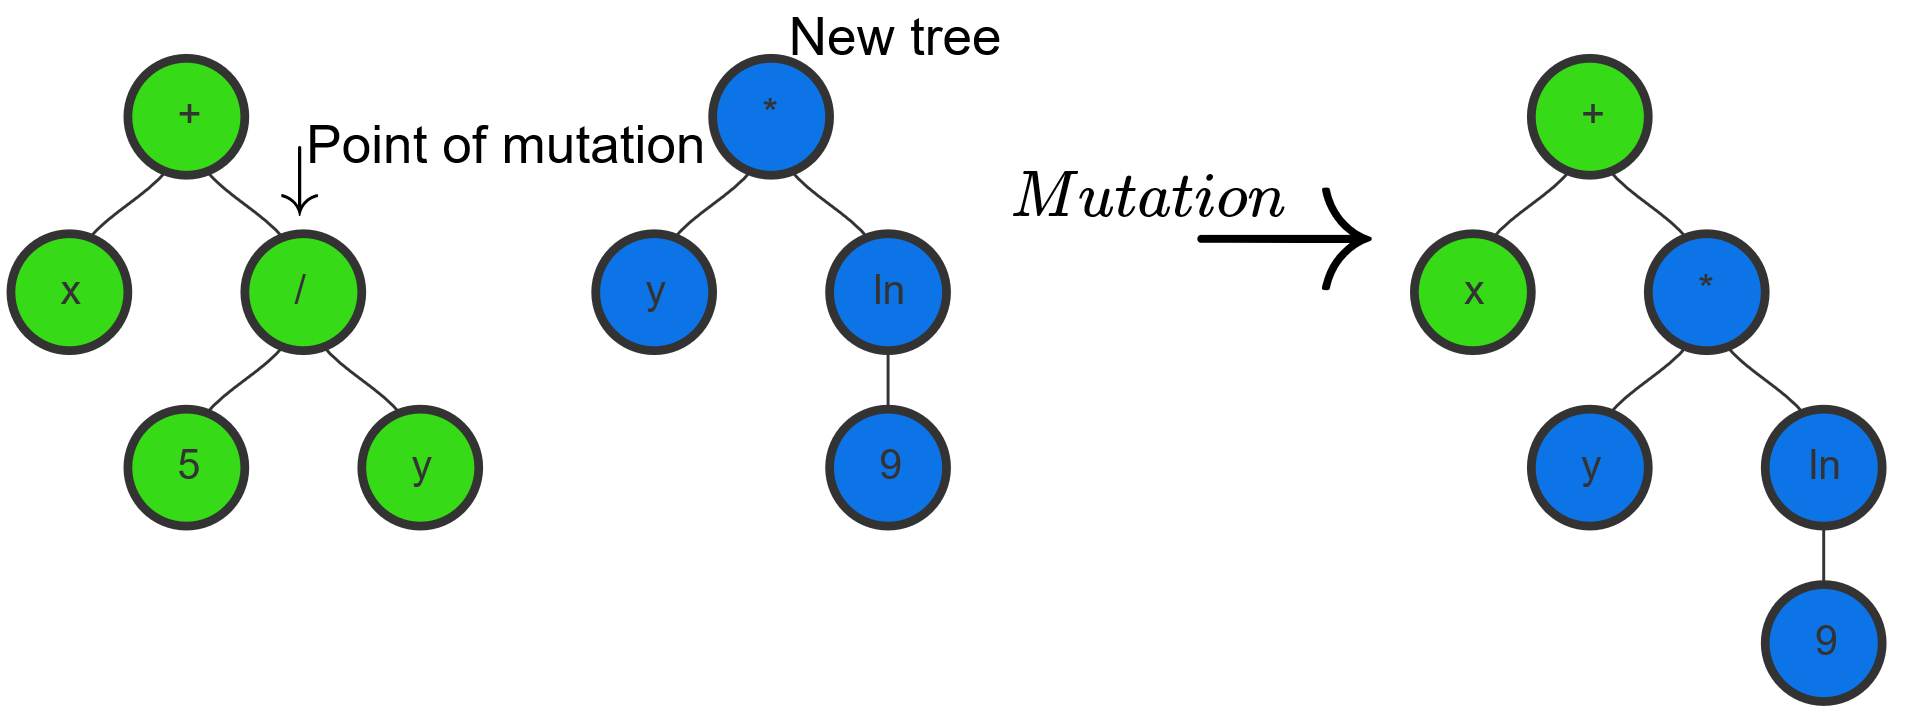
\includegraphics[width=12cm]{Images/gpmutation.png}
 	\centering
 	\caption{Example of the mutation in the Genetic Programming with the tree representation.}
 	\label{fig:gpmutation}	
 \end{figure}
 
 \subsection{Bloat Problem}
 \emph{Bloat} refers to a rapid growth of individual sizes without corresponding significant increase of fitness in later generations. In general, software bloat means that a computer program contains features that are never or rarely used. Growth alone could be beneficial, after all we are often searching complex program spaces, but without the fitness improvement it is nearly always bad. Larger individuals take more time to evaluate, take more space to store, are harder to interpret, and their ability to generalize is greatly reduced.
 There are three main theories explaining bloat \cite{FieldGuideToGeneticProgramming}:
 \begin{enumerate}
 	\item \emph{Replication accuracy theory} states that the success of a GP individual depends on its ability to have offspring that are functionally similar to the parent. As a consequence, GP evolves towards (bloated) representations that increase replication accuracy.
 	\item \emph{Removal bias theory} divides nodes in a GP tree into two categories – active code and inactive code. Inactive code is either not executed, or it is executed and its output is then discarded (for example, an inactive code would be a subtree consisting of $+(0+0+0+0)$). All remaining code is considered active. The theory observes that inactive code in a GP tree tends to be low in the tree, residing, therefore, in smaller-than-average-size subtrees. Crossover events excising inactive subtrees produce offspring with the same fitness as their parents. On average, the inserted subtree is bigger than the excised one, thus such offspring are bigger than average while retaining the fitness of their parent leading ultimately to growth in the average program size.
 	\item The \emph{nature of the program search spaces theory} predicts that above a certain size, the distribution of fitness does not vary with size. Since there are more long programs, the number of long programs of a given fitness is greater than the number of short programs of the same fitness. Over a time GP samples longer and longer programs simply because there are more of them.
 \end{enumerate}
 Techniques were designed to prevent or decrease bloat. More comprehensive survey is in \cite{LukeAntiBloatSurvey}, we will list some of the approaches:
 \begin{enumerate}
 	\item Size and depth limits. This approach checks after applying genetic operator whether the offspring is beyond the size or depth limit. If it is not, the offspring enters the population. If, instead, the offspring exceeds the limit, one of the parents is returned. Obviously, this implementation does not allow programs to grow too large. However, there is a serious problem with this way of applying size limits, or more generally, constraints to programs: parent programs that are more likely to violate a constraint will tend to be copied (unaltered) more often than programs that do not. That is, the population will tend to be filled up with programs that nearly infringe the constraint, which is typically not what is desired. The problem can be fixed by not returning parents if the offspring violates a constraint. This can be realized using two different strategies. Firstly, we can just return the oversized offspring, and assign it a fitness of 0, so that the selection will get rid of it in the next generation. Secondly, we can simply declare the genetic operation failed, and try again. This can be done in two alternative ways: a) the same parent or parents are used again, but new mutation or crossover points are randomly chosen (which can be done up to a certain number of times before giving up on those parents), or b) new parents are selected and the genetic operation is attempted again.
 	\item Anti-Bloat genetic operators. This approach modifies genetic operators to reduce the bloat. Among the bloat-control methods are size fair crossover and size fair mutation \cite{langdonSizeFairCrossover}. These work by constraining the choices made during the execution of a genetic operation so as to actively prevent growth. In size-fair crossover, for example, the crossover point in the first parent is selected randomly, as in standard crossover. Then the size of the subtree to be excised is calculated. This is used to constrain the choice of the second crossover point so as to guarantee that the subtree chosen from the second parent will not be “unfairly” big.
 	\item Anti-Bloat selection modifies the selection so that bloated individuals have lower probability to be selected into next generation. Tarpeian method \cite{PoliAntiBloatTheoreticallyMotivated} controls bloat by acting directly on the selection probabilities in the following equation:
 	\begin{equation}
 	E[\mu(t+1)-\mu(t)]=\sum_{t}l(p(l,t)-\phi(l,t)),
 	\end{equation}
 	where $E$ is the expectation operator, $\mu(t+1)$ is the mean size of the programs in the population at generation $t+1$, $l$ is the program size, $p(l,t)$ is the probability of selecting programs of size $l$ from the population in generation t and $\phi(l,t)$ is the proportion of programs of size $l$ in generation $t$. This is done by setting the fitness of randomly chosen longer-than-average programs to 0. This prevents them from being parents. By changing how frequently this is done, the anti-bloat intensity of Tarpeian control can be modulated. An advantage of the method is that the programs whose fitness is zeroed are never executed, thereby speeding up runs. Parsimony pressure method \cite{KozaGP} changes the selection probabilities by subtracting a value based on the size of each program from its fitness. Clearly, bigger programs have lower fitness and potentially less offspring under this approach. That is, the new fitness function is:
 	$f_{new}(x)  = f(x)-c l(x)$, 
 	where $l(x)$  is the size of program $x$, $f(x)$ is its original fitness and $c$ is a constant known as the parsimony coefficient.
 \end{enumerate} 
 
 \section{Experiment Proposal}
 \label{section:relaxationExperiments}
 We want to extend our whole framework with more expressive attribute distance. Again, we would like to get attribute distance in the form that can fit into our workflow. In the metric experiments we decided to use attribute alignment with selectors, as we wanted to utilize even metadata specific numerical and categorical attributes. We will do the same decision again. That gives us more specific idea for what we are looking for -- we need two functions, first computing distance between two numerical attributes and the second computing distance between two categorical attributes. In the previous section, we argued that we will use tree representation for evolved functions. To get there, we need to specify functions, terminals, make sure that we maintain the closure property, decide on the initialization and genetic operators. The main thing we need to keep in mind when proposing the whole design of the GP algorithm is that we want to generate more expressive functions. However, we will make one exception. The algorithm from Section \ref{section:firstExperiments} also evolves the weights of each selector. To evolve them using GP we would have to combine GP with GA as the vector of weights is not a tree. We decided to use the same weights for the numerical and categorical selector instead of evolving them.
 
 If not said otherwise, the proposed functions and terminals can be used regardless of the type of program evolved. All functions and terminals will be type consistent, which means that all functions will have all arguments and output of the same type. This type will be a real number in our case. If some $n$-ary function is not defined on the whole $\mathbb{R}^n$, we will propose its extended definition on the whole $\mathbb{R}^n$.
 
 \subsection{Functions}
 When discussing which function to use, we have argued that if we want to create trees with more expressive power than the previous experiments with the metric based on $p$-norms. To do that we should start by enabling the same functionality -- to add function for addition, division, square root (as we were using only $p \in \left\{1, 2, \infty  \right\}$), maximum of two values (required by the infinity norm), $p$-th power and abs. We should initialize the function set of the GP accordingly. 
 
 \begin{itemize}
 	\item Basic mathematical functions: add, subtract, multiply and divide will be used. Only division needs to be generalized. The following generalization was chosen:
 	\begin{equation*}
 	\text{Divide}(x,y)=
 	\begin{cases}
 	0; \text{ if } y = 0, \\
 	\frac{x}{y}; \text{ otherwise}.
 	\end{cases}
 	\end{equation*}
 	Based on the discussion above, we also included maximum. We decided not to include power of $p$ explicitly, as for $p=1$ or $p=2$ it can be easily evolved by the times function.
 	\item Boolean functions: normally, boolean function returns tree and false, which is usually used for branching further in the program. This would however break the closure. For the sake of type consistency, we used a trick to design Boolean functions and we proposed boolean functions (with some arity $i$) according to the following pattern:
 	\begin{equation*}
 	\text{Boolean}(a_1, \dots a_n,x,y)=
 	\begin{cases}
 	x; \text{ if } b(a_1, \dots, a_n), \\
 	y; \text{ otherwise}.
 	\end{cases}
 	\end{equation*}
 	Namely:
 	\begin{equation*}
 	\text{LessThan}(a_1,a_2,x,y)=
 	\begin{cases}
 	x; \text{ if } a_1 < a_2, \\
 	y; \text{ otherwise}.
 	\end{cases}
 	\end{equation*}
 	\begin{equation*}
 	\text{LessThanOrEqual}(a_1,a_2,x,y)=
 	\begin{cases}
 	x; \text{ if } a_1 \le a_2, \\
 	y; \text{ otherwise}.
 	\end{cases}
 	\end{equation*}
 	
 	In theory, maximum function can be obtained by these boolean functions. However, it is quite complicated to evolve as $\max(x,y)$ corresponds to $\text{LessThan}(x,y,y,x)$ and all four inputs must match. As the maximum function is quite important, we decided to add the maximum as an extra function nevertheless.
 	\item 	Other functions: we have introduced square root and base 2 logarithm. These functions were generalized by following:
 	\begin{equation*}
 	\text{SquareRoot}(x)=
 	\begin{cases}
 	\sqrt{x}; \text{ if } x \ge 0, \\
 	\sqrt{|x|}; \text{ otherwise}.
 	\end{cases}
 	\end{equation*}
 	\begin{equation*}
 	\text{Log}_2(x)=
 	\begin{cases}
 	\log_2(x); \text{ if } x \ge 0, \\
 	0; \text{ if } x = 0, \\
 	\log_2(|x|); \text{ otherwise}.
 	\end{cases}
 	\end{equation*}
 \end{itemize}
 Some other functions were also discussed:
 \begin{itemize}
 	\item Polynomial functions: We did not want to expand the domain too much, and this type of functions can be expressed by combining basic functions, so we did not introduce polynomials into population.
 	\item Periodic functions: like sin, cos. We have argued that an evolving program will not benefit from periodicity, thus we did not introduce such functions into GP domain.
 	\item Boolean functions greater than, greater than or equal. These were not introduced into the domain because they can be expressed by the means of Boolean functions already in the domain:
 	\begin{equation*}
 	\text{GreaterThan}(a_1,a_2,x,y)=\text{LessThanOrEqual}(a_2,a_1,x,y),
 	\end{equation*}
 	\begin{equation*}
 	\text{GreaterThanOrEqual}(a_1,a_2,x,y)=\text{LessThan}(a_2,a_1,x,y).
 	\end{equation*}
 \end{itemize}
 
 \subsection{Terminals}
 
 \begin{enumerate}
 	\item Constant terminals: we have proposed terminals that represent real and integer numbers. When creating such a terminal, a random number is generated and set as a value of the new terminal.
 	\item Metadata Terminals: again, we wanted to make the GP at least expressively strong enough to be able to evolve the same functions created in the previous section. In order to do this, we should cover all the attribute metadata used in the metric experiments. By the nature of metadata, some of them will be available only for the categorical trees and some for the numerical trees being evolved. Every metadata will be initialized with either one or zero. As the distance tree computes the distance function of two datasets $a$ and $b$, the zero or one will define whether the value of the terminal variable should be taken from the metadata of dataset $a$ or $b$.
 \end{enumerate}
 
 Random number terminals were also discussed. We have argued that an evolved program would not benefit from stochasticity, therefore we did not introduce such terminals into domain. Note that this is different from generating constants, because random number terminals generate a new number each time they are evaluated.
 
 The example with the individual generated for the numerical distance is in Figure \ref{fig:individualExample}.
 
 \begin{figure}
 	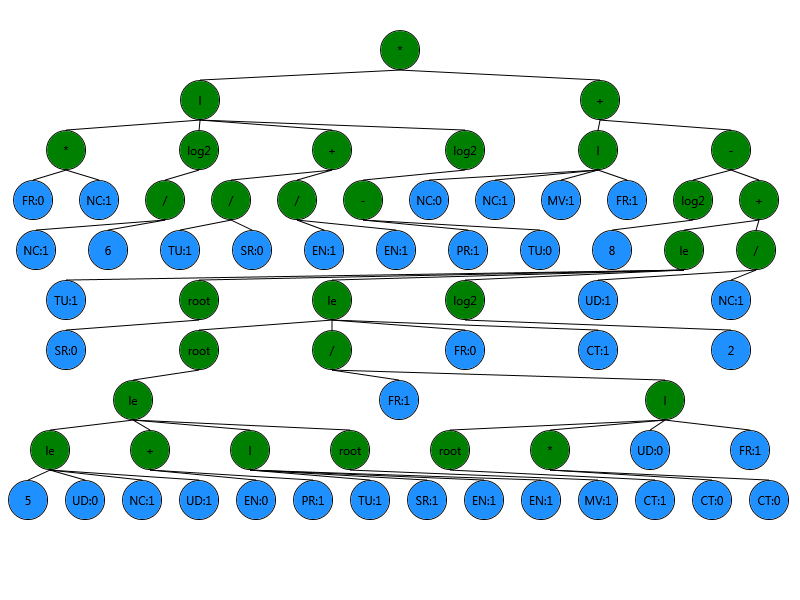
\includegraphics[width=14cm]{Images/individualExample.png}
 	\centering
 	\caption{Example of the tree evolved by the GP for the numerical distance between two attributes. The terminals are blue compared to inner-nodes which are true. The label in the node describes the type. For instance, label $l$ represents $\text{LessThan}$ function, similarly \emph{UD:0} is a variable gaining a value depending whether an attribute corresponding to the left argument (left is determined by the number 0) correspond to an uniform distribution.}
 	\label{fig:individualExample}	
 \end{figure}
 
 \subsection{Algorithm Specification}
 We need to evolve two trees. We are going to evolve these two trees as one individual. The mutation and crossover will be first applied on the categorical trees and then also on the numerical trees. As the initialization methods for the evolution, we will use the ramped half-and-half to initialize every tree. Ramped half-and-half was chosen because according to some authors \cite{FieldGuideToGeneticProgramming}, it creates more diversity. The initial maximal depth was set to 6. The mutation and crossover probabilities were set regardless of whether they are used for the categorical or numerical part of an individual. The mutation chance was set according to our previous experiments to 0.2. The probability of crossover happening was set to 0.7. The termination criterion was set to the generation count. We did not want to encourage bloating and over-fitting, so the generation target was set to 80. We believe this was the reasonable amount of generation to evolve reasonably good distance measures. Compared to the previous experiments with genetic algorithm, we also increased the population size to 120 individuals. GP is more dependent on bigger populations, as a lot of distance measures generated really bad input compared to the genetic algorithms where everything was a $p$-norm, and even the worst weights produced somewhat reasonable output.
 
 For the rest of the workflow settings, we will not make any changes. We set up number of neighbours for the $k$-NN to 17 and use the dummy attribute as the one already in the attribute space given by the median of every metafeature.
 
 Given two datasets $a$ and $b$, respectively their numerical and categorical metafeatures, the evolved tree can now compute the distance using Algorithm \ref{algo:combinedAlignmentHungarian}. This does not guarantee any of the metric properties. For instance, algorithm can produce zero easily by instantiating the minus node with two children -- each of them initiated by a constant of the same value. It would be very hard to constrain the GP algorithm to evolve only metrics or semimetrics. It would require either a limited set of functions the algorithm can use,
 or complicated operators, which would ensure these properties. Instead, based on the discussion in Section \ref{section:semimetricRepairment}, we decided to amend the values produced by the trees according to Equation \ref{eq:semimetricRepairment}, return $0$ if $x=y$ and add a small $\epsilon > 0$ if $\delta(x,y)=0$ and $x \neq y$. This will guarantee that we will have a semimetric on the attribute space.
 According to Corollary \ref{corollary:semimetricPreservation}, the resulting distance $\globalDistance$ on the dataset space is a semimetric. Thus, we sacrificed triangle inequality to gain more expressive language to describe attribute distance measures. Other option would be to repair the resulting distance between datasets. We have decided to repair the attribute distance, as aligned to the results of Corollary \ref{corollary:semimetricPreservationSuportedSpaces} and Observation \ref{corollary:semimetricNonRestorationSupportedSpaces}.
 
 The increase in the population size slightly increased the amount of time to conduct the experiments. Also, if the GP tree was deep enough, its evaluation usually took slightly more time compared to $p$-norms. This was a major factor as the function was evaluated many times. Despite this fact, we decided not to lower the number of runs so the results are easier to compare. Therefore, the number of runs was again set to 10.
 
 The whole workflow with the GP and the semimetric repairment is shown in Figure \ref{fig:BigPictureGp}.
 
 \begin{figure}
 	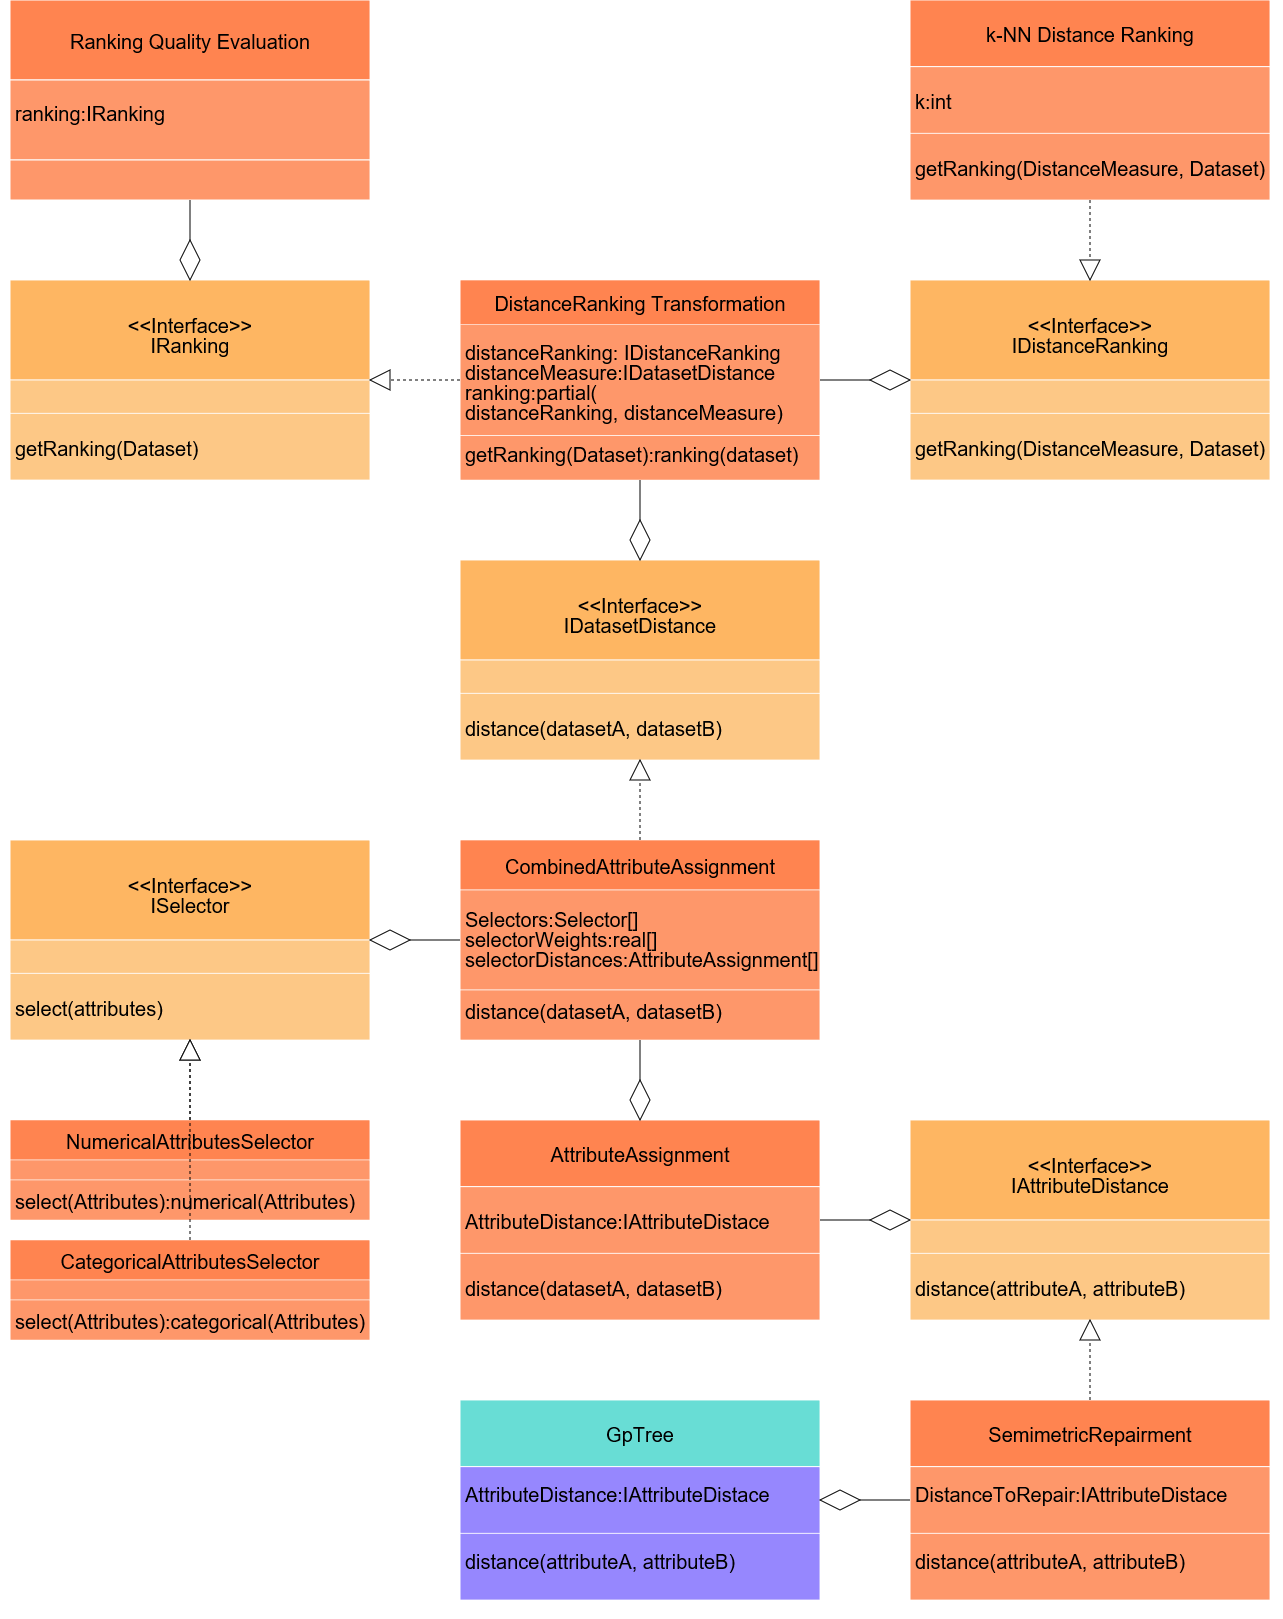
\includegraphics[width=15cm]{Images/BigPictureGp.png}
 	\centering
 	\caption{UML diagram of the workflow for the GP experiments. This time the focus will be on the GP tree, which is going to be evolved using the genetic programming by the fitness from the Ranking Quality Evaluator.}
 	\label{fig:BigPictureGp}	
 \end{figure}
 
 \subsection{Results}
 The results are shown in Table \ref{table:gpResults}. The GP managed to get above the baseline on the validation set in three out of 10 cases. It is not surprising that the statistical comparison of the GP and other algorithms shown in Table \ref{table:gpResultsComparisonWithOthers} resulted in all algorithms except the baseline outperforming the GP.
 
 These poor results could be explained by overfitting, as the training results were decent enough. For example, bloating occurred -- in the first generation the average number of nodes was around one hundred after the initialization. We could observe values above one thousand in the generation 70. This is not a rare behaviour of algorithms with high expression capabilities, as they can very easily learn some noise present in the training data. In the next chapter, we will try to improve generalization abilities of the trees being evolved.
 
 \begin{table} 
 	\caption{Evaluation of the ranking quality of the trees produced by the GP algorithm on the testing dataset.}
 	\label{table:gpResults}
 	\centering 
 	\renewcommand{\arraystretch}{1.3}
 	\begin{tabular}{c c}
 		\hline %inserts horizontal line
 		Run &  GP Result\\
 		\hline 
 			1 & 0.546221	 \\ 
 			2 &	0.542101 \\
 			3 & 0.541881 \\
 			4 & 0.540339 \\
 			5 &	0.538439 \\
 			6 & 0.536444 \\
 			7 &	0.536215 \\
 			8 & 0.532274 \\
 			9 & 0.530289 \\
 			10& 0.512501 \\
 			median & 0.537441 			 	
 	\end{tabular}
 \end{table}
 
 \begin{table}[ht]		
 	\centering
 	\caption{Statistical comparison of GP and previous algorithms and their ranking quality results on the validation set. Y stands for GP significantly worse than algorithm in the corresponding column, N stands for Not able to reject the null hypothesis (algorithms equally performing). }
 	\label{table:gpResultsComparisonWithOthers}	
 	\begin{tabular}{r|cccccccccc}
 		&
 		\rot{Aggregation, $p=1$} &
 		\rot{Aggregation, $p=2$} &
 		\rot{Global, $p=\inf$} &
 		\rot{Global, $p=1$} &
 		\rot{Global, $p=2$} &
 		\rot{Aggregation, $p=\infty$} &
 		\rot{Assignment, $p=2$} &
 		\rot{Assignment, $p=\infty$} &
 		\rot{Assignment, $p=1$} &
 		\rot{Baseline} 		
 		
 		\\ \hline
 		GP        & Y  & Y & Y & Y&Y &Y &Y &Y &Y & N  \\   		
 		\hline
 	\end{tabular} 
 \end{table}
% Experiments
\chapter{Regularization}
\label{chapter:regularization}
In the previous chapter, we relaxed the metric assumptions a little bit, and we proposed a genetic programming algorithm to evolve trees measuring attribute distance that fit into our workflow. 
In the experiments, we observed very poor results of the algorithm ranking model produced by the GP caused by overfitting. 
In this chapter, we will focus on improving the generalization abilities of the GP algorithm. There are many ways how to do that. We will review some of them. The so called \emph{bootstrapping} modifies the initialization phase. Some individuals with already interesting fitness are inserted into populations and their useful blocks may be distributed over the population.
\emph{Regularization} \cite{LearningFromData} is a set of techniques aiming for boosting the generalization abilities of machine learning model. This is done by penalizing complex hypothesis or by encouraging the properties that we think help in generalization. In this chapter, we will introduce two regularization techniques that we believe could help in improving our models -- both of them have been already used in our experiments in \cite{jaCEC2015,jaSSCI2015}. The first approach uses technique called \emph{coevolution} during the evolution of the trees. The second approach -- called \emph{multi-objectivization} -- splits the single objective into multiple objectives in which we can measure some other interesting properties. To do that, we will need a \emph{multi-objective optimization} algorithm. We will present \emph{NSGA-II} algorithm as it is one of the best for two-objective optimization. We will propose new batch of experiments combining genetic programming algorithm from the previous chapter with some of the techniques discussed in this chapter. We will again compare their results with the rest of the algorithms. We also review some of our previous experiments using multi-objectivization for the algorithm ranking problem.

\section{GP Modifications}
In this section, we will review two techniques of modifying the GP algorithm -- bootstrapping and coevolution. Both can be used to improve the generalization abilities of the GP algorithms.

 \subsection{Bootstrapping} 
 The \emph{bootstrap} problem may occur in complex domains. When the population is initialized, all individuals often have very low fitness. This happens especially when the ratio of good to bad solutions is very small. It is then hard for the genetic programming algorithm to estimate good places to evaluate and the run of the algorithm is similar to the random walk algorithm. 
 
 One approach to deal with the bootstrap problem is proposed in \cite{bootstrapIncrementalEvolution}. The problem and/or domain is simplified, so there is a better chance that some good individuals are generated during initialization. After sufficient solutions are found for the simplified problem/domain, we increase the difficulty of the problem but let the population as it is. We expect that the solutions for simplified problems will not have very low fitness for the more difficult problem (as would probably happen with random initialization). The whole process is repeated until the more difficult problem is equal to our original problem. This approach is called the \emph{incremental evolution}.  
 
 The second approach arises from the research about initializing the population \cite{initialpopulationMetricApproach}. If the initial population to the GA is good, then the algorithm has a better possibility of finding a good solution \cite{DiversityAnalysisOfMeasuresAndCorrelationWithFitness}, \cite{ComparisonOfMultiobjectiveEvolutionaryAlgorithm} to seed the GP with that information \cite{GAInitSeedHuntingSnakes}, i.e., the initial population is seeded with some of those possible solutions or partial solutions of the problem. It can be easily combined with some other algorithms. Let other algorithms find some possible or partial solution and pass these solution for the GP initialization.
 
 The bootstrapping can be also used to boost the generalization abilities of the GP. We can insert individuals with good generalization abilities with the expectation that useful blocks of information will be distributes over the population, changed in then novel ways while still maintaining the generalization abilities of the original blocks.

\subsection{Coevolution}
In some cases, it may be beneficial to evolve different part of an individual separately.
For example, the GP algorithm presented in the previous chapter simultaneously evolves two tree - one for measuring the distance between numerical attributes, second for evolving distance between categorical attributes. Instead of thinking about this as individuals consisting of pair of trees, we could think of this as two species - categorical and numerical one. The fitness of an individual would be based on a cooperation of this individual with one or more individuals of the other species. In this case, for one tree for measuring distance between numerical attributes, in each generation, we would choose one or more categorical trees and evaluate ranking quality of this tuple. This has the negative effect that the fitness has to be reset after each generation as the fitness of an individual can change, as the fitness is dependent on the population of other species, which increase the computation time as we cannot pass the fitness of unchanged individuals to the next generation. This does not concern us too much, as this increase is not in the order of magnitudes. The major benefit is that the individual does not have time to overfit, as the stable part is needed for overfitting. Since each generation connects different representations of each species together, only those properties that are generally useful are usually kept in the individuals. More information about coevolution can be found in \cite{WeigandCooperativeCoevolutionaryAlgorithmsAnalysis,PotterJongEvolvingComplexStructuresCoevolution, PotterArchitectureforEvolvingCoadaptedSubcomponents, PotterComputationalModelofCooperativeCoevolution}.

\section{Multi-objectivization}
\label{section:multiobjectivization}
Even if some problem at hand is in fact single-objective (we try to minimize
the error rate of the algorithm), it can be sometimes also expressed as a problem with more
objectives. Such an approach is called \emph{multi-objectivization} and it has
been shown that it can improve the performance of single-objective optimization algorithms,
especially in cases where the optimized function contains plateaus
\cite{BrockhoffAO}. Pil\'at and Neruda \cite{pilat2013multi} used
multi-objectivization for the hyper-parameter tuning of classifiers. They
added two objectives to guide the search -- the root mean squared error and the
kappa statistic -- while they tried to optimize the hyper-parameters for the best
accuracy of the model. In the field of machine learning, multi-objective
optimization can also be used for regularization \cite{multiML}. In such case,
the regularizing term is added as another objective rather than summing it with
the optimized criterion.

Throughout this thesis, we discussed many attribute distance measures. We began with attribute distance measures that were metric, in Chapter \ref{chapter:metricRelaxation} we relaxed this a little bit and discussed semimetrics. We can use the multi-objectivization to add an extra objective to the original one -- resulting ranking quality. The second criterion will be the similarity of a distance measure to a metric. We have two choices for which measure we would like to use. We have an attribute and dataset distance measures. As our training set covers only a limited number of datasets and attributes out of dataset and attribute space, Theorem \ref{theorem:metricPreservationSuportedSpaces} and Observation \ref{theorem:metricNonRestorationSupportedSpaces} will be useful. According to those, the optimization towards a metric on the training datasets does not optimize metric on the attributes in the training dataset, but the opposite is true. In that sense, the optimization towards metric on the attribute space is somewhat stronger. 

As the multi-objective optimization is more complex than single-objective optimization, we will devote some space to a brief introduction. We will formally define a multi-objective optimization problem, discuss Pareto dominance and the first Pareto front. We also introduce NSGA-II algorithm and discuss why it is suitable for our needs.

\subsection{Multi-objective Optimization}
\begin{definition}
	A \emph{multi-objective optimization} problem is defined as a
	tuple \\ $\langle D, O, F, C \rangle$, where $D$ is the design (decision) space, $O \subseteq R^n$ is
	the objective space, $F = \langle  f_1, \dots , f_n \rangle$ with $f_i: D \rightarrow \mathbb{R}$ is the set of $n$ objective functions, and $C = \lbrace c_1, \dots, c_l \rbrace$ is the set of $l$ constraints.
\end{definition}

There are some challenges to overcome compared to single-objective optimization. With the single optimization, the solutions are linearly order according to $f$. This may not apply to multi-objective problems, as it may be the case that $f_1(x)$ is better than $f_1(y)$ but at the same time $f_2(y)$ has better objective value than $f_2(x)$.
This is formalized by the definition of Pareto dominance.
\begin{definition}
	Individual $x$ \emph{Pareto dominates} individual $y$ ($x \prec y$)(equivalently, individual $y$ is Pareto dominated by the individual $x$), if for each objective $f_i:$ $f_i(x) \le f_i(y)$, and there is at least one objective $f_i$ for which $f_i(x) \ne f_i(y)$.
	
	If neither ($x \prec y$) nor ($x \succ y$), we say that $x$ and $y$ are (mutually) \emph{non-dominated}. 
\end{definition}
Pareto dominance is not a total order on $D$, if there is a pair that is mutually non-dominated. This gives a notion to a goal of the multi-objective optimization, as we will be looking for the set that is not dominated by other elements in $D$.
\begin{definition}
	The \emph{solution of multi-objective optimization} problem $\langle D, O, F, C \rangle$ is a Pareto set $P \subset D$, such as for each $x \in D$ and $y \in P$, the individual $y$ is not dominated by the individual $x$. The image of the Pareto set $P$ under the objectives $F$ is a subset of $O$ called the \emph{Pareto front}.
\end{definition}
In practise, finding the enumeration of the solution of the multi-objective optimization problem is often not possible because the solution may be uncountable because it can be uncountable subset of $\mathbb{R}$. If the goal is to enumerate the solution and not to provide function of all elements in the Pareto set, no algorithm can provide a complete solution. This gives a notion of approximation of the solution:
\begin{definition}
	A Pareto set approximation $A \in D$ is a finite set of pints in the decision space such that for each two points $x,y \in A$, $x$ and $y$ are mutually non-dominated.
\end{definition}

\subsection{Multi-objective Evolutionary Algorithms}
There has been a large number of multi-objective evolutionary algorithms proposed in the
past. Examples are the Non-dominated Sorting Genetic Algorithm (NSGA \cite{nsga}), NSGA-II \cite{nsgaII} and Multi-objective Covariance Matrix Adaptation Evolution Strategy (MO-CMA-ES) \cite{IgelCovarianceMatrixAdaptation}. For more complete survey of multi-objective evolutionary algorithms please refer to \cite{BingdongManyObjectiveEvolutionaryAlgorithmsSurvey} and \cite{ZhouMultiobjectiveEASurvey}.

In this thesis, we will use NSGA-II. Although
this algorithm is rather old, it is still among the best optimizers for
two-objective problems \cite{IshibuchiReviewMOEA}. Newer algorithms usually outperforms NSGA-II when the number of objective functions is high. In this case, almost all solutions in the population become non-dominated and the convergence property of the algorithm becomes severely deteriorated. In this thesis, we will have at most two objectives, therefore the NSGA-II algorithm is a suitable choice. 
The main idea of the algorithm is its environmental selection. The evolution prefers individuals who dominate more and who bring more diversity to the population. NSGA-II first sorts individuals to numbered sets called fronts. Individuals from some front dominate all individuals from the fronts with the higher number. Each individual is assigned the number of its front called rank. Compared to its predecessor NSGA where assigning the individuals according to their front took $\mathcal{O}(MN^3)$ time, where $N$ is the population size and $M$ number of objectives, the fast Non-dominated sort outlined in Algorithm \ref{algo:fastNonDominatedSort} reduced the time complexity to $\mathcal{O}(MN^2)$.
The diversity in each front is empowered by so called distance. Individuals in each front with bigger differences in its objectives are preferred. The boundary individuals (with at least one objective being the highest or the lowest in its front) are labelled as most distant. The assignment of the distance to each individuals is outlined in Algorithm \ref{algo:crowdingDistanceAssignment}. 
Given the notion of rank and distance, we can define the partial order $\prec_n$ that the algorithm uses to guide the evolution:
\begin{equation*}
x \prec_y \text{ if } x.rank < y.rank,
\end{equation*}
\begin{equation*}
x \prec_y \text{ if } x.rank = y.rank \text{ and } x.distance > y.distance.
\end{equation*}
That is we prefer solutions with better rank. In the case of a tie, we prefer individuals with better distance.
To ensure elitism (i.e. the fact that the best found solutions are not
lost during the selection), NSGA-II first merges the parent and children
population and the ranks are assigned based on the merged population.
Another important feature of NSGA-II are the operators which are
used. The usual crossover operator is the so called \emph{simulated binary crossover} (SBX) \cite{DebAgravalSimulatedBinaryCrossover}. This operator performs
arithmetic crossover (i.e. it makes a weighted average of two parents),
but the weights are selected in such a way that the change in the
values of the variables is similar to the change of variables when
one-point crossover on binary encoded strings is used. Basically, it
means that the variables of the offspring have higher probability to be
closer to one of the parents than if the weights are selected uniformly.
The mutation operator \cite{DebGoyalCombinedGeneticAdaptiveSearch} – called Polynomial Mutation uses a similar idea. The relative changes in the values of the
variables should be similar to those of a bit-flip mutation on binary
strings.
The generation increment of the NSGA-II is described in Algorithm \ref{algo:nsgaII}. The complexity of each increment is as follows:
\begin{enumerate}
	\item Nondominated sorting is $\mathcal{O}(M(2N)^2)$.
	\item Crowding-Distance assignment is $\mathcal{O}(M2N\log(2N))$.
	\item Sorting on $\prec_n$ is $\mathcal{O}(2N\log(2N))$.
\end{enumerate}
The $N$ stands for the population size and $M$ is the number of objectives.
Total complexity of the generation increment is $\mathcal{O}(MN^2)$.

\IncMargin{1em}
\begin{algorithm}	
	\SetKwInOut{Input}{input}
	\SetKwInOut{Output}{output}
	\tcp{Pseudocode for computing the rank of individuals.}
	\Input{$I\leftarrow$ List of individuals}
	\BlankLine	
	\ForEach{$p$ in $I$}{
		$S_p \leftarrow \emptyset$\;
		$n_p \leftarrow 0$\;
		\ForEach{$q$ in $I$}{
			\If{$p \prec q$}{
				$S_p \leftarrow S_p \bigcup \lbrace q \rbrace$\;
			}
			\ElseIf{$q \prec p$}{
				$n_p \leftarrow n_p+1$\;
			}
		}
		\If{$n_p=0$}{
			$p_{\text{rank}} \leftarrow 0$\;
			$F_1\leftarrow F_1  \bigcup \lbrace p \rbrace$\;
		}
	}
	$i=1$\;
	\While{$F_i \ne \emptyset$}{
		$Q \leftarrow \emptyset$\;
		\ForEach{$p$ in $F_i$}{
			\ForEach{$q$ in $S_p$}{
				$n_q \leftarrow n_q-1$\;
				\If{$n_q = 0$}{
					$q_{\text{rank}} \leftarrow i+1$\;
					$Q \leftarrow Q \bigcup \lbrace q \rbrace$\;
				}
			}
		}		
		$i \leftarrow i+1$\;
		$F_i \leftarrow Q$\;
	}
	\caption{Fast-non-dominated Sort}\label{algo:fastNonDominatedSort}
\end{algorithm}\DecMargin{1em}

\IncMargin{1em}
\begin{algorithm}	
	\SetKwInOut{Input}{input}
	\SetKwInOut{Output}{output}
	\tcp{Pseudocode for computing distance between individuals in the Pareto front. The distance is used by the NSGA-II to maintain diversity in the Pareto front.}
	\Input{$F\leftarrow$ List of objectives}
	\Input{$I\leftarrow$ List of individuals}
	\BlankLine
	size $=$ len$(I)$\;
	\ForEach{$i$ in $I$}{
		$i.\text{distance} \leftarrow 0$\;
	}
	\ForEach{$f \in F$}{
		$I \leftarrow \text{sort}(I,f)$\;
		$I[0].\text{distance} \leftarrow I[\text{size}-1].\text{distance} \leftarrow \infty$\;
		$f_{\min} \leftarrow f(I[0])$\;
		$f_{\max} \leftarrow f(I[\text{size}-1])$\;
		\For{\upshape $k$ in $\lbrace 1,\dots, \text{size}-2 \rbrace$}
		{
			$I[k].\text{distance} \leftarrow I[k].\text{distance}+
			\cfrac{f(I[k-1])+f(I[k+1])}{f_{\max}-f_{\min}}$\;
		}
	}
	\caption{Crowding Distance Assignment}\label{algo:crowdingDistanceAssignment}
\end{algorithm}\DecMargin{1em}
\IncMargin{1em}
\begin{algorithm}
	\SetKwInOut{Input}{input}
	\tcp{Pseudocode for population increment of the NSGA-II algorithm.}
	\Input{$P_t\leftarrow$ Parent population in the time $t$}
	\Input{$Q_t\leftarrow$ Offspring population in the time $t$}
	\BlankLine
	$R_t \leftarrow Q_t \bigcup P_t$\;
	$F \leftarrow \text{fast-non-dominated-sort}(R_t)$\;
	$P_{t+1} \leftarrow \emptyset$\;
	$i \leftarrow 1$\;
	\While{$|P_{t+1}|+|F_i| \le N$}{
		$\text{crowding-distance-assignment}(F_i)$\;
		$P_{t+1} \leftarrow P_{t+1} \bigcup F_i$\;
		$i \leftarrow i+1$ \;
	}
	$\text{sort}(F_i,\prec_n)$\;
	$P_{t+1} \leftarrow P_{t+1} \bigcup F_i[1:(N-|P_{t+1}|)]$\;
	$Q_{t+1} \leftarrow \text{apply-operators}(P_{t+1})$\;
	\caption{NSGA-II}\label{algo:nsgaII}
\end{algorithm}\DecMargin{1em}  
 
 \section{Experiments}
In the new experiments, we will be amending the experiments used in Chapter~\ref{chapter:metricRelaxation}. We will propose experiments using bootstrapping, coevolution and antibloat operators and compare their results with the rest of the algorithms used in this thesis. We will also present the results of our multi-objectivization experiments for the algorithm ranking problem. These were performed over the similar, though not the same, dataset.

 \subsection{Coevolution}
 To implement coevolution, we will amend the GP algorithm presented in Chapter~\ref{chapter:metricRelaxation}. The algorithm evolved both trees as one individual. We will split the population into two, one will correspond to the numerical and second to the categorical population. The functions and terminals for each population will be also split accordingly. In every generation we will generate random bijection between categorical and numerical trees. We will calculate the fitness as if these two trees would be a single individual, and we will still use the fitness from the original GP algorithm. 
 
 We would require about 150 nodes to represent the weighted attribute metric from Chapter \ref{chapter:metricExperiments}. It is difficult for the GP to find similar distance measures as the search space is very big. Therefore, we decided to try bootstrapping so the GP can use the useful components of the metric evolved in the previous experiments. As in the GP experiments, we do not evolve weights. Therefore, we decided to use individuals who did not discriminate between categorical and numerical attributes and whose selector weights were around the same value. We also decided not to use the best individual as we wanted to allow GP algorithm to fine tune the distance itself. It could be hard otherwise to beat the given distance thus creating the same problem again that we are addressing with the bootstrapping.
 
 We have chosen the individual with the numerical weight equal to 2.508826 and categorical to 2.250011. With the weights included, the training fitness was equal to 0.554701 on the training set and to 0.54561 on the testing set respectively.
 As the GP did not incorporated the weights, the fitness slightly changed to 0.553206 on the training set and to 0.544519 on the testing set respectively.
 
 We have not changed any other parameters. 
 
 \subsection{Antibloat}
 In the antibloat experiments we have reused the framework from Chapter \ref{chapter:metricRelaxation}. We have only amended the tournament selection. If the size of the individual exceeds the limit, we decrease the fitness of the individual. This decrease is only for the selection purposes, we have not amended this for the sake of elitism and ranking quality reporting. Let us suppose that we have some individual with fitness $f \in \langle 0,1 \rangle.$ We rescaled the fitness by every of the following, once per each penalty: 
 \begin{enumerate}
 	\item One percent down per each 10 nodes above 200 in the categorical tree.
 	\item One percent down per each 10 nodes above 200 in the numerical tree.
  	\item One percent down per each 5 points above 20 measured in the maximum width of the levels in the categorical tree.
 	\item One percent down per each 5 points above 20 measured in the maximum width of the levels in the numerical tree.
  	\item One percent down per each 5 points above 20 measured in the maximum depth of the levels in the categorical tree.
  	\item One percent down per each 5 points above 20 measured in the maximum depth of the numerical tree. 	
 \end{enumerate}  
We set a cap to every such rescaling to 0.9, as we did not want a single penalty to completely negate the fitness of particular individual.
Furthermore, we did not allow the fitness to become less than zero. 
 
 \subsection{Results}
 The results of individual runs of the GP algorithm with antibloat operator and coevolution with bootstrapping can be found in Table \ref{table:gpCoevolutionResults}. Statistical comparison with the results of the previous algorithms can be found in Table \ref{table:gpCoevolutionResultsComparisonWithOthers}. The algorithm with bootstrapping and coevolution managed to beat the baseline and all the pure assignment based algorithms. It also managed to match the level of the first combination of the global metafeatures and assignments. In some runs the overfitting was still present -- although the algorithm managed to improve the fitness on the training set, in some cases it did not improve the results on the validation set. That significantly decreased its score in the overall results. However, one run managed to outperform every other run using the global attributes only and produced one of the best results using solely the assignments. This suggest that attribute assignment has a very good potential to be improved with further empowering the generalization abilities of GP algorithm.
 The runs with the antibloat operator reduced bloating, however we did not observe a big difference in the resulting ranking quality. This suggests that the bloating is not the only factor reducing the generalization abilities.
 
 \begin{table} 
 	\caption{Evaluation of the ranking quality of the trees produced by the GP algorithm using antibloat operator and bootstrapping with coevolution on the testing dataset.}
 	\label{table:gpCoevolutionResults}
 	\centering 
 	\renewcommand{\arraystretch}{1.3}
 	\begin{tabular}{c c l}
 		\hline %inserts horizontal line
 		Run &  Coevolution+Bootstrap & Antibloat\\
 		\hline 
 		1 & 0.559953 & 0.553059 \\ 
 		2 &	0.553473 & 0.54562 \\
 		3 & 0.552748 & 0.543022 \\
 		4 & 0.551044 & 0.541717 \\
 		5 &	0.550729 & 0.5394 \\
 		6 & 0.548995 & 0.539193 \\
 		7 &	0.548331 & 0.533419 \\
 		8 & 0.548253 & 0.532851 \\
 		9 & 0.544634 & 	0.53082 \\
 		10 & 0.544221 & 0.528787 \\
 		median & 0.549862 & 0.539297
 				 	
 	\end{tabular}
 \end{table}
 
 \begin{table}[ht]		
 	\centering
 	\caption{Statistical comparison of GP using antibloat operator and coevolution with bootstrapping and previous algorithms and their ranking quality results on the validation set. W stands for GP statistically worse than the algorithm in the corresponding column, I stands for inconclusive and B stands for statistically better. }
 	\label{table:gpCoevolutionResultsComparisonWithOthers}	
 	\begin{tabular}{r|cccccccccccc}
 		&
 		\rot{Coevolution+Bootstrap} &
 		\rot{Aggregation, $p=1$} &
 		\rot{Aggregation, $p=2$} &
 		\rot{Global, $p=\inf$} &
 		\rot{Global, $p=1$} &
 		\rot{Global, $p=2$} &
 		\rot{Aggregation, $p=\infty$} &
 		\rot{Assignment, $p=2$} &
 		\rot{Assignment, $p=\infty$} &
 		\rot{Assignment, $p=1$} &
 		\rot{GP} &
 		\rot{Baseline} 		
 		
 		\\ \hline
 		Coev+Boot & &  W & W & W & W& W &I &B &B & B & B & B  \\   
 		Antibloat & W &  W & W & W & W& W & W & W & I & I & I & I  \\   		
 		\hline
 	\end{tabular} 
 \end{table}
 
 \subsection{Multi-objectivization}
 We have experimented with the multi-objectivization for the algorithm ranking in \cite{jaSSCI2015}. Herein, we have used similar OpenML dump. The difference was in fewer filters applied, as we did not compare with propositional approaches and therefore we did not include the requirements that all datasets have all global metadata available.
 
 The whole workflow was derived from the one used in Chapter \ref{chapter:metricRelaxation}, although we did not explicitly repair the distance function to a semimetric.
 
 As discussed in Section \ref{section:multiobjectivization}, it is better to include metric similarity of the attribute distance instead of dataset distance.
 For that reason we have used resemblance of attribute distance measure $\delta$ to a metric as a second criterion. To be precise, for each selector we measured $$E_{selector}=\frac{e_1 + e_2 + e_3 + e_4}{4},$$
 where $e_i$ is the ratio of instances (tuples of triples) where metric axiom $i$ did not hold. We then based the second criterion on the aggregation of $E$ over all selectors:
  $$f_2 =1 - \frac{\sum_{s \in Selectors}{E_s}}{|Selectors|}.$$
 If we repaired the distance function to a semimetric, as we have already mentioned, it would be enough to measure just the amount of cases where triangle inequality held. 
 
 As a multi-objective algorithm the NSGA-II was chosen. The size of the population was set to 200. The tournament approach was selected as the selection mechanism. A better individual was chosen according to rank and crowding distance. The probability of better individual winning the tournament was set to 0.7. Also, the NSGA-II uses elitism, so the best individual were guaranteed to be copied to the next generation. Tree mutation and crossover were used as genetic operators. The probabilities of mutation and crossover were set to 0.2 and 0.7 respectively. The termination criterion was set to 80 generations. This was mainly we noticed that the bloating usually appeared around this generation.
 
 We have performed seven runs and we obtained significantly better results compared to the baseline algorithm. Furthemore, we have observed the high correlation of the metric similarity and prediction accuracy. This supports the hypothesis that the metric properties are important for the generalization abilities of the induced dataset similarity measure. This was the most obvious during the second run, whose results are depicted in Figures \ref{fig:NSGABestTraining} (training) and \ref{fig:NSGABestValidation} (testing). The Spearman’s rank correlation coefficient between the first and second criterion of the second run on the testing set was 0.734. This means that in the testing set the individuals more similar to a metric had better results for the prediction of the algorithm ranking.
 
\begin{figure}	
	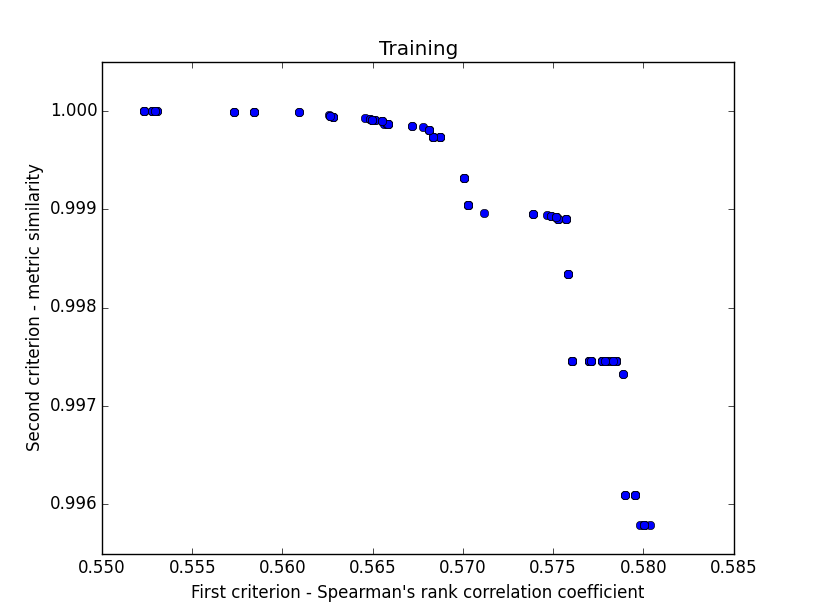
\includegraphics[width=\columnwidth]{Images/nsgaTraining.PNG}
	\centering
	\caption{Results of the first Pareto front of the second run on the training set.}	
	\label{fig:NSGABestTraining}
\end{figure}

\begin{figure}	
	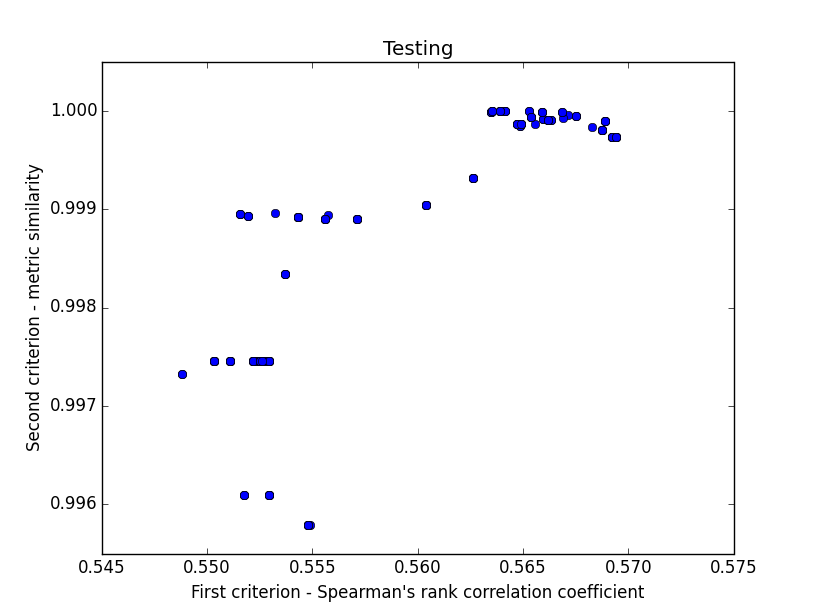
\includegraphics[width=\columnwidth]{Images/nsgaValidation.PNG}
	\centering
	\caption{Results of the first Pareto front of the second run on the testing set. Note the high correlation between both criteria - the higher values of the accuracy criterion are associated with higher values of the metric similarity criterion.}	
	\label{fig:NSGABestValidation}
\end{figure}
% Regularization + Experiments
%\include{chap8}



%TODO: single objective to solve multi objective
% Distance based metalearning - see Hutters paper
% Reference na priklady dalsich genetickych operatoru/modification
% Bootstrapping - simple metrics to GP
% Master thesis alignment is a metric
% Question - muze byt v alignmentu jina funkce nez +?
% Experiment databases - vanschoren
% Diskuze - IRanking interface v quality, aby se nam vypocty neopakovali
%Hyperparameter optimization
%vanschoren expdb

% Ukázka použití některých konstrukcí LateXu (odkomentujte, chcete-li)
% %%% Ukázka použití některých konstrukcí LaTeXu

\subsection{Ukázka \LaTeX{}u}
\label{ssec:ukazka}

This short subsection serves as an~example of basic \LaTeX{} constructs,
which can be useful for writing a~thesis.

Let us start with lists:

\begin{itemize}
\item The logo of Matfyz is displayed in figure~\ref{fig:mff}.
\item This is subsection~\ref{ssec:ukazka}.
\item Citing literature~\cite{lamport94}.
\end{itemize}

Different kinds of dashes:
red-black (short),
pages 16--22 (middle),
$45-44$ (minus),
and this is --- as you could have expected --- a~sentence-level dash,
which is the longest.
(Note that we have follwed \verb|a| by a~tilde instead of a~space
to avoid line breaks at that place.)

\newtheorem{theorem}{Theorem}
\newtheorem*{define}{Definition}	% Definice nečíslujeme, proto "*"

\begin{define}
A~{\sl Tree} is a connected graph with no cycles.
\end{define}

\begin{theorem}
This theorem is false.
\end{theorem}

\begin{proof}
False theorems do not have proofs.
\end{proof}

\begin{figure}
	\centering
	\includegraphics[width=30mm]{../img/logo.eps}
	\caption{Logo of MFF UK}
	\label{fig:mff}
\end{figure}

\chapter{Conclusion}
\label{chapter:conclusion}

In this thesis, we have studied the non-propositional approach for comparing two datasets. We have focused on algorithm ranking problem in metalearning. However, our approach is not limited solely to this area and can be easily reused even in other fields. Specifically, the distance measures defined on some set $\mathbb{X}$ can be transformed by attribute assignment algorithms
to a distance measure on the power set $2^\mathbb{X}$ of $\mathbb{X}.$

The main contribution lies in the design of multiple algorithms for measuring the distance between two datasets that can handle non-propositional metadata and their unique theoretical properties. The difference between them is in the computational complexity, expression power and guarantees on the resulting dataset distance measure.

When proposing our algorithms, we built our work on the related approaches. The literature suggested several methods to handle the non-propositionality, either directly in the metalearning fields or in some other areas of computational intelligence. However, we have identified several areas that could improve the reviewed literature. For instance, the current approaches are either losing important information, lack metric properties or assume that the order is important (although we can reshuffle attributes in datasets without changing the information). This drove our motivation to propose new methods in the first place. Furthermore, authors of \cite{RepresentationalIssuesInMetalearning} recognized the problem of building the distance over non-propositional datasets as non-trivial.

The main idea behind our algorithms rests upon the idea of attribute assignment. To measure distance between two datasets, we first propose an attribute distance measure. We first amend the datasets so their cardinalities match, by inserting artificial attributes into the dataset with less attributes. Then we find bijection of attributes from the first dataset to another so the sum of the distances defined by the bijection and the attribute is minimized. This sum of distances is also the desired distance between datasets.

We have proven that under certain conditions, the resulting distance between datasets is a metric. The main condition for this is that the underlying attribute distance measure itself is a metric. Other conditions include several restrictions on extending the attribute space by a $\dummy$ attribute. We have also proven that the above is valid also in the other directions.
However, the first direction is somewhat stronger if we have only training data and is optimizing towards a metric on either dataset or attribute subspace defined by training data.
Some other ideas were considered, for instance the normalization of the sum of attribute distances by the number of attributes. However, we have proven that this can break the triangle inequality axiom.

We have designed our algorithm to be extensible. It is possible to use the metadata specific for some attribute types, for instance for categorical and numerical metadata. This is achieved by splitting the distance into two, one for each metadata type. We have verified that this does not affect the metric properties of the algorithms. It is also possible to combine multiple metric distance into one. This allows our assignment approach to be combined with propositional approaches. As both approaches return useful information, we argued that by combining them, even more accurate sense of distances between datasets should be obtained.

We have designed generic workflow for measuring quality of ranking. As we made sure that all our algorithms conform to specified interfaces, it is possible to replace different parts of the workflow. This allowed us to compare different algorithms and their combinations proposed in the thesis in a unified way. We have also proven that it is possible to optimize distance based measures without changing their properties. This enabled us to employ optimization methods to boost the performance of our algorithms. We have employed genetic algorithms and genetic programming for this purpose. 

Results of genetic algorithm experiments suggest that attribute alignment algorithms can be successfully used for algorithm ranking. Every parameter settings we optimized produced statistically better results than the baseline algorithm with a single exception. The aggregation of global and attribute approach produced the best results.
With genetic programming, we traded triangle inequality for higher expression power. It was so powerful that it could overfit the training data very easily. To counter this, we have employed several approaches to improve generalization abilities. With this we managed to further improve the results of the assignment algorithms on our data. Especially coevolution combined with bootstrapping of the population managed to obtain promising results. We also reviewed one of our previous work where we used multi-objectivization to boost the generalization abilities of models being evolved. We introduced metric resemblance as a second criterion. Results suggested that there is a high correlation between the second criterion and generalization abilities of the models.

We have also demonstrated visualization of non-propositional dataset representation using the kernelized PCA. We investigated the visualization in more depth, and the results seems to be plausible as the visualisation rendered similar datasets in the same cluster.

\section{Future Work}
The work presented in this thesis can be extended in several directions. We wanted to focus on the attribute based distance. As the whole workflow of all the pieces plugged together became quite complicated, we did not want to add extra parts that would distract from the main idea by increasing the complexity of the workflow. It would be possible however to use ensemble based learning on top of our models to get the combined accuracy of our models. 

As we are using distance based algorithms, it could be beneficial to try better methods, such as weighted $k$-NN, that would make use of the distances of the nearest neighbours. It would also help to have more data. As we are dealing with high dimensional dataset space, hundreds of datasets is still very small amount to reasonably cover the space. 

Our algorithms need lots of parameters. As our resources are limited and the training of models took significant amount of time, we could not dedicate much space to tuning of the parameters, and parameters we used were based on the previous experiments or short preliminary experiments. We would like to tune the parameter of $k$ of the $k$-NN, different parameters and genetic operators of genetic algorithms used, with different strategies for adding the dummy attribute (either constant or different attribute when selected from attribute space). Even in this thesis, we have observed that parameters can significantly improve the overall results of experiments.

We would also like to enhance Genetic Programming algorithm with types. Typed genetic programming \cite{typedGp,tomCec14} can help reduce the space that is searched and allows for more elaborate constructs and operators.

A room for improvement can be also seen in the metafeatures we are extracting from the attributes. Currently, only simple, statistical and theoretical metafeatures are extracted. It could be interesting whether we can extract some sort of landmarks on the attribute level. For example, we can try to predict target values using only a single attribute and use the results as a new metafeatures. It could also help to find metafeatures that are really useful for the generalization. It may well be the case that some metafeatures are just used to overfit the data and instead of contributing to the generalization abilities of the models, they are just downgrading the validation results.

We also see an opportunity in expanding the theoretical work. After the alignment, we use the sum of individual attribute distances given by the assignments to get the metric on datasets provided that certain conditions hold. It could be interesting to see whether some other aggregations can be used without sacrificing the nice property of metric preservations. It could be also beneficial to define sort of normalization of the resulting dataset distance that does not violate metric axioms.

%%% Seznam použité literatury
%\include{bibliography}
\bibliographystyle{plain}
\bibliography{../bibli}

\cleardoublepage
% \phantomsection
\addcontentsline{toc}{chapter}{\listfigurename}
\listoffigures

\cleardoublepage
% \phantomsection
\addcontentsline{toc}{chapter}{List of Algorithms}
\listofalgorithms


\cleardoublepage
% \phantomsection
\addcontentsline{toc}{chapter}{\listtablename}
\listoftables

%Term definitions
\gloss[nocite]{*}

%\setglosslabel{#2}
%This will remove the category
\renewcommand{\glossheading}[1]{% 
	\stopglosslist % -- Don’t forget that! 
}
%	\renewenvironment{glosslist} {\begin{description}} {\end{description}}


\def\glossname{Acronyms}
\printgloss{../glossary}

%%% Přílohy k disertační práci, existují-li (různé dodatky jako výpisy programů,
%%% diagramy apod.). Každá příloha musí být alespoň jednou odkazována z vlastního
%%% textu práce. Přílohy se číslují.
\chapwithtoc{Attachments}
All auxiliary materials including OpenML data dump and the text of the thesis are available at https://github.com/jaksmid/dissertation. 

\openright
\end{document}
